We perform the analysis on a dataset corresponding to \intlumi\ integrated luminosity. 
We document the results obtained after preselections
designed to control the level of agreement between the various background predictions
and the data in Sections \ref{sec:results_zzpresel} and \ref{sec:results_topww}.
The results of the mass-dependent $\hzz$ selections using cut-based 
(see Section~\ref{sec:anal_cutbased}) and shape based (see Section~\ref{sec:anal_mt}) approaches
are then reported in Sections \ref{sec:results_cut} and \ref{sec:results_mtshape} respectively.

\subsection{Results in the Z+Jets control region}
\label{sec:results_zzpresel}

We compare the data with simulation in looser selections than the signal region 
to verfity the agreement in the key kinematic observables that we select on. 

Figure~\ref{fig:npv} shows the number of primary vertices in $ee$ and $\mu\mu$ final states 
after the $\ZZ$ preselections, comparing data to the simulation which was reweighted in the 
number of pile up events to match the values in data. This is a validation of the reweighting procedure. 
Figures~\ref{fig:zmass_zzpresel_mm}-\ref{fig:zmass_zzpresel_ee} show the dilepton mass distributions 
after applying all $\ZZ$ preselections except for the dilepton mass cuts, comparing data 
with simulation for the $\mu\mu$ amd $ee$ final states respectively in different jet 
bin final states. We observe in general a good agreement, except for a slight shift in the 
$\mu\mu$ final states. Figures~\ref{fig:zpt_zzpresel_mm} and~\ref{fig:zpt_zzpresel_ee} 
show the dilepton $p_T$ spectrum after the $\ZZ$ preselections for $\mu\mu$ and $ee$ final states. 
This provides an initial validation of the $\dyll$ background estimation. 

Table~\ref{tab:zzselection_all_4fb} shows the number of events observed in
data, comparing to the expected background contributions after the \zz\ preselections. 
The background estimation was discussed at Section~\ref{sec:backgrounds}. 
We validate the observables that are used in the higgs signal extraction at the 
$\ZZ$ preselection level. 
Figures~\ref{fig:met_zzpresel_mm}-\ref{fig:dphijetmet_zzpresel_ee} show 
the data to simulation comparions of the $\met$, $m_T$ and $\Delta\phi(jet,met)$ distributions. 
Good agreement between data and simulation is observed. 

%%%%%%%%%%%%%%%%%%
\begin{table}[!ht]
\begin{center}
\begin{tabular}{c|c|c|c}
\hline
Process    & $\mu\mu$    & ee     & TOTAL\\ \hline 
%\multicolumn{4}{c} {0-Jet Bin} \\
\zz\ 	& 37.80 $\pm$ 0.20	& 27.05 $\pm$ 0.17	& 64.85 $\pm$ 0.26 \\
$gg\to ZZ$& 3.34 $\pm$ 0.02	& 2.39 $\pm$ 0.02	& 5.73 $\pm$ 0.02 \\ 
$\wz$	& 28.35 $\pm$ 0.31	& 20.52 $\pm$ 0.26	& 48.87 $\pm$ 0.41 \\
Zjets	& 122.73 $\pm$ 5.55	& 85.07 $\pm$ 3.59	& 207.80 $\pm$ 6.61 \\
WW/Top	& 66.51 $\pm$ 6.08	& 53.37 $\pm$ 4.88	& 119.88 $\pm$ 7.80 \\ 
\hline
Total Background	& 258.72 $\pm$ 8.24	& 188.40 $\pm$ 6.07	& 447.13 $\pm$ 10.23 \\
\hline
Data	& 228	& 150 	& 378 \\ 
\hline \hline
\end{tabular}
\caption{Expected number of signal and background events corresponding to an 
integrated luminosity of \intlumi after applying the \zz preselections. 
Only statistical uncertaities are reported. The $\Wjets$ background is neglible thus omitted in the table.
%The background predictions do not have the data-to-simulation scale factors applied. 
}
\label{tab:zzselection_all_4fb}
\end{center}
\end{table}
%%%%%%%%%%%%%%%%%%

%%%%%%%%
\begin{figure}[!hbtp]
\begin{center}
\subfigure[Inclusive]{\label{subfig:npv_mm}
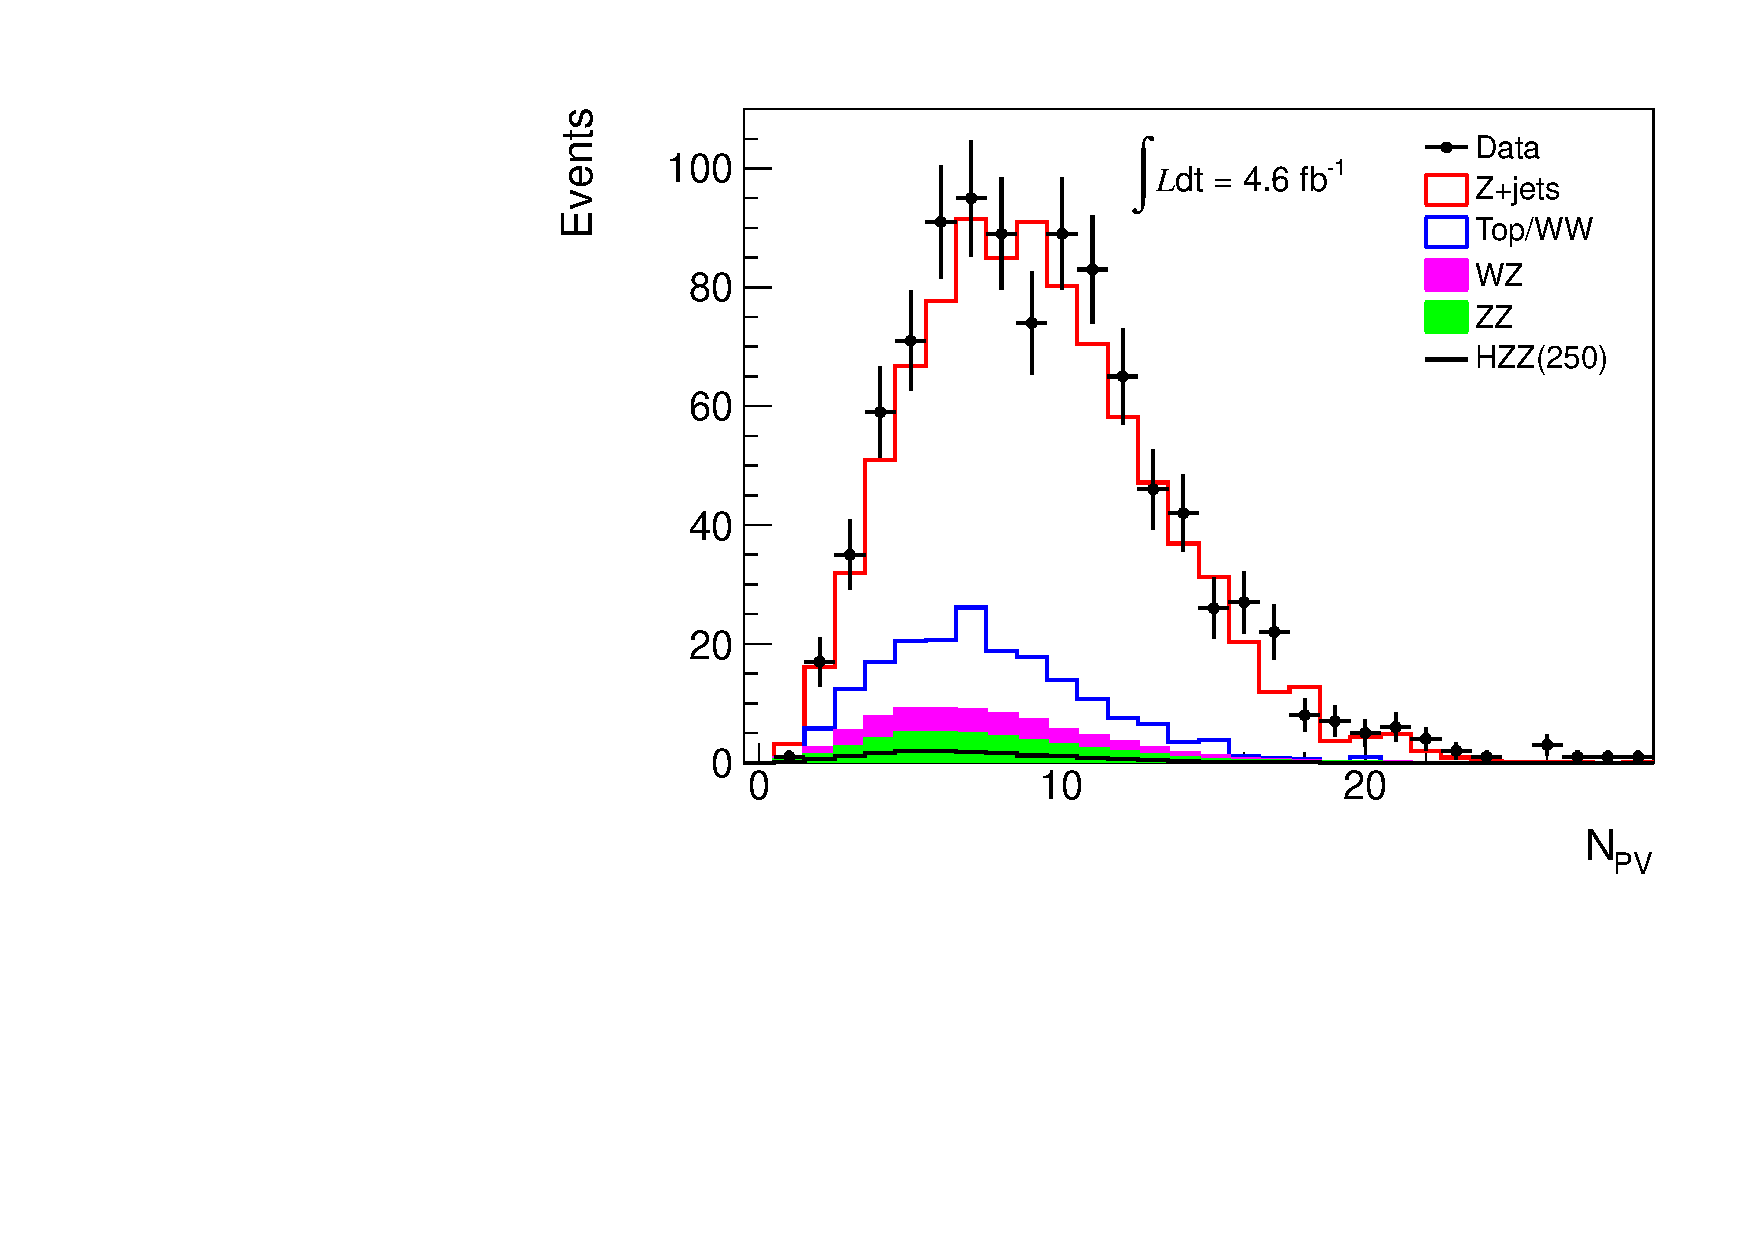
\includegraphics[width=.4\textwidth]{figures/presel_mH250_ee_npv.pdf}}
\subfigure[1-Jet]{\label{subfig:npv_ee}
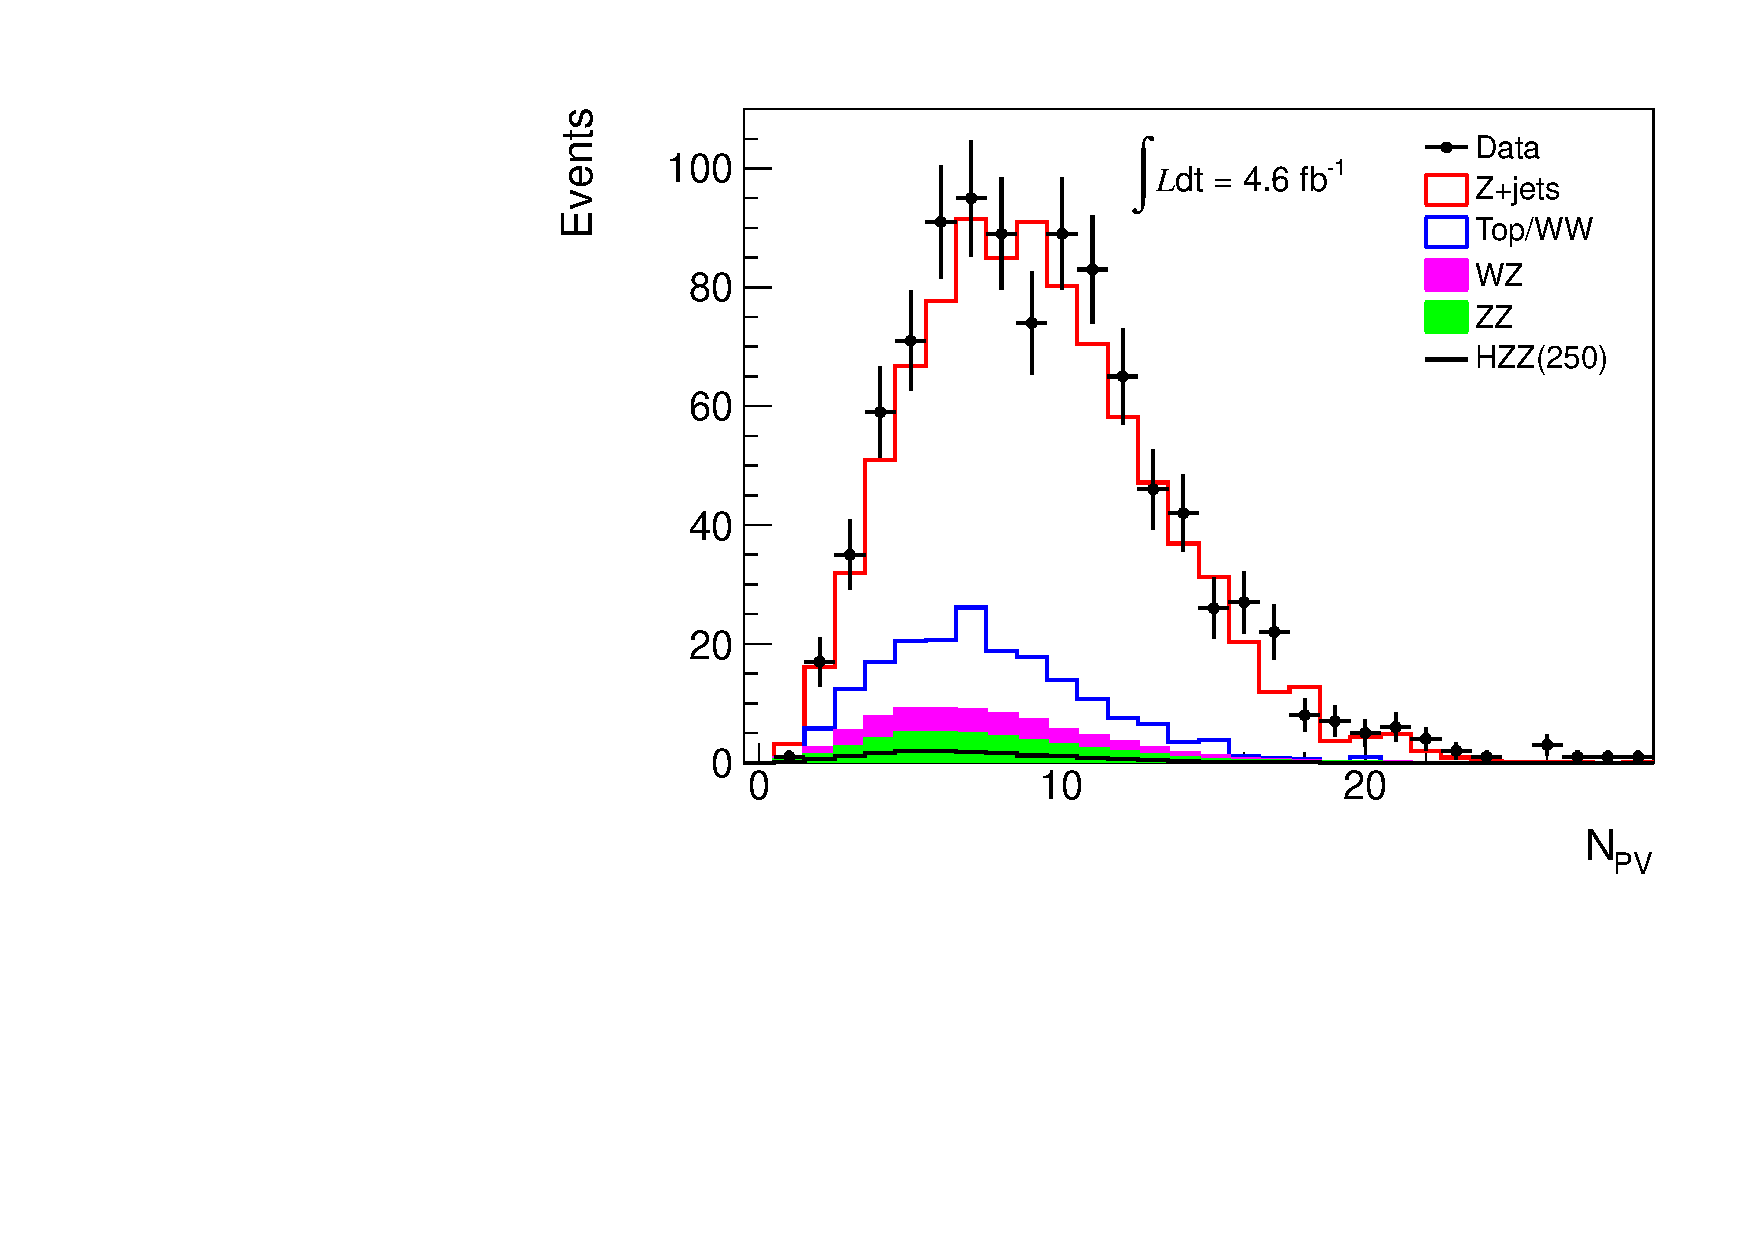
\includegraphics[width=.4\textwidth]{figures/presel_mH250_ee_npv.pdf}}
\caption{Distribution for the number of reconstructed primary vertices after the $\ZZ$ preselection observed in data corresponding 
to $2.1$~\ifb data in the muon~\subref{subfig:npv_mm} and electron~\subref{subfig:npv_ee} channels, compared to the expected from simulation for signal 
and background. The MC backgrounds are scaled as appropriate and the photon+jets estimate of the Z+jets background is added to the stack.}
\label{fig:npv}
\end{center}
\end{figure}
%%%%%%%%

%%%%%%%%
\begin{figure}[!hbtp]
\begin{center}
\subfigure[Inclusive]{\label{subfig:zmass_mm_incl}
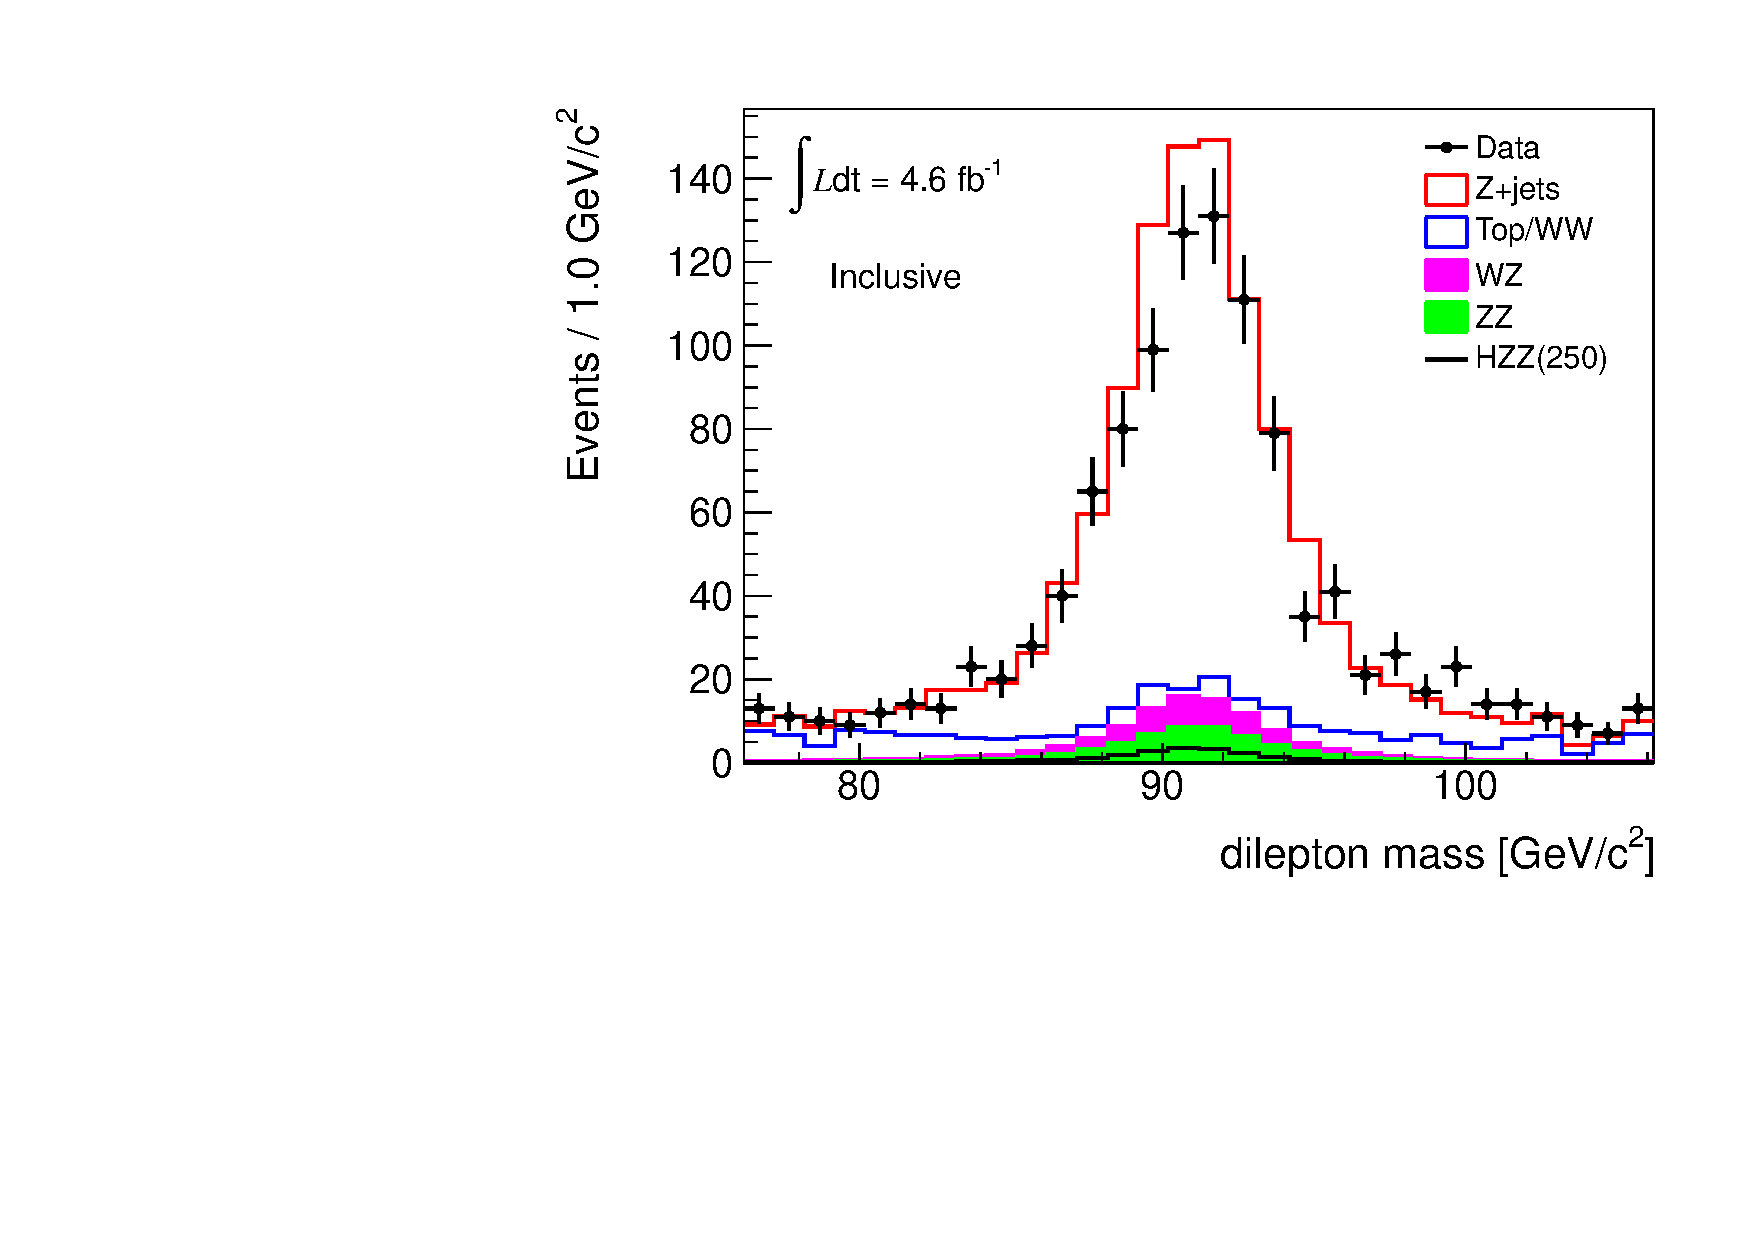
\includegraphics[width=.4\textwidth]{figures/presel_mH250_mm_mass_incl.pdf}}
\subfigure[0-Jet]{\label{subfig:zmass_mm_0j}
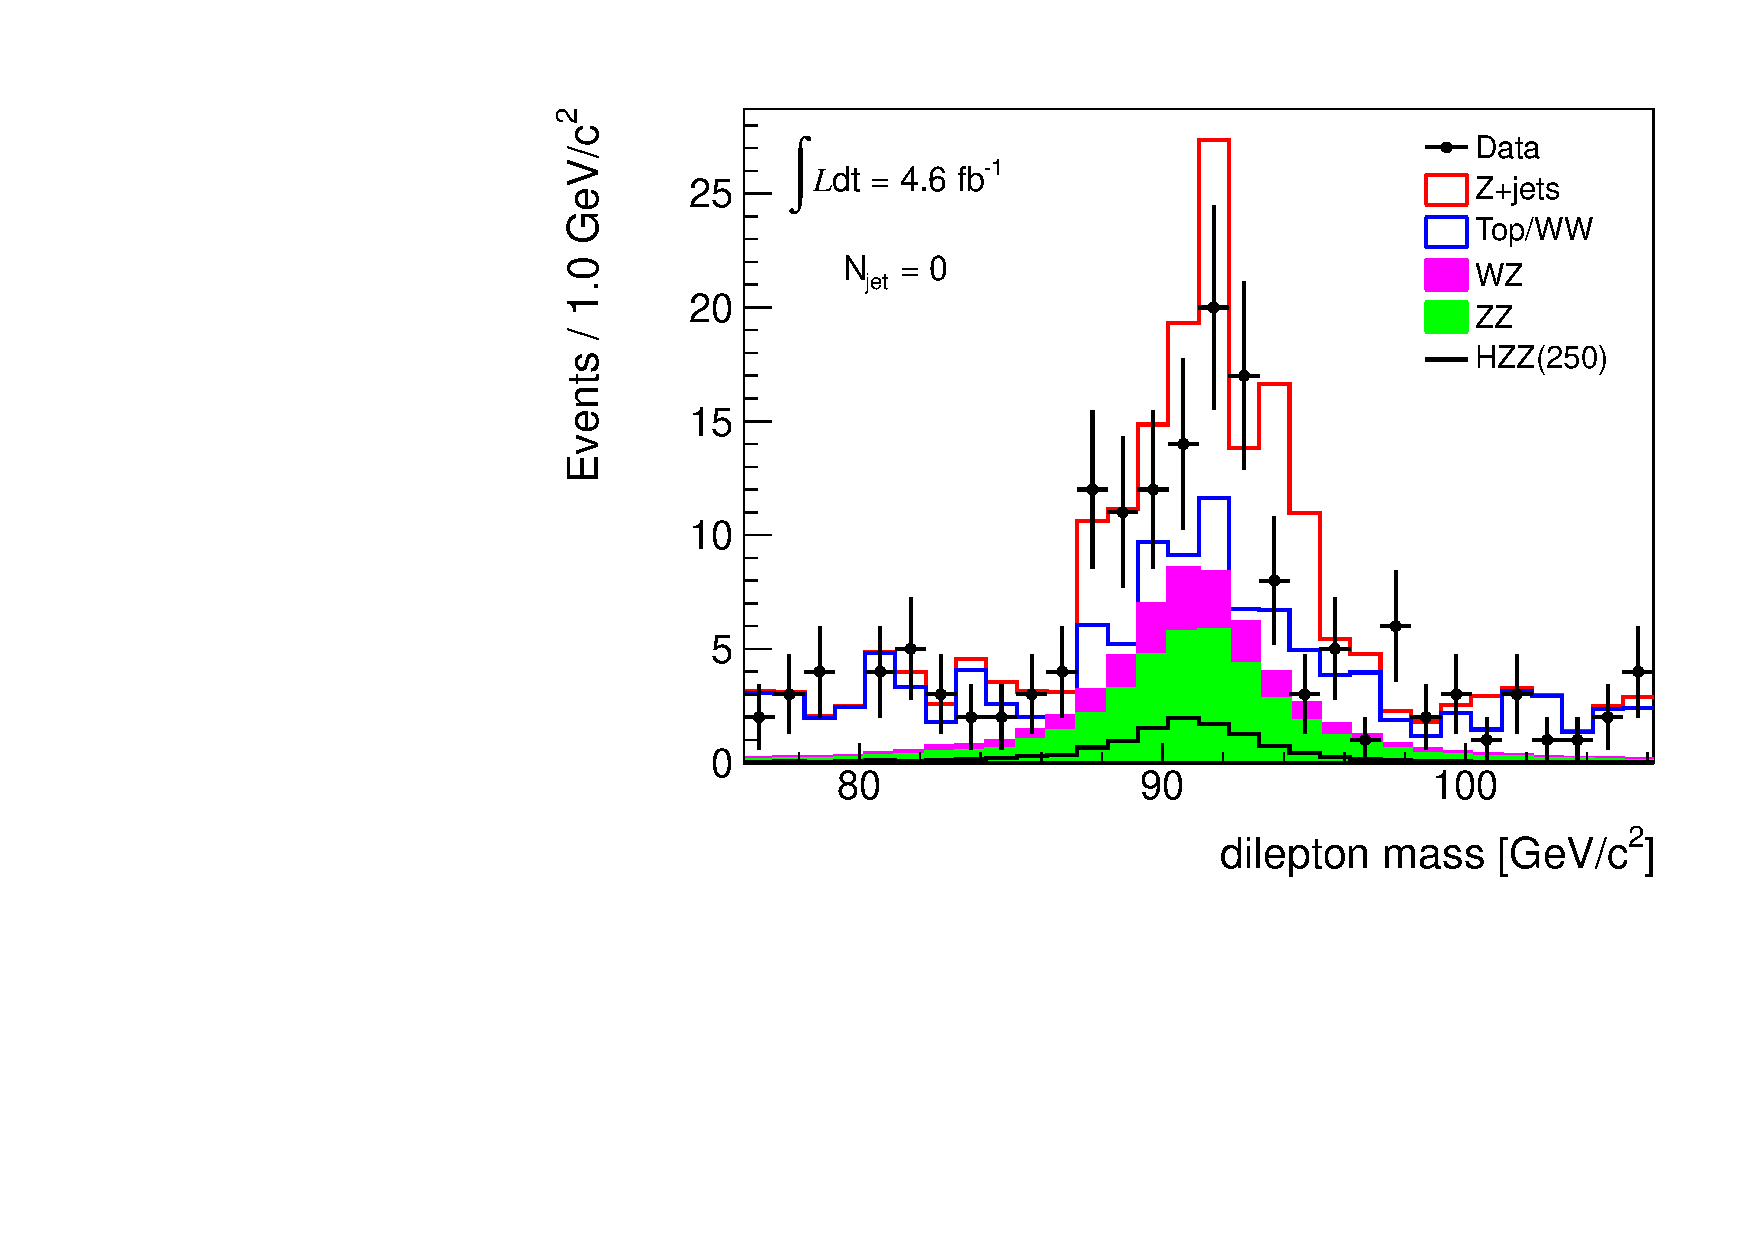
\includegraphics[width=.4\textwidth]{figures/presel_mH250_mm_mass_0j.pdf}} \\
\subfigure[1-Jet]{\label{subfig:zmass_mm_1j}
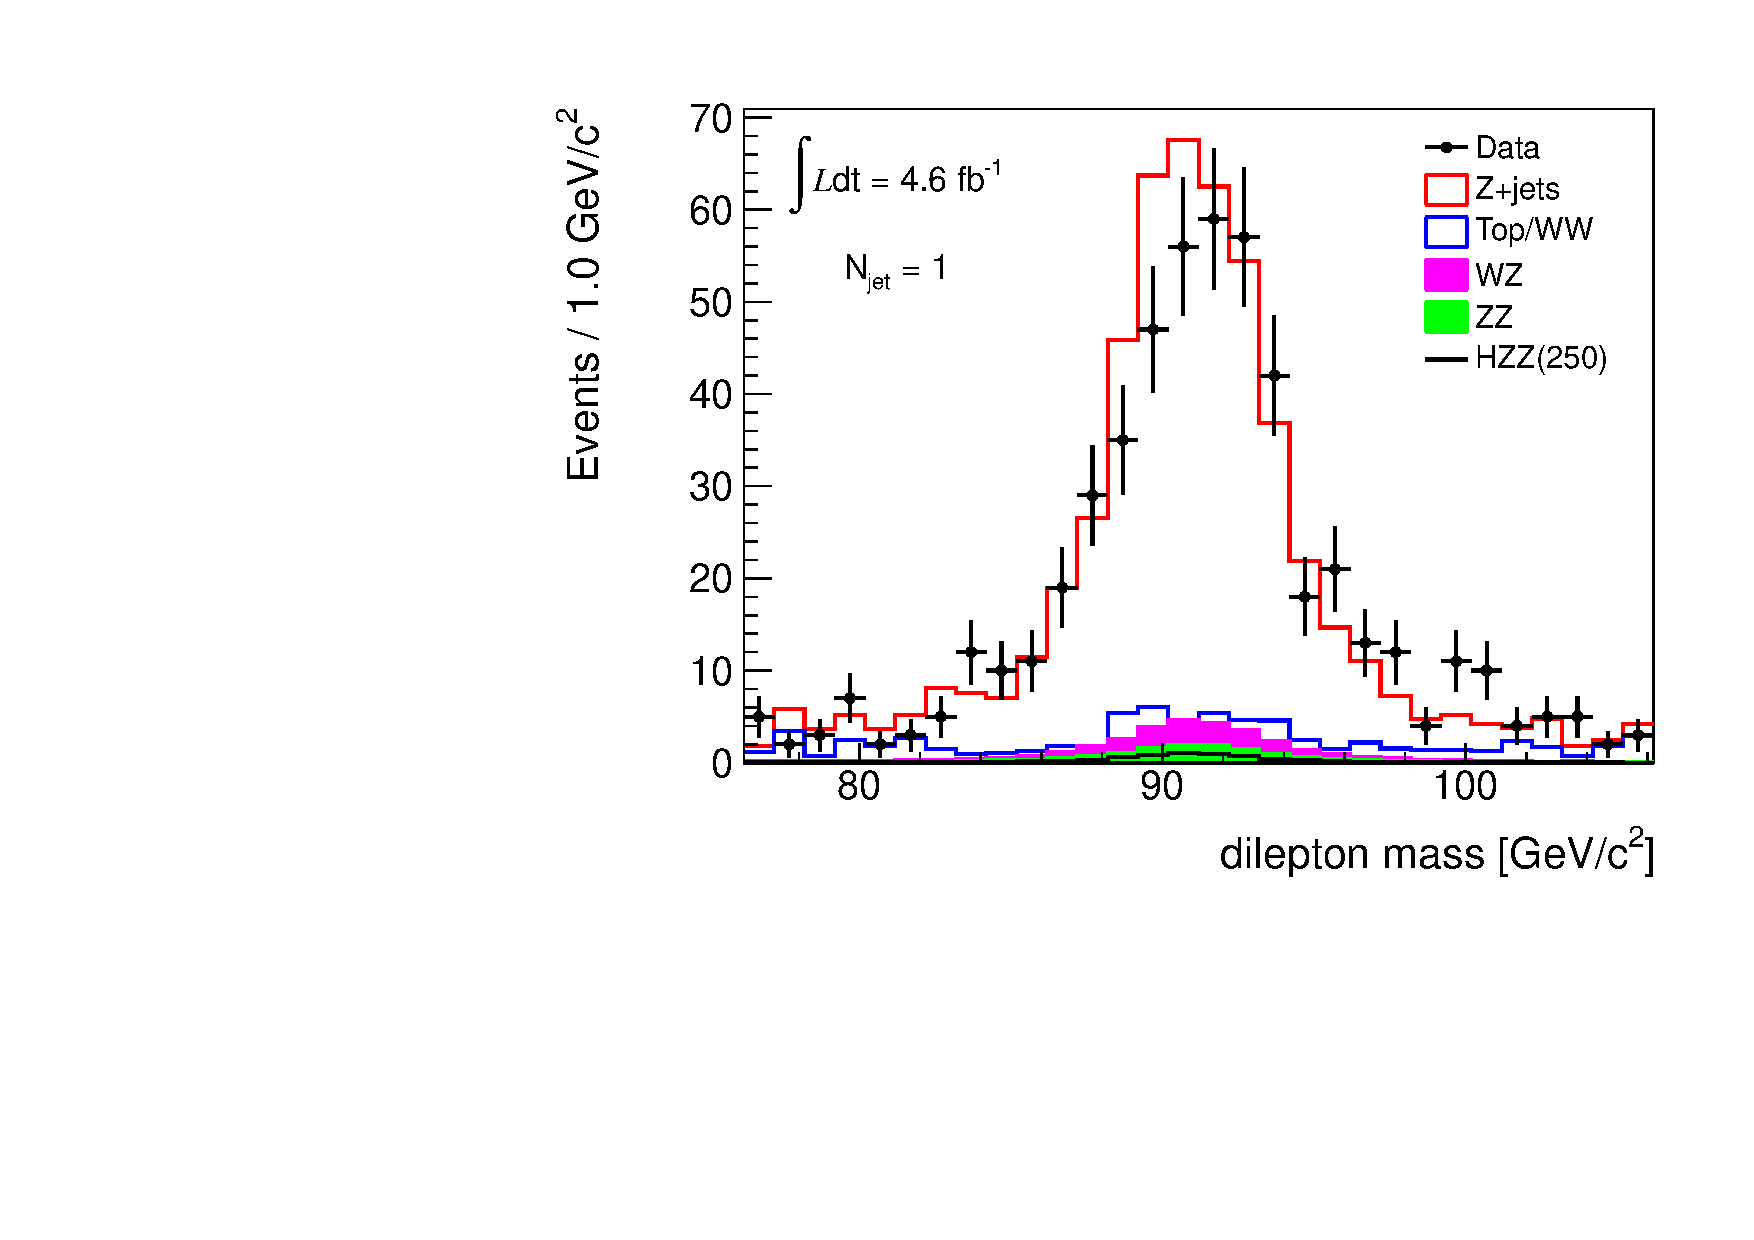
\includegraphics[width=.4\textwidth]{figures/presel_mH250_mm_mass_1j.pdf}}
\subfigure[$\geq$2 Jets]{\label{subfig:zmass_mm_2j}
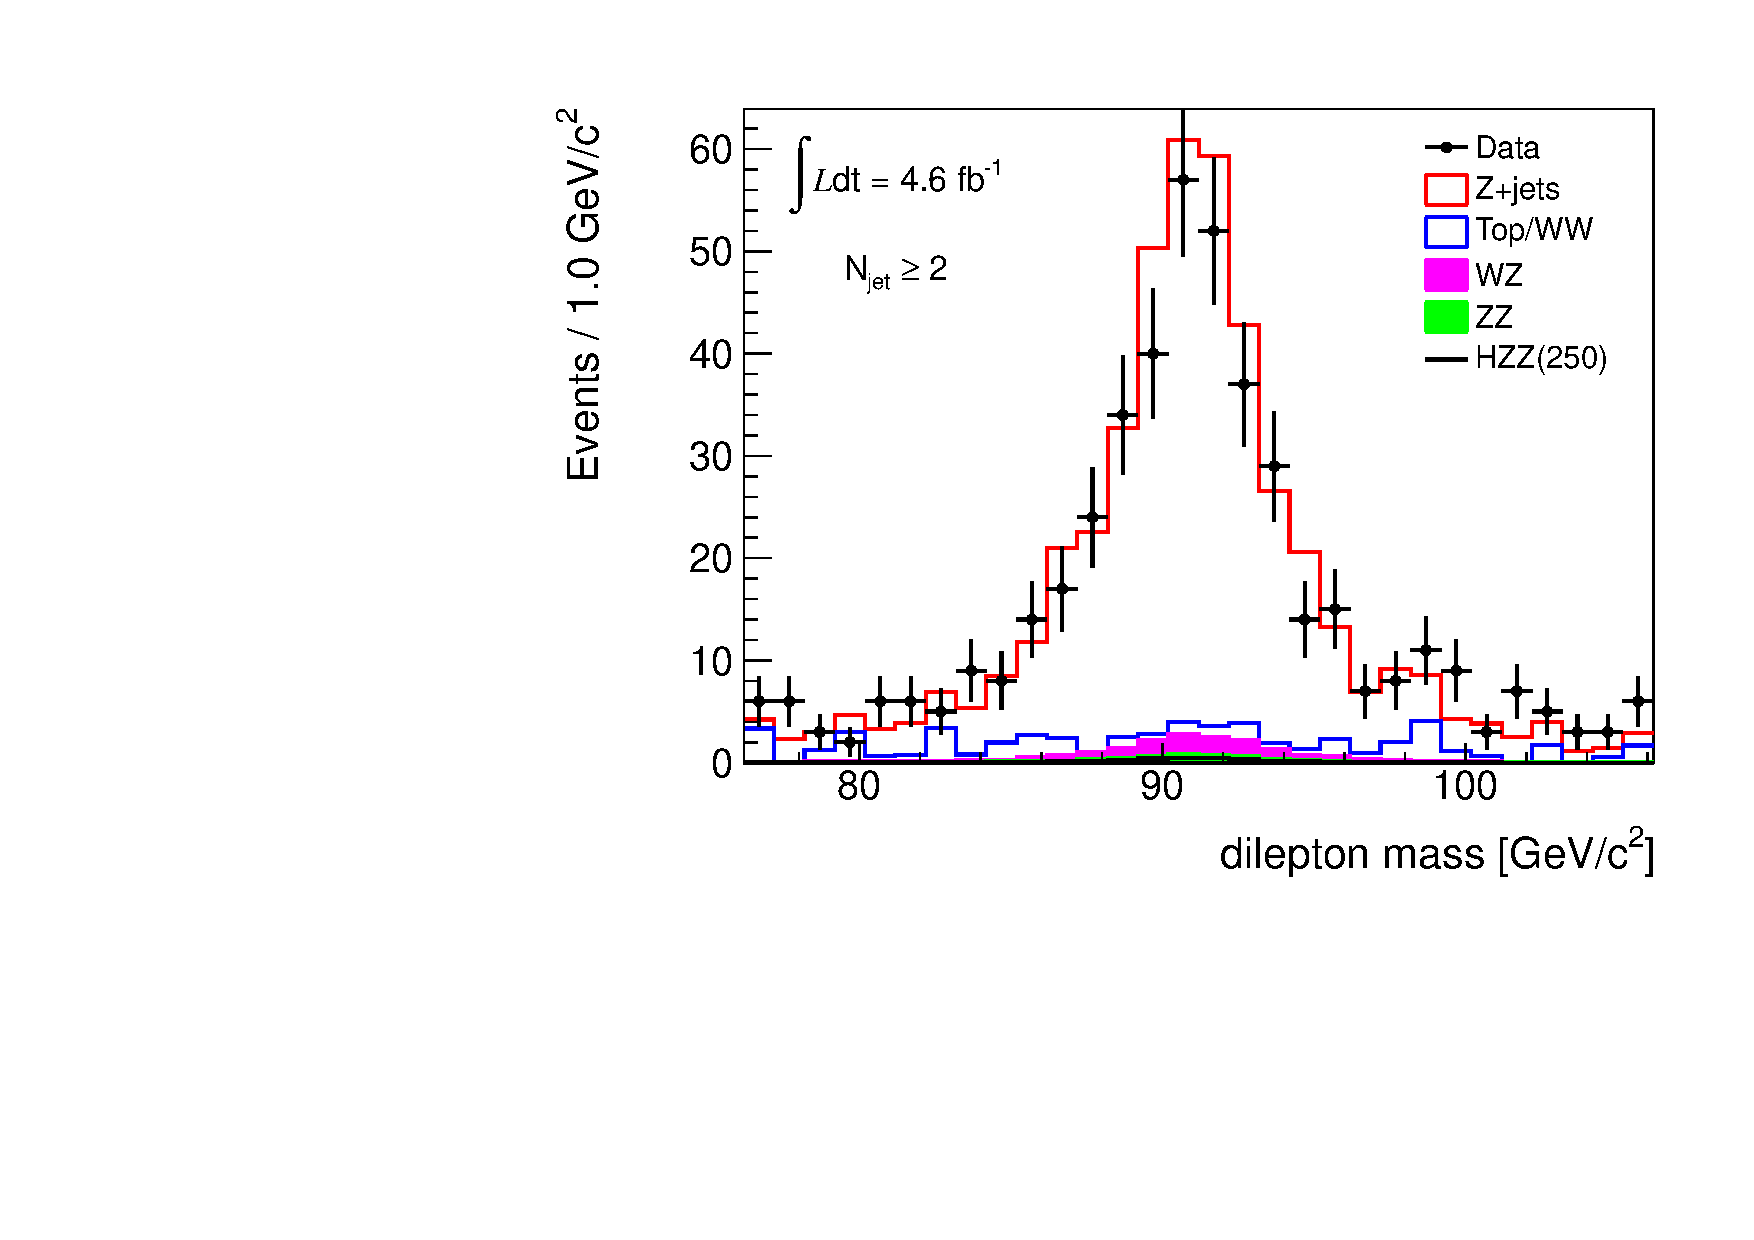
\includegraphics[width=.4\textwidth]{figures/presel_mH250_mm_mass_2j.pdf}}
\caption{Dilepton mass distribution in the muon channel after the $\ZZ$ preselection observed in data corresponding to $2.1$~\ifb data in 
the Inclusive~\subref{subfig:zmass_mm_incl}, 0-Jet~\subref{subfig:zmass_mm_0j}, 1-Jet~\subref{subfig:zmass_mm_1j} and 2-Jet~\subref{subfig:zmass_mm_2j} bins, 
compared to the expected from simulation for signal and background. The MC backgrounds are scaled as appropriate and the photon+jets estimate of the 
Z+jets background is added to the stack.}
\label{fig:zmass_zzpresel_mm}
\end{center}
\end{figure}
%%%%%%%%

%%%%%%%%
\begin{figure}[!hbtp]
\begin{center}
\subfigure[Inclusive]{\label{subfig:zmass_ee_incl}
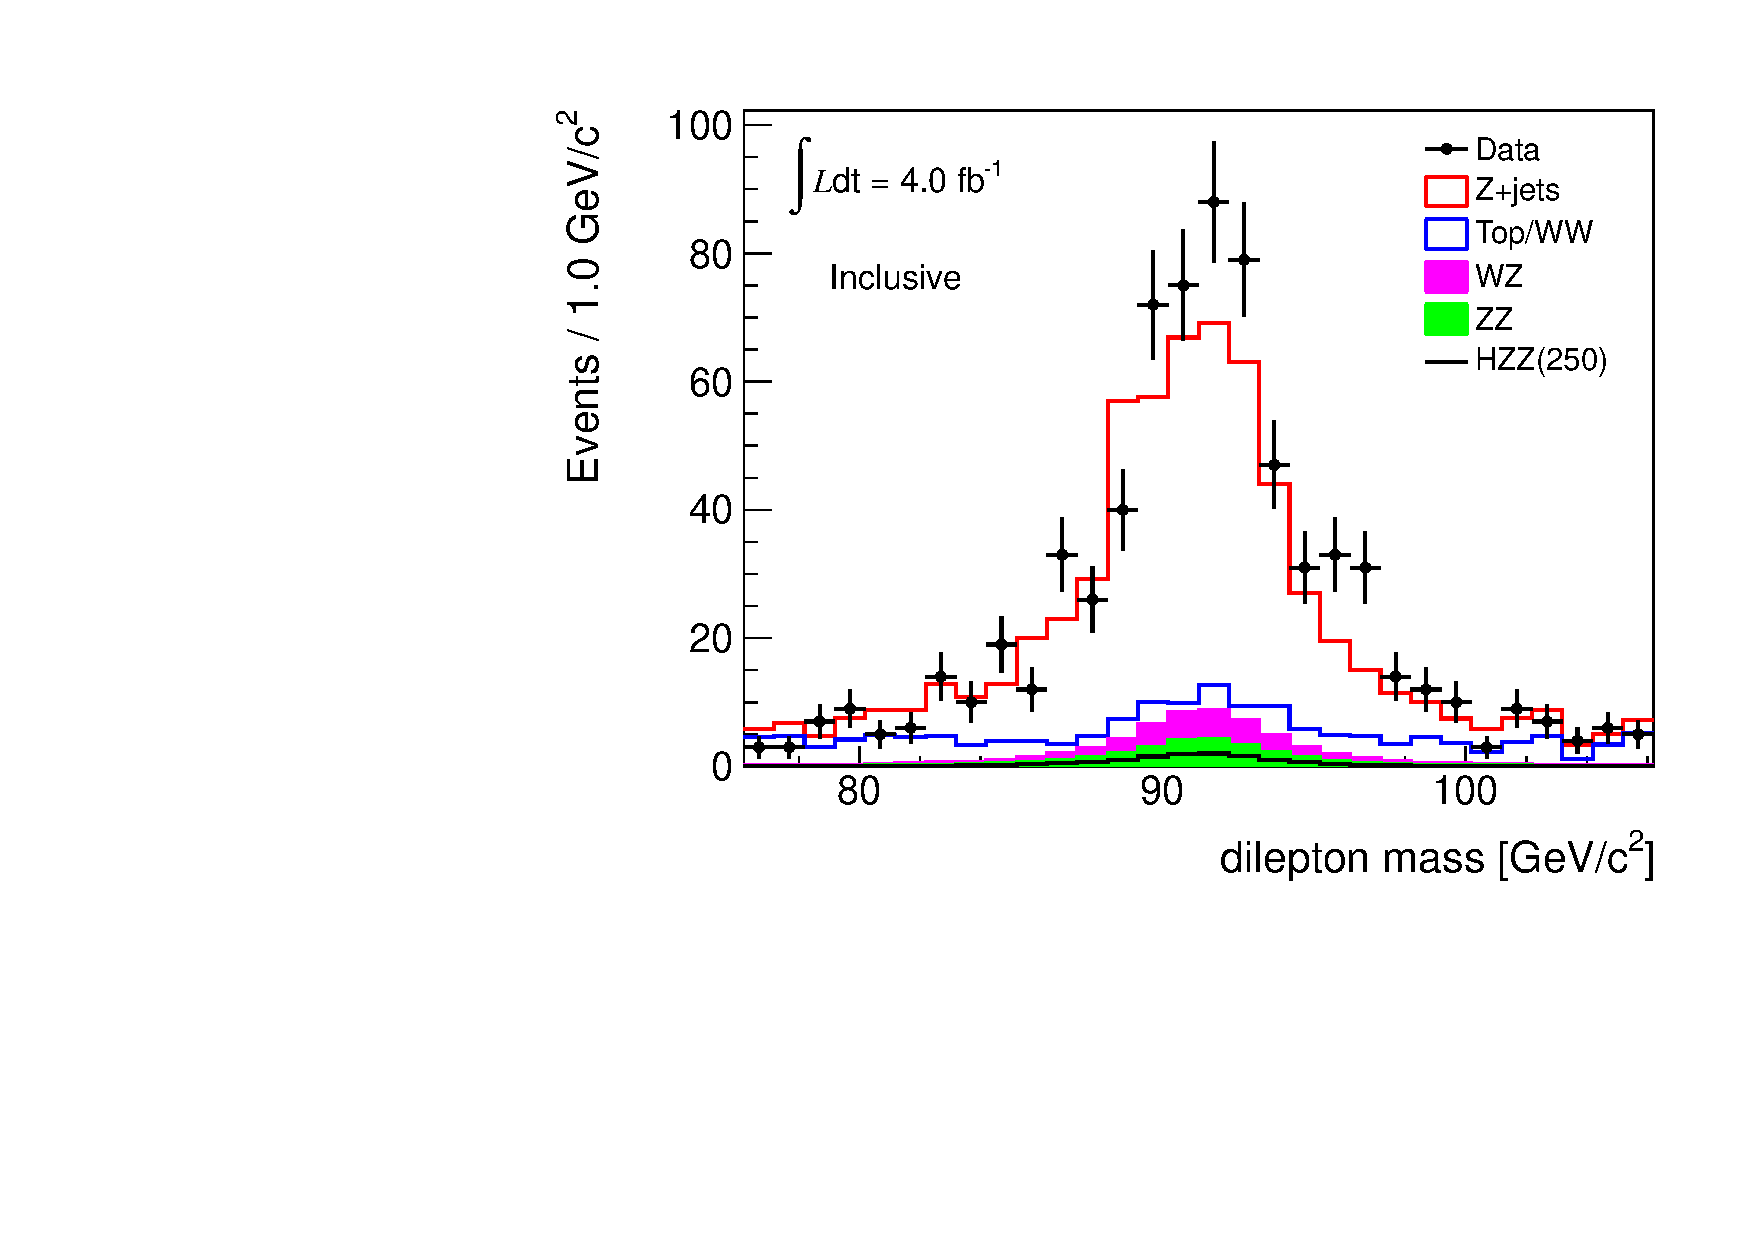
\includegraphics[width=.4\textwidth]{figures/presel_mH250_ee_mass_incl.pdf}}
\subfigure[0-Jet]{\label{subfig:zmass_ee_0j}
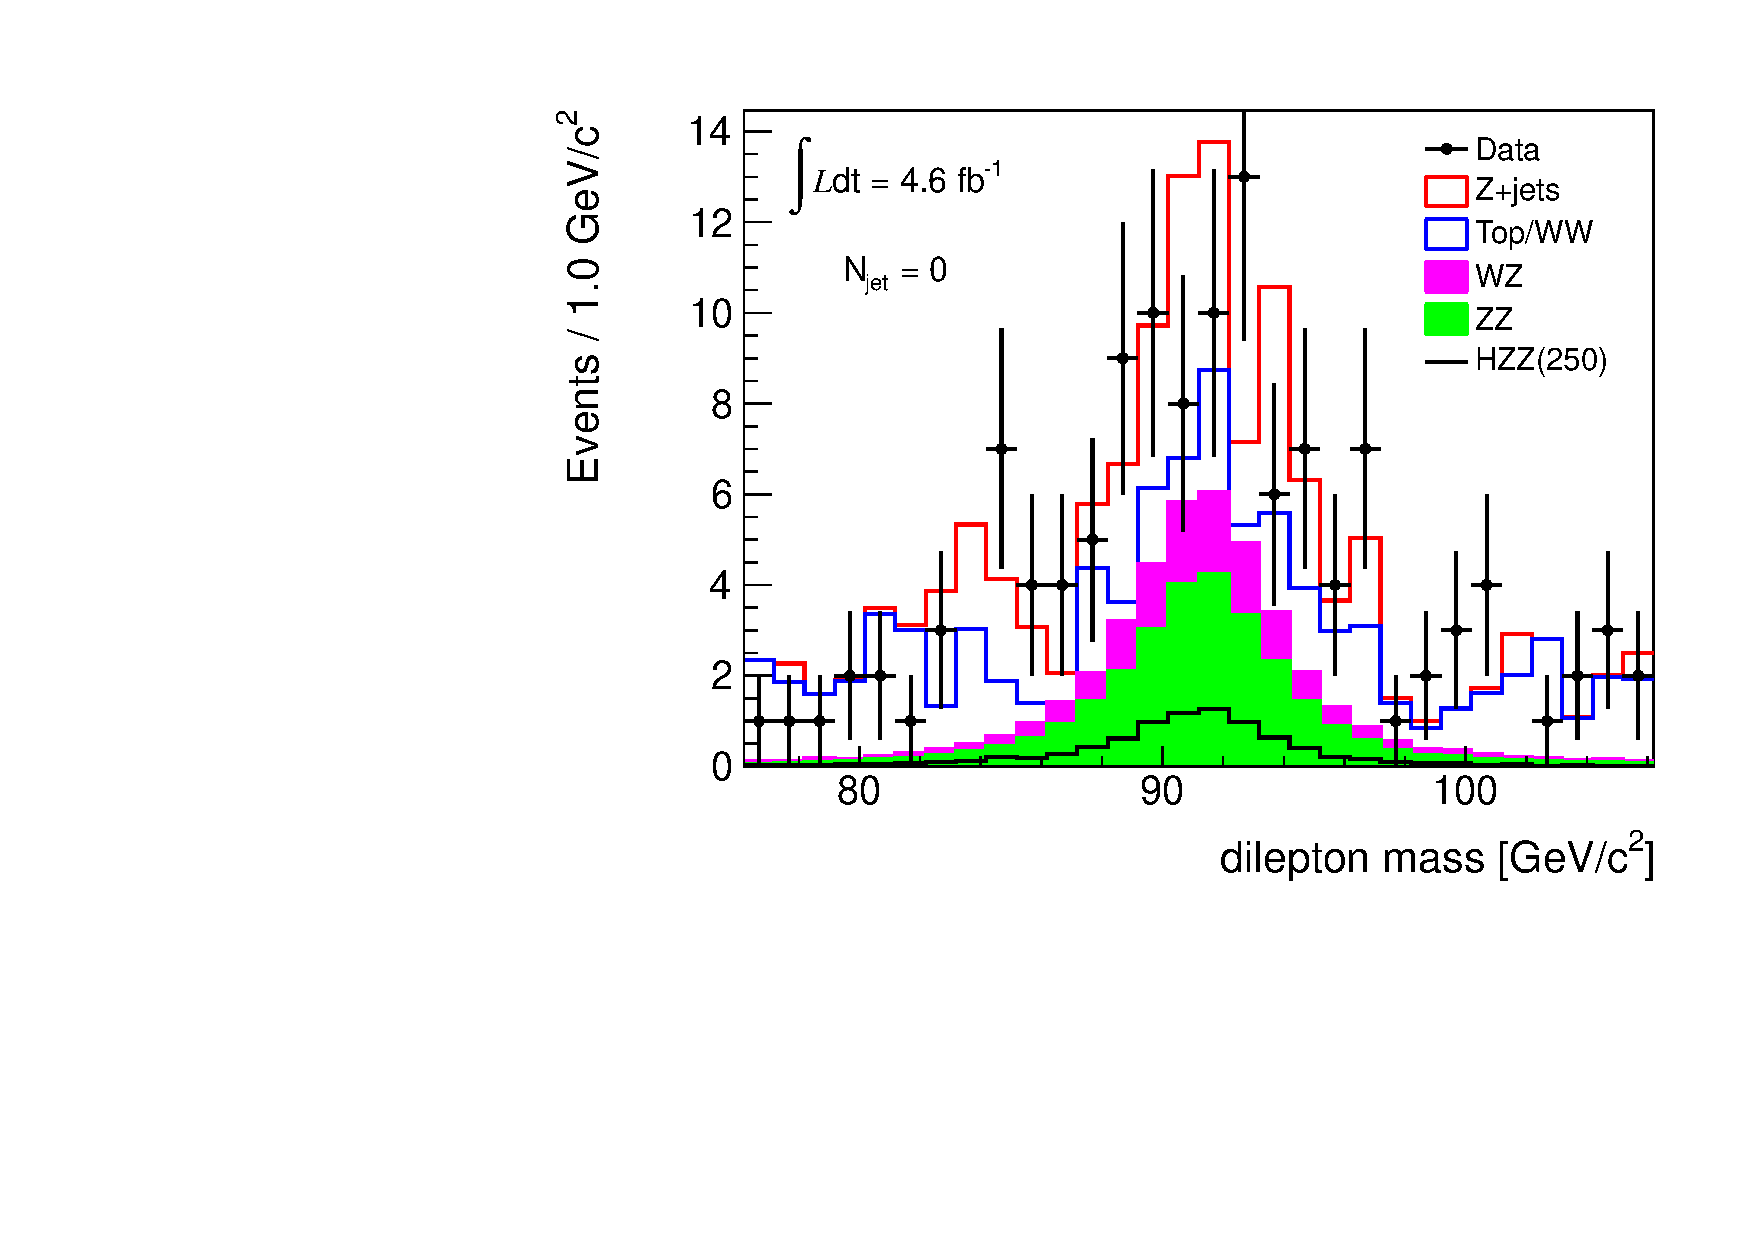
\includegraphics[width=.4\textwidth]{figures/presel_mH250_ee_mass_0j.pdf}} \\
\subfigure[1-Jet]{\label{subfig:zmass_ee_1j}
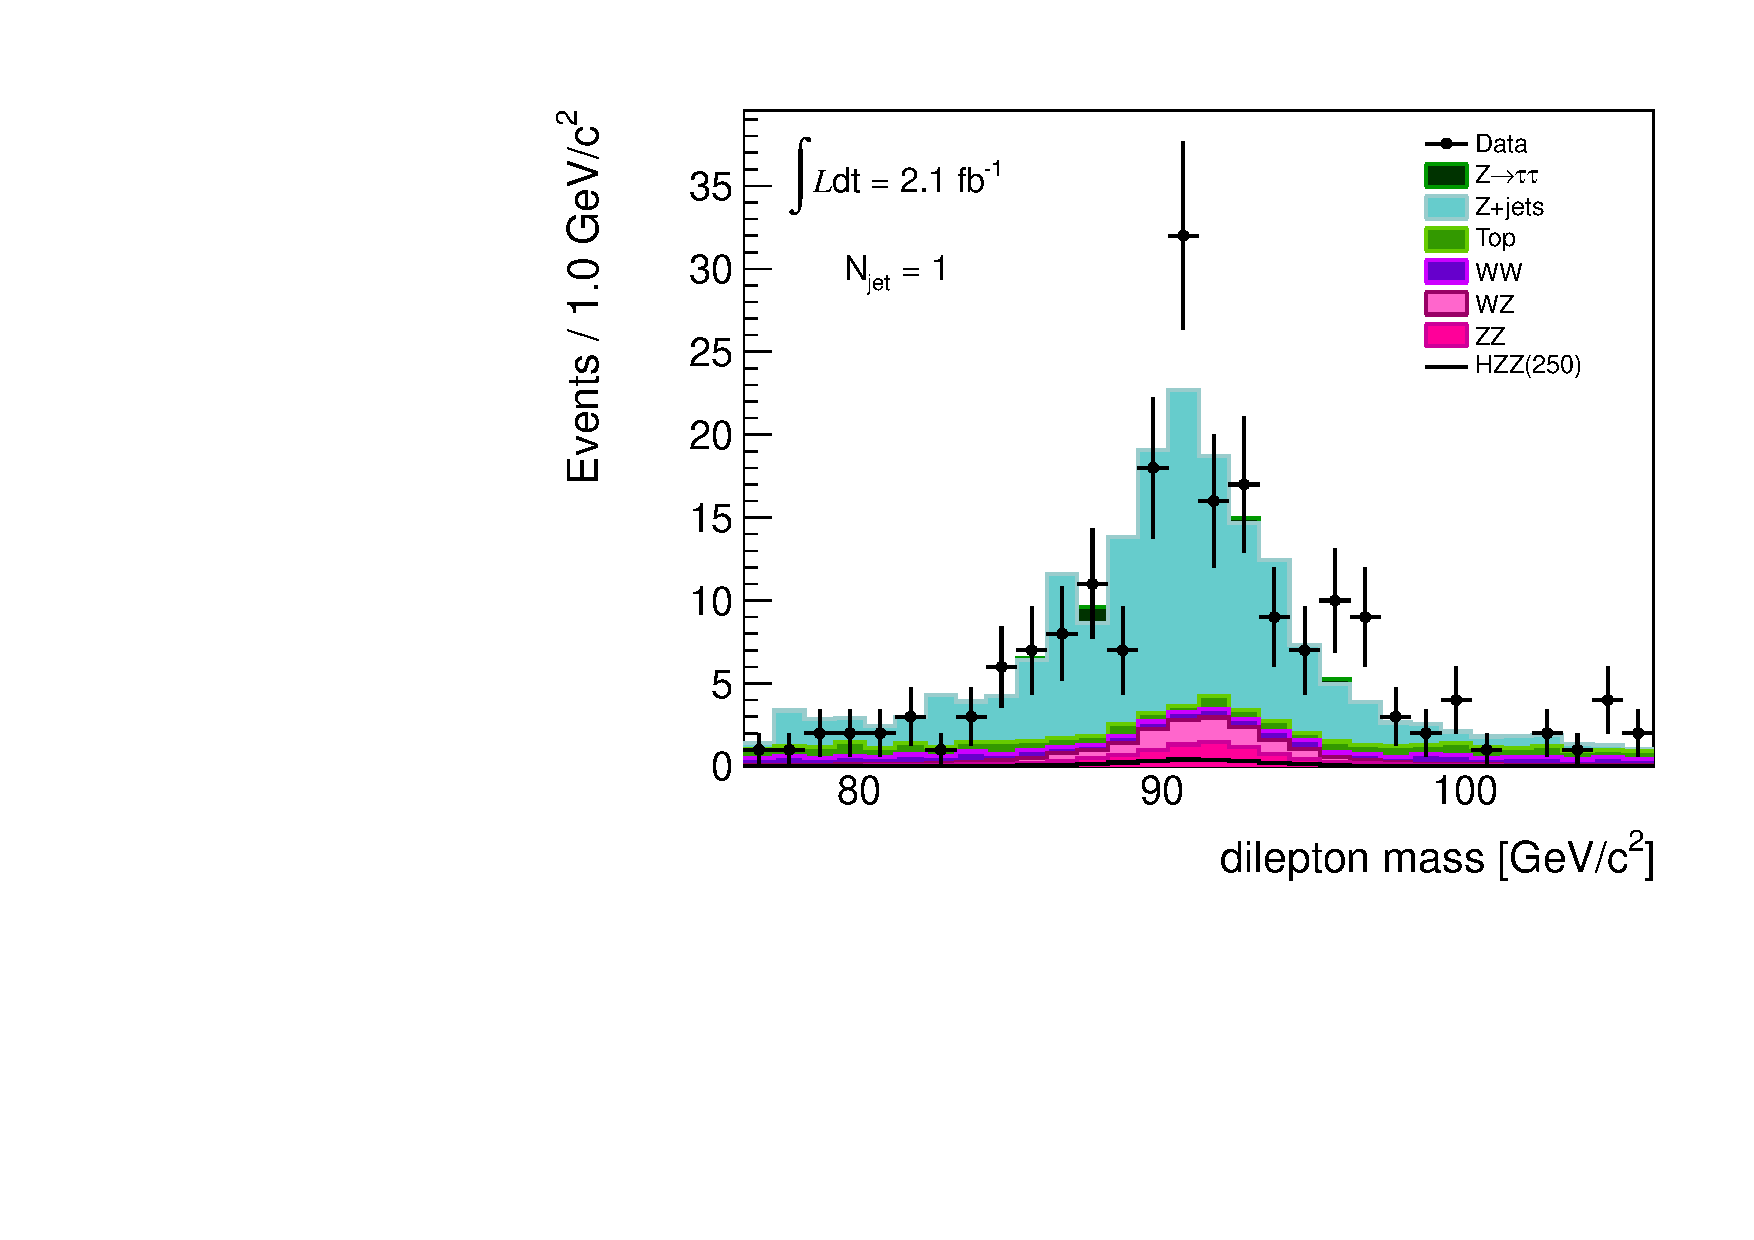
\includegraphics[width=.4\textwidth]{figures/presel_mH250_ee_mass_1j.pdf}}
\subfigure[$\geq$2 Jets]{\label{subfig:zmass_ee_2j}
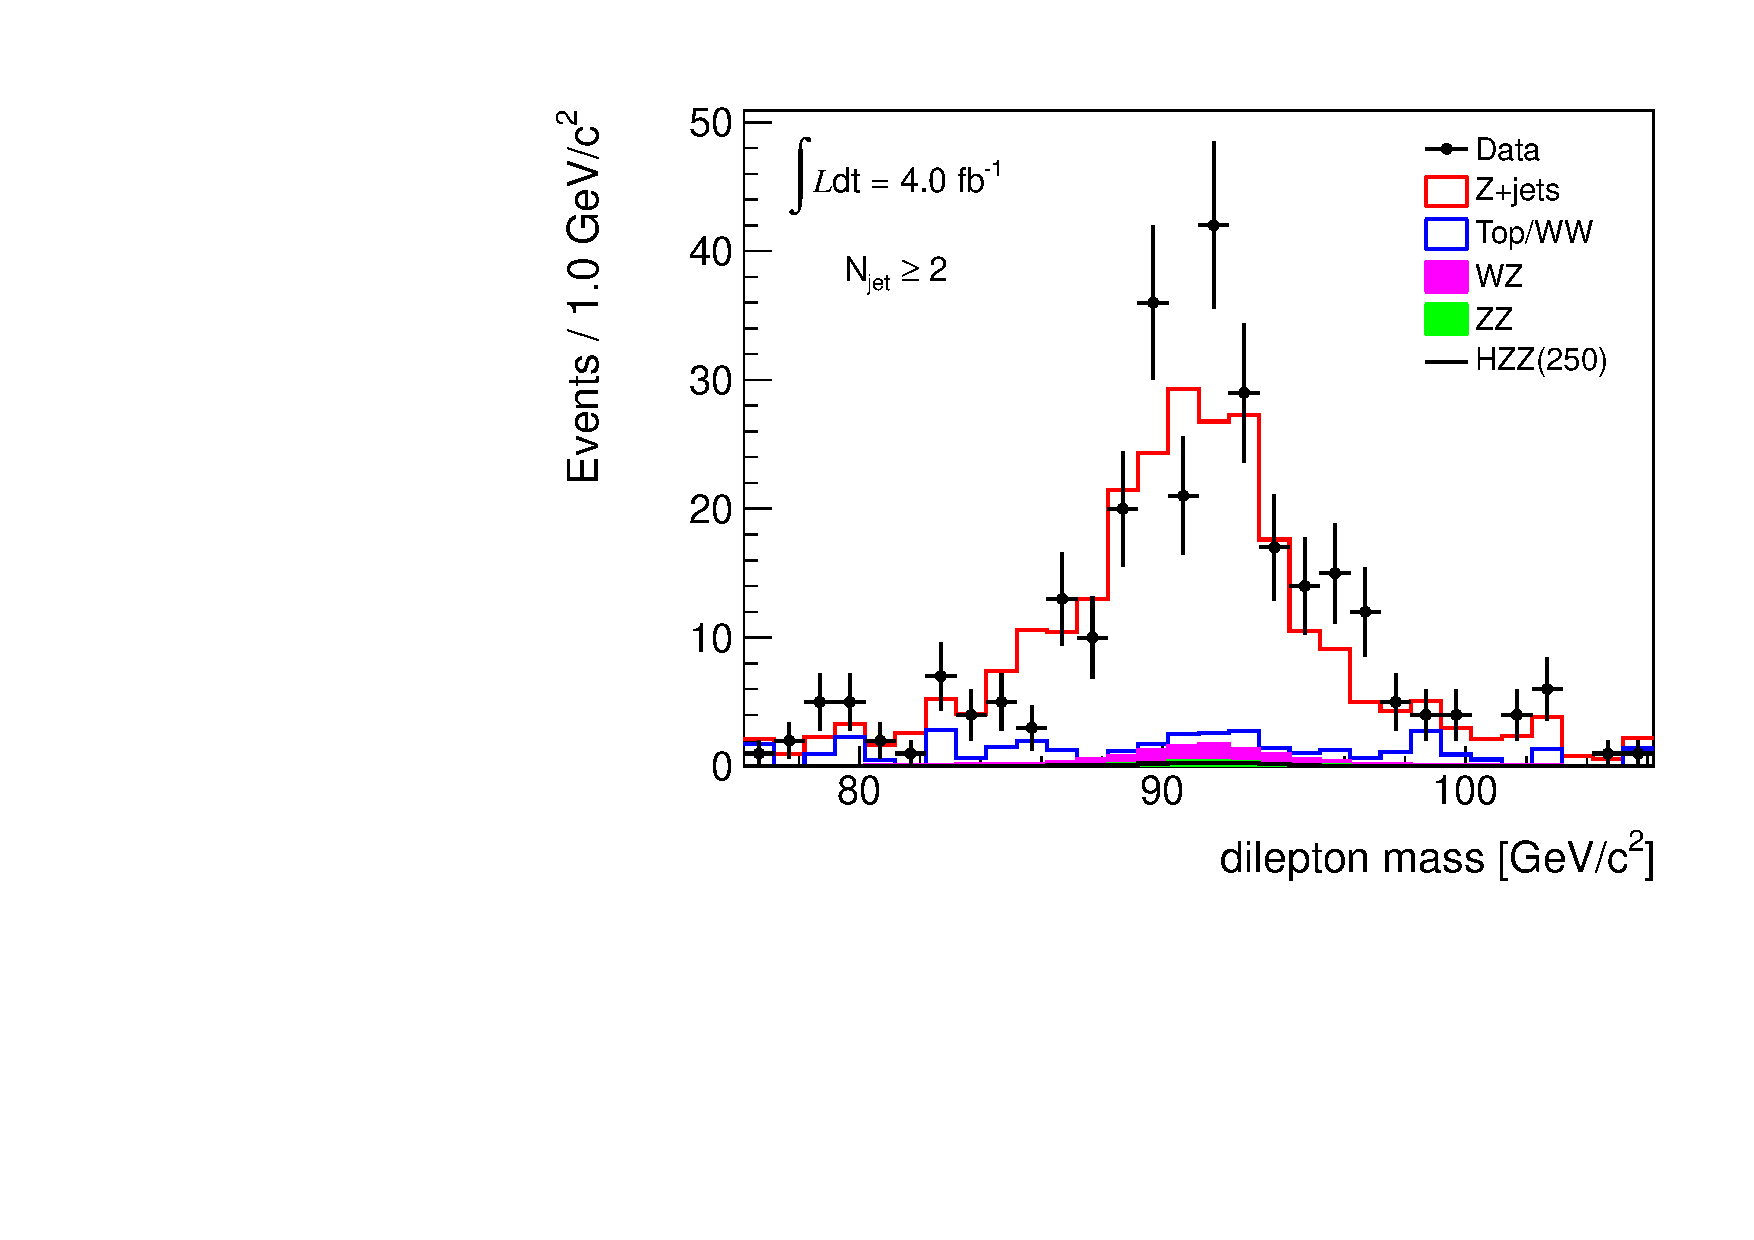
\includegraphics[width=.4\textwidth]{figures/presel_mH250_ee_mass_2j.pdf}}
\caption{Dilepton mass distribution in the electron channel after the $\ZZ$ preselection observed in data corresponding to $2.1$~\ifb data in 
the Inclusive~\subref{subfig:zmass_ee_incl}, 0-Jet~\subref{subfig:zmass_ee_0j}, 1-Jet~\subref{subfig:zmass_ee_1j} and 2-Jet~\subref{subfig:zmass_ee_2j} bins, 
compared to the expected from simulation for signal and background. The MC backgrounds are scaled as appropriate and the photon+jets estimate of the 
Z+jets background is added to the stack.}
\label{fig:zmass_zzpresel_ee}
\end{center}
\end{figure}
%%%%%%%%

%%%%%%%%
\begin{figure}[!hbtp]
\begin{center}
\subfigure[Inclusive]{\label{subfig:zpt_mm_incl}
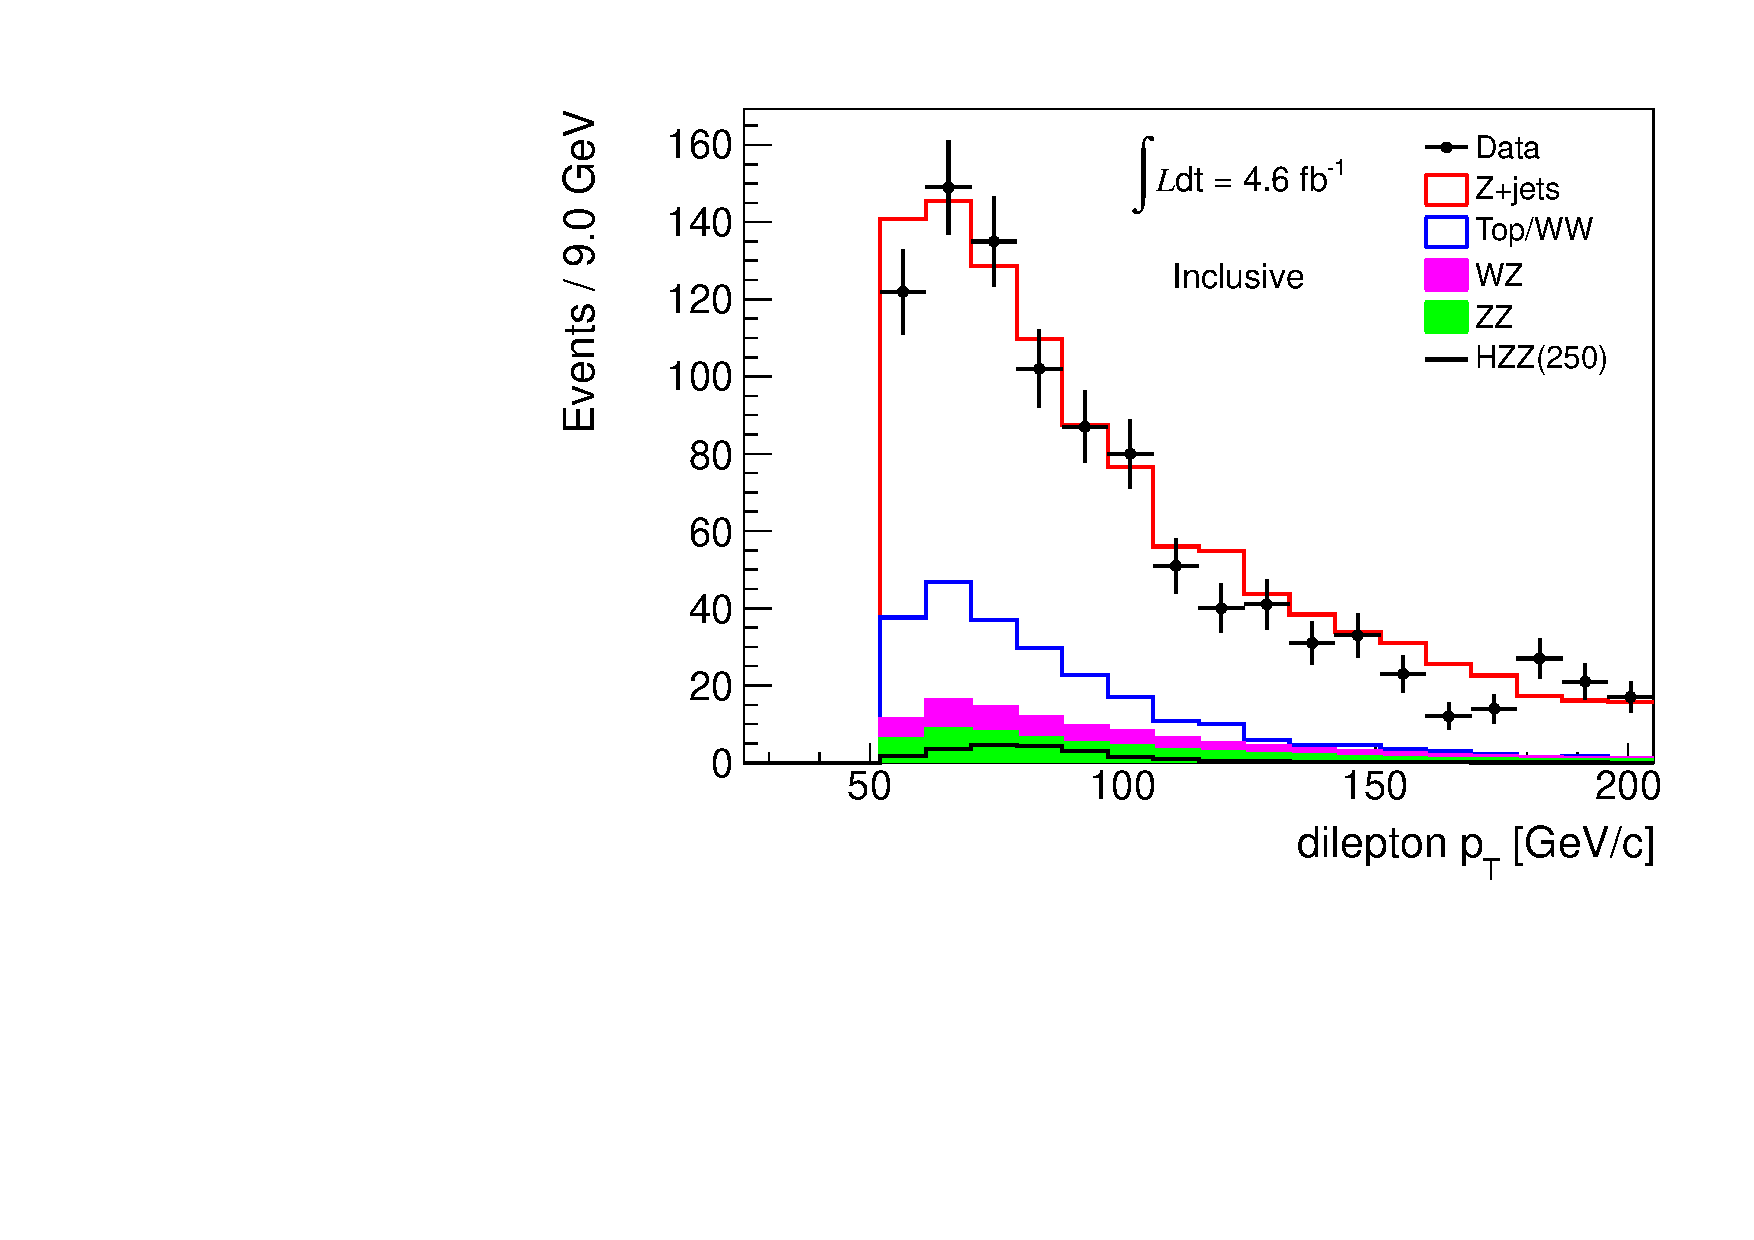
\includegraphics[width=.4\textwidth]{figures/presel_mH250_mm_dileppt_incl.pdf}}
\subfigure[0-Jet]{\label{subfig:zpt_mm_0j}
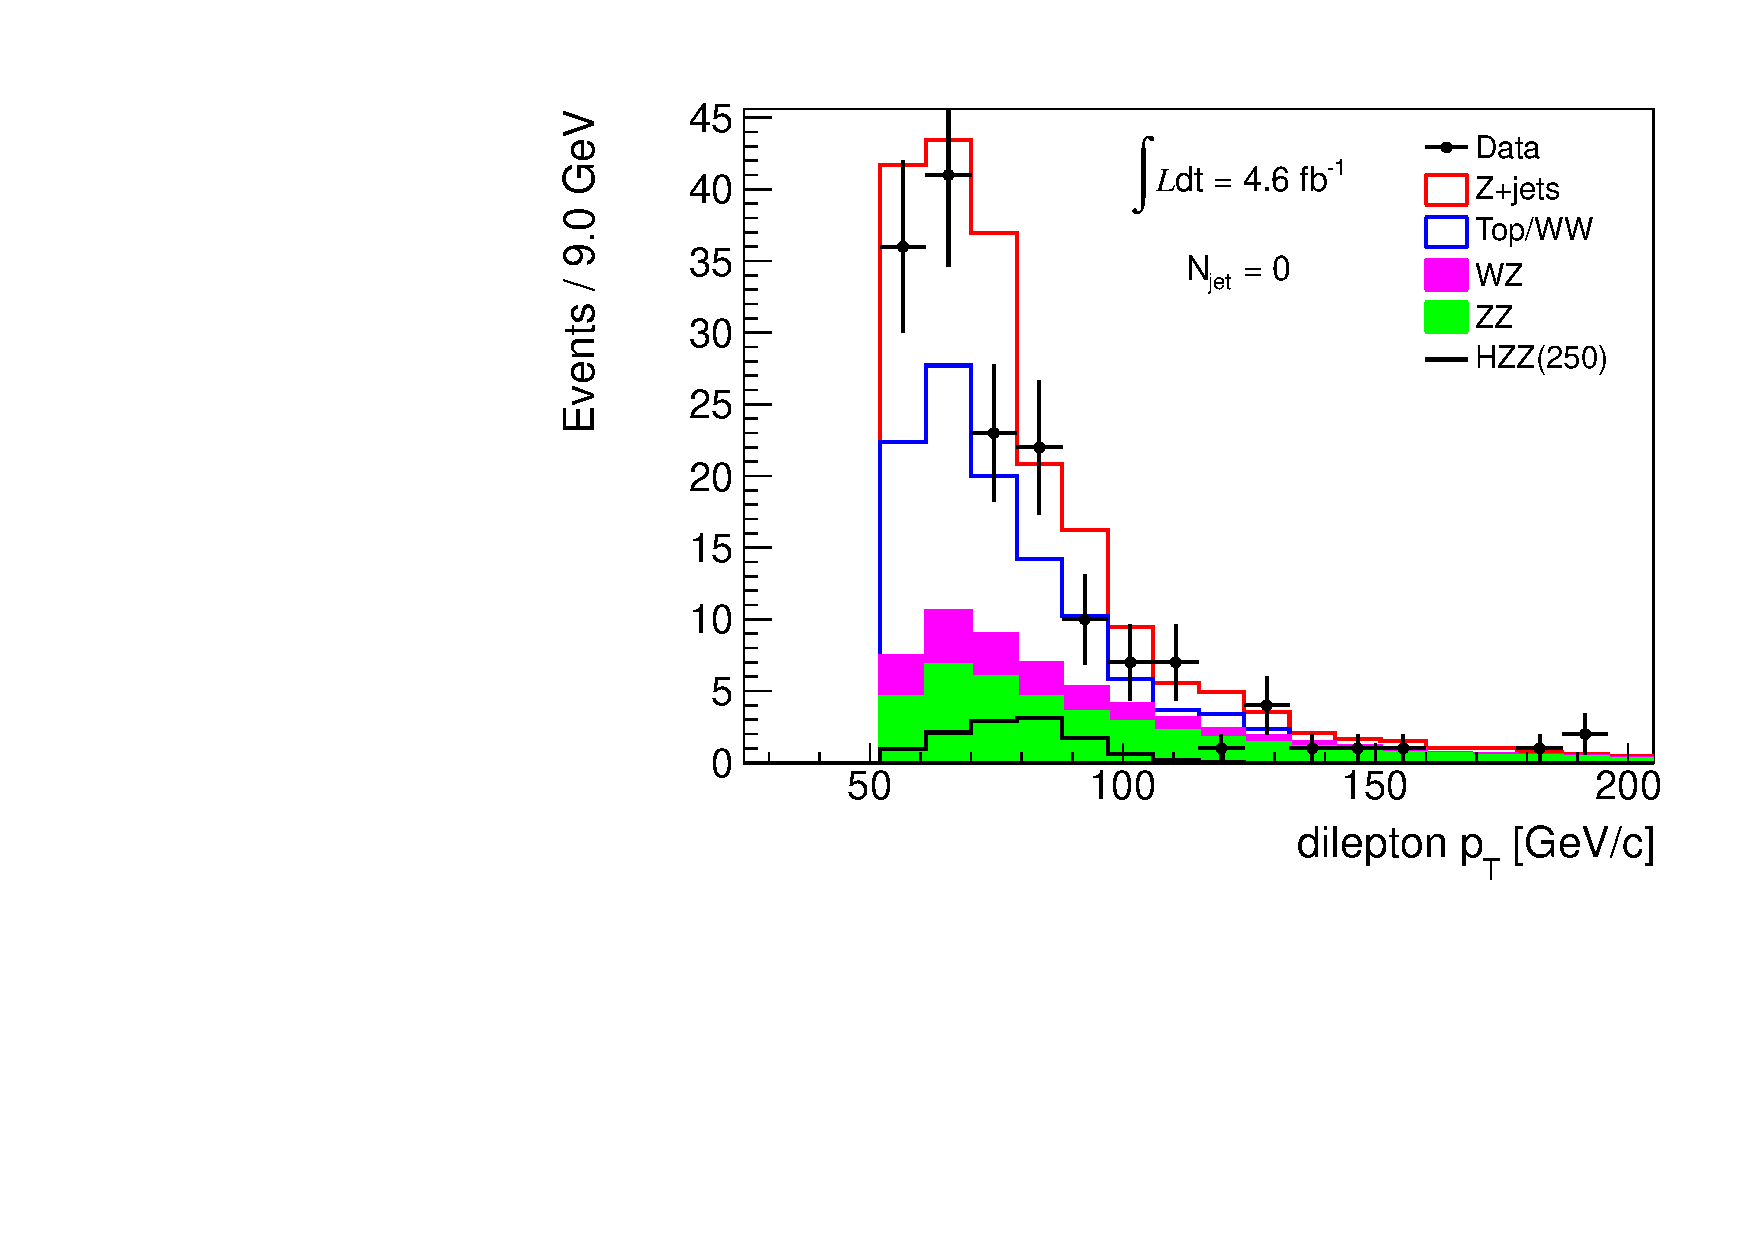
\includegraphics[width=.4\textwidth]{figures/presel_mH250_mm_dileppt_0j.pdf}} \\
\subfigure[1-Jet]{\label{subfig:zpt_mm_1j}
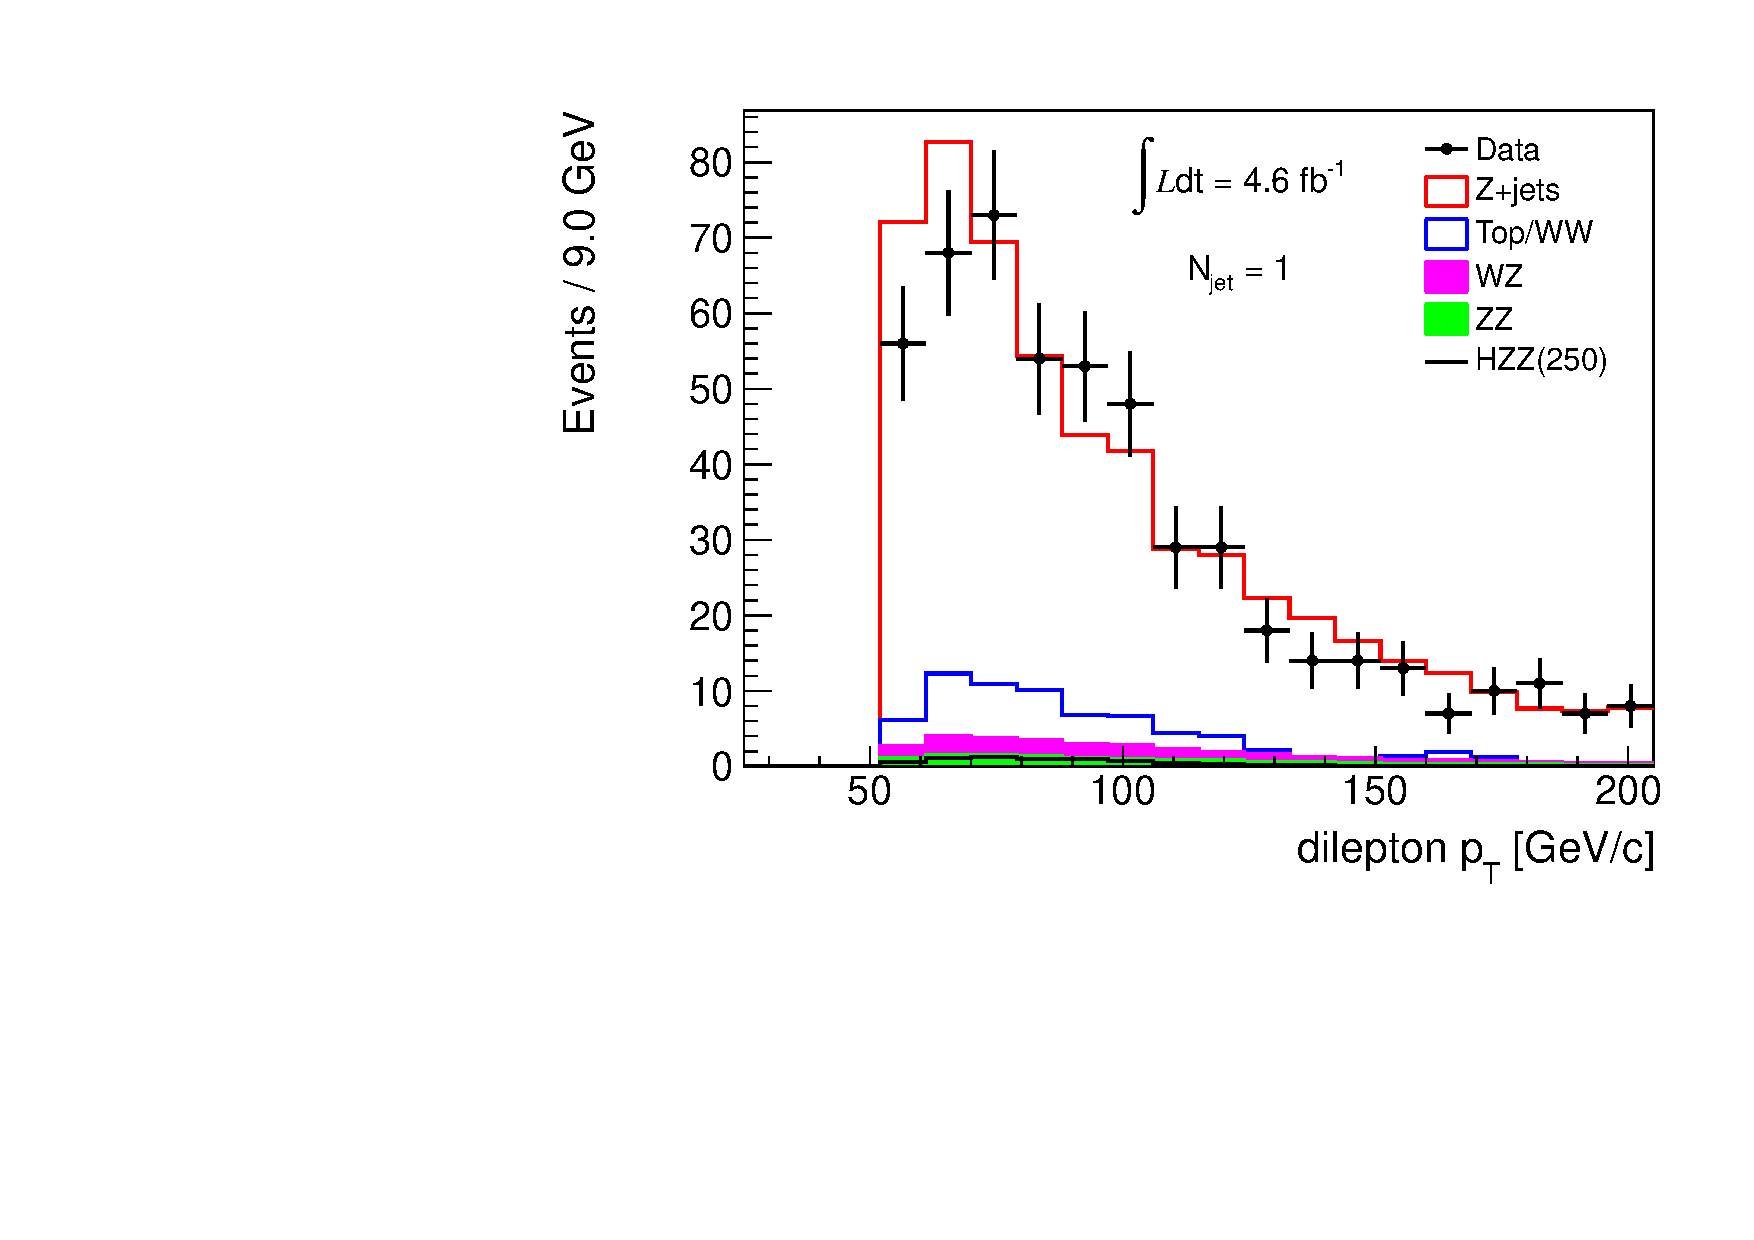
\includegraphics[width=.4\textwidth]{figures/presel_mH250_mm_dileppt_1j.pdf}}
\subfigure[$\geq$2 Jets]{\label{subfig:zpt_mm_2j}
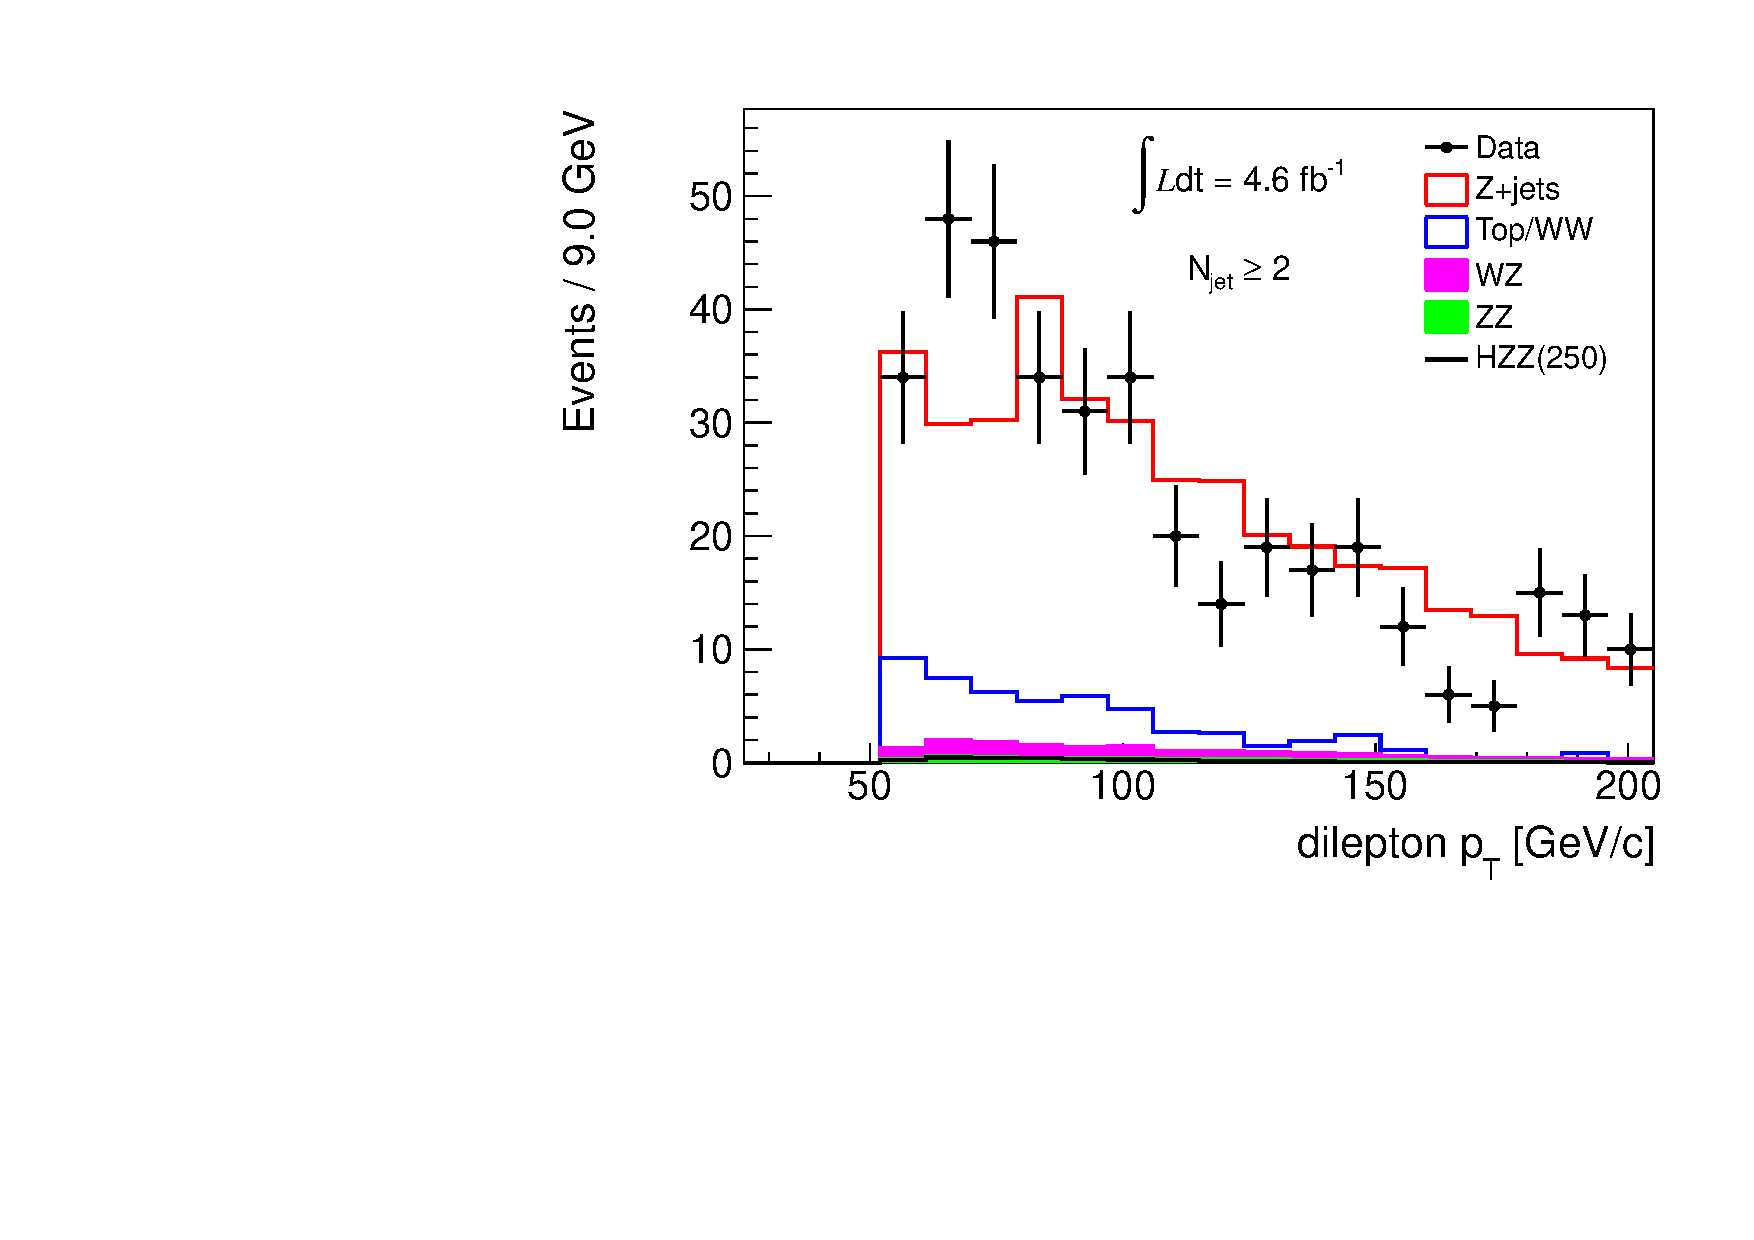
\includegraphics[width=.4\textwidth]{figures/presel_mH250_mm_dileppt_2j.pdf}}
\caption{Dilepton $p_T$ distribution in the muon channel after the $\ZZ$ preselection observed in data corresponding to $2.1$~\ifb data in 
the Inclusive~\subref{subfig:zpt_mm_incl}, 0-Jet~\subref{subfig:zpt_mm_0j}, 1-Jet~\subref{subfig:zpt_mm_1j} and 2-Jet~\subref{subfig:zpt_mm_2j} bins, 
compared to the expected from simulation for signal and background. The MC backgrounds are scaled as appropriate and the photon+jets estimate of the 
Z+jets background is added to the stack.}
\label{fig:zpt_zzpresel_mm}
\end{center}
\end{figure}
%%%%%%%%

%%%%%%%%
\begin{figure}[!hbtp]
\begin{center}
\subfigure[Inclusive]{\label{subfig:zpt_ee_incl}
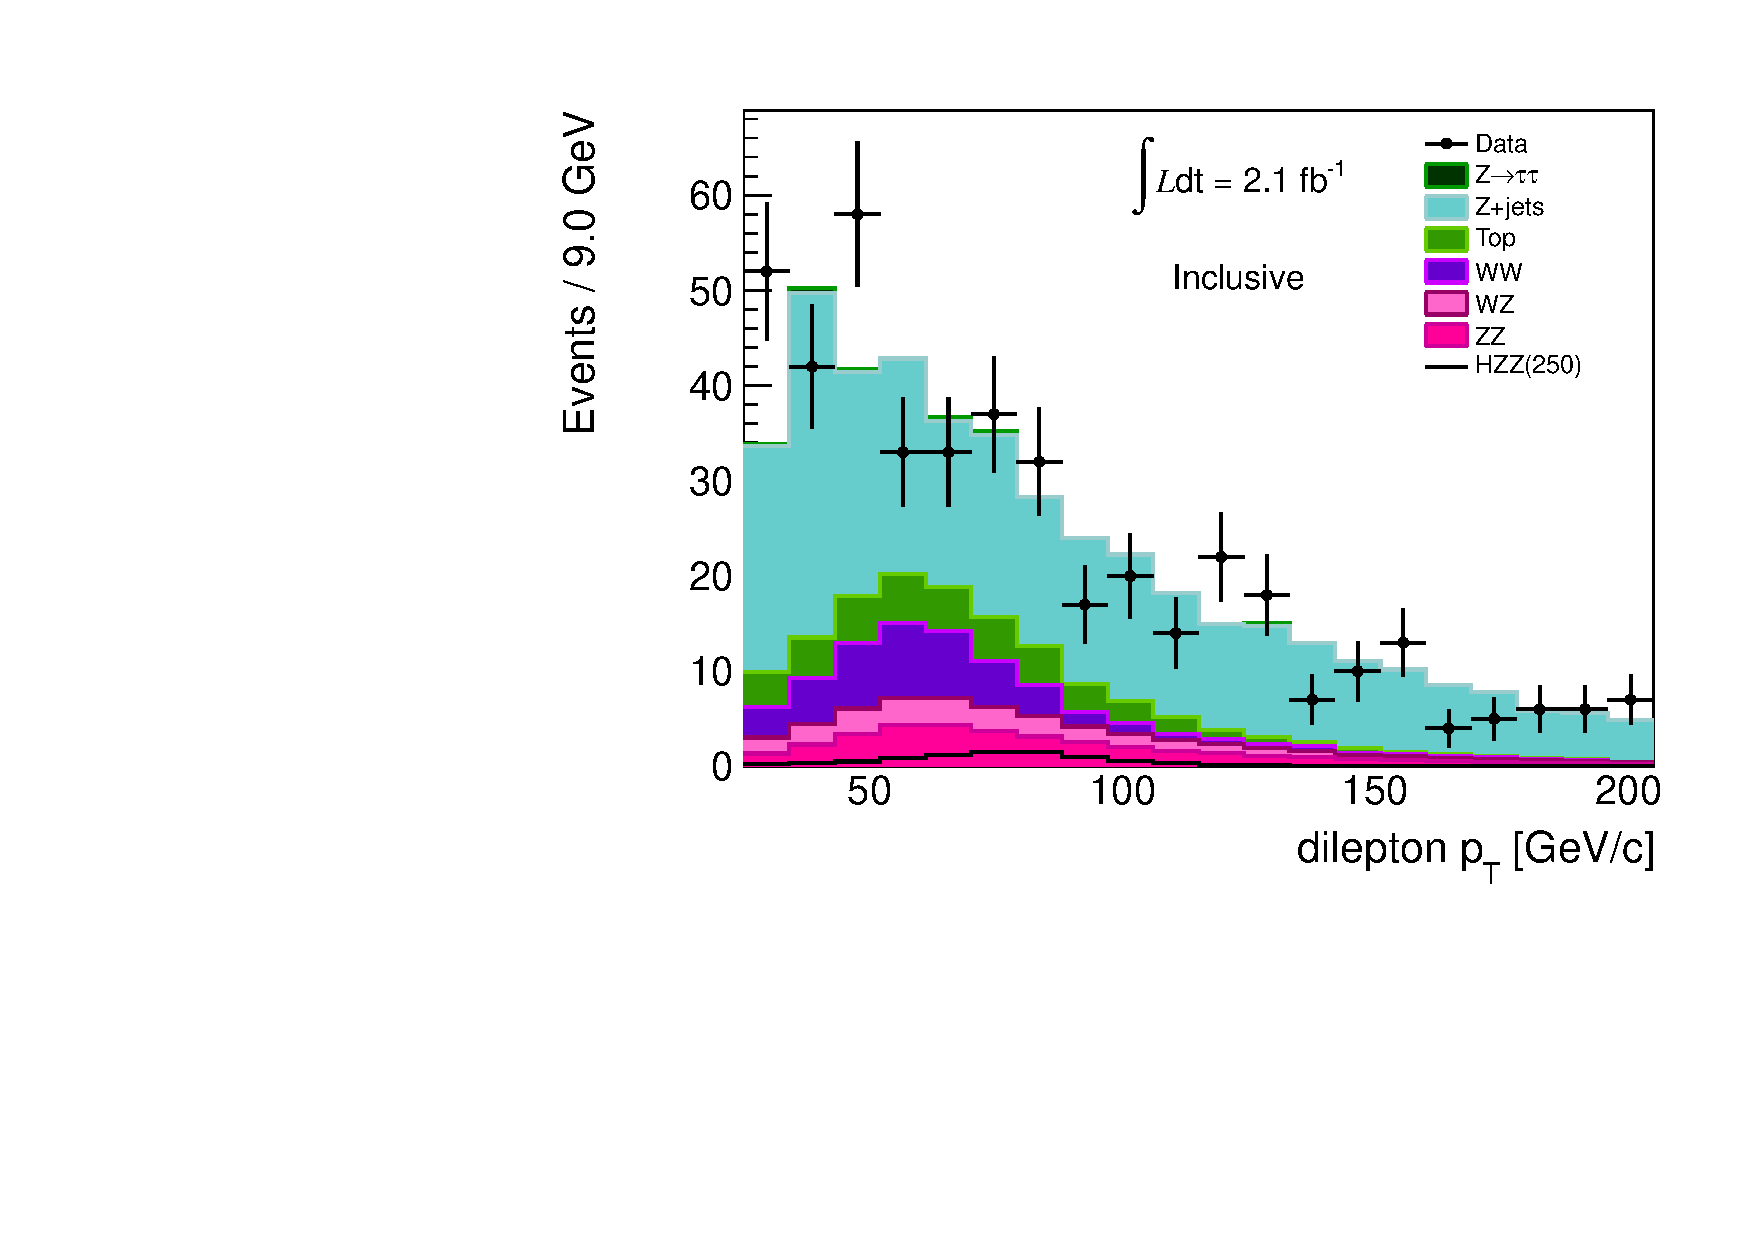
\includegraphics[width=.4\textwidth]{figures/presel_mH250_ee_dileppt_incl.pdf}}
\subfigure[0-Jet]{\label{subfig:zpt_ee_0j}
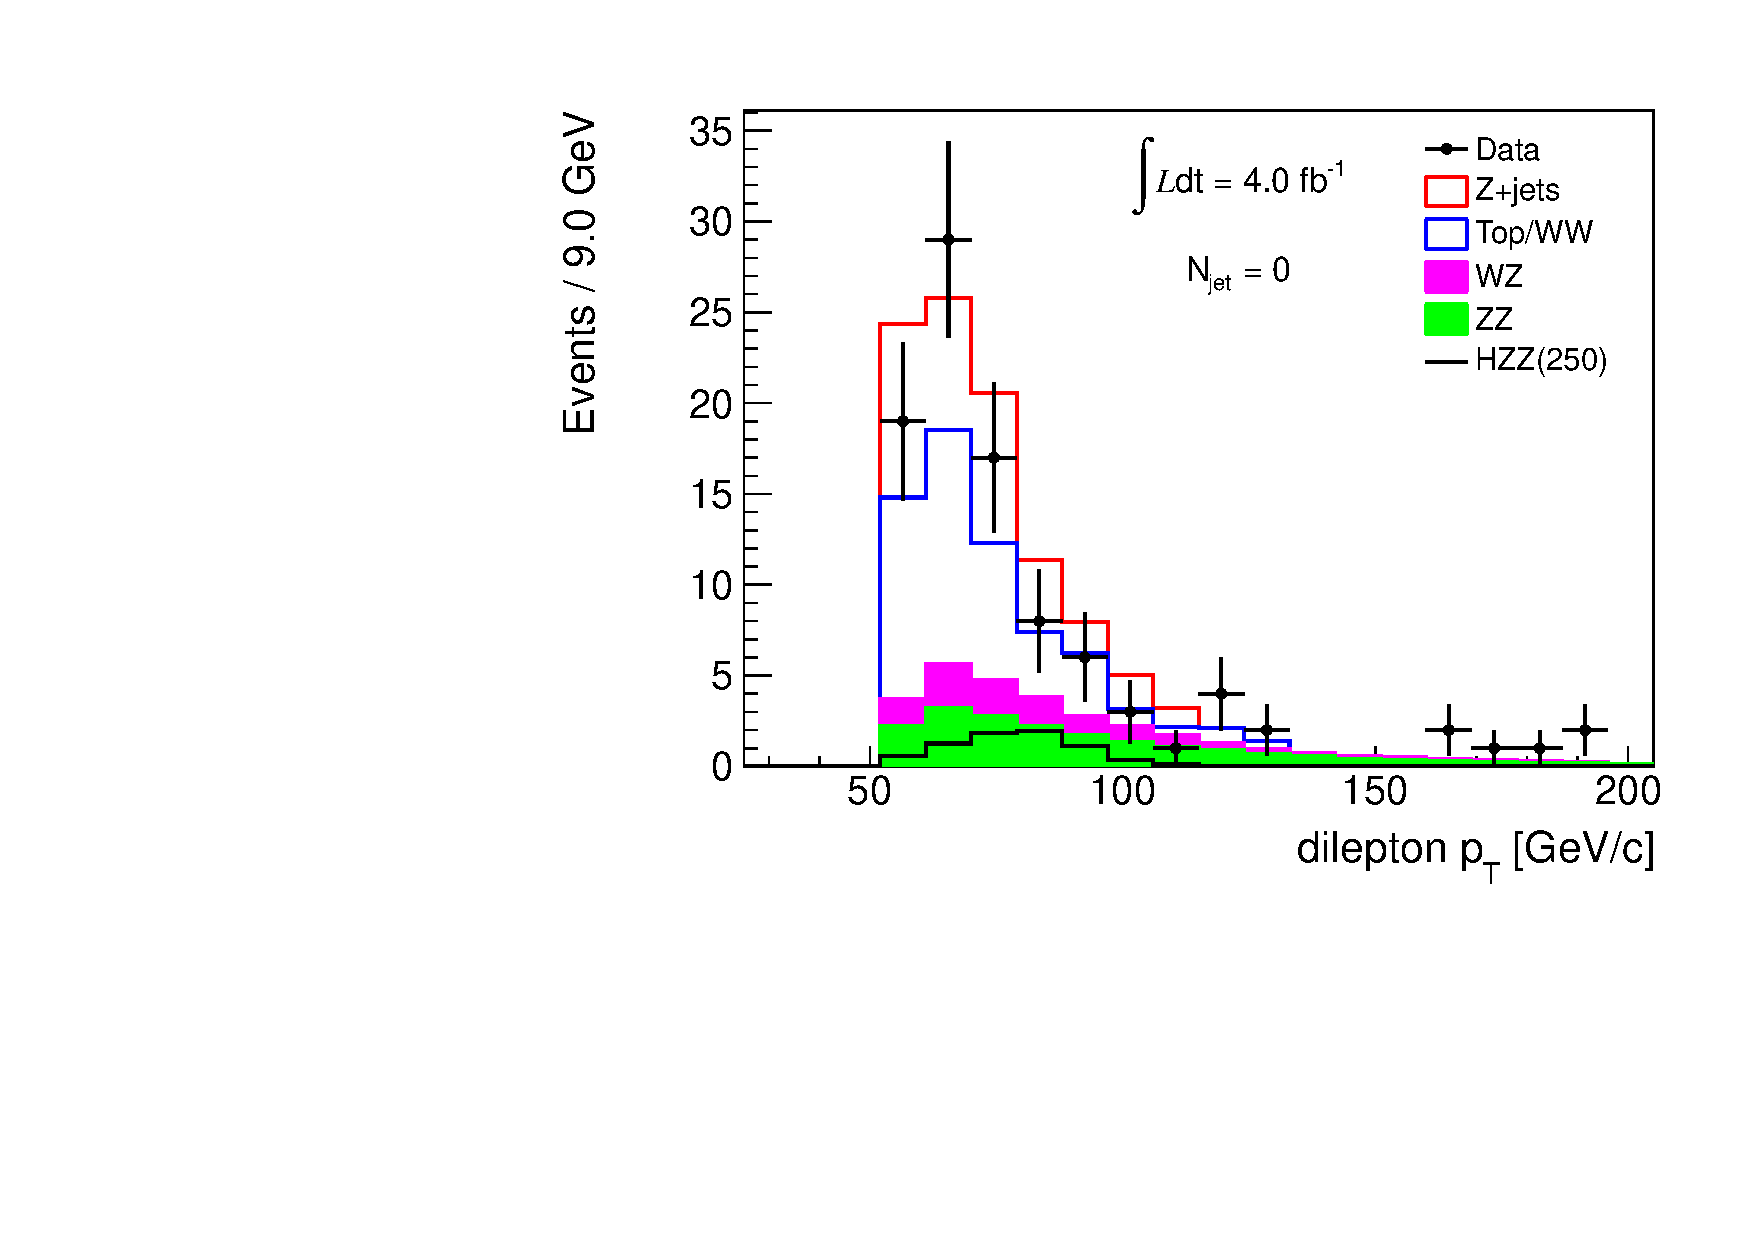
\includegraphics[width=.4\textwidth]{figures/presel_mH250_ee_dileppt_0j.pdf}} \\
\subfigure[1-Jet]{\label{subfig:zpt_ee_1j}
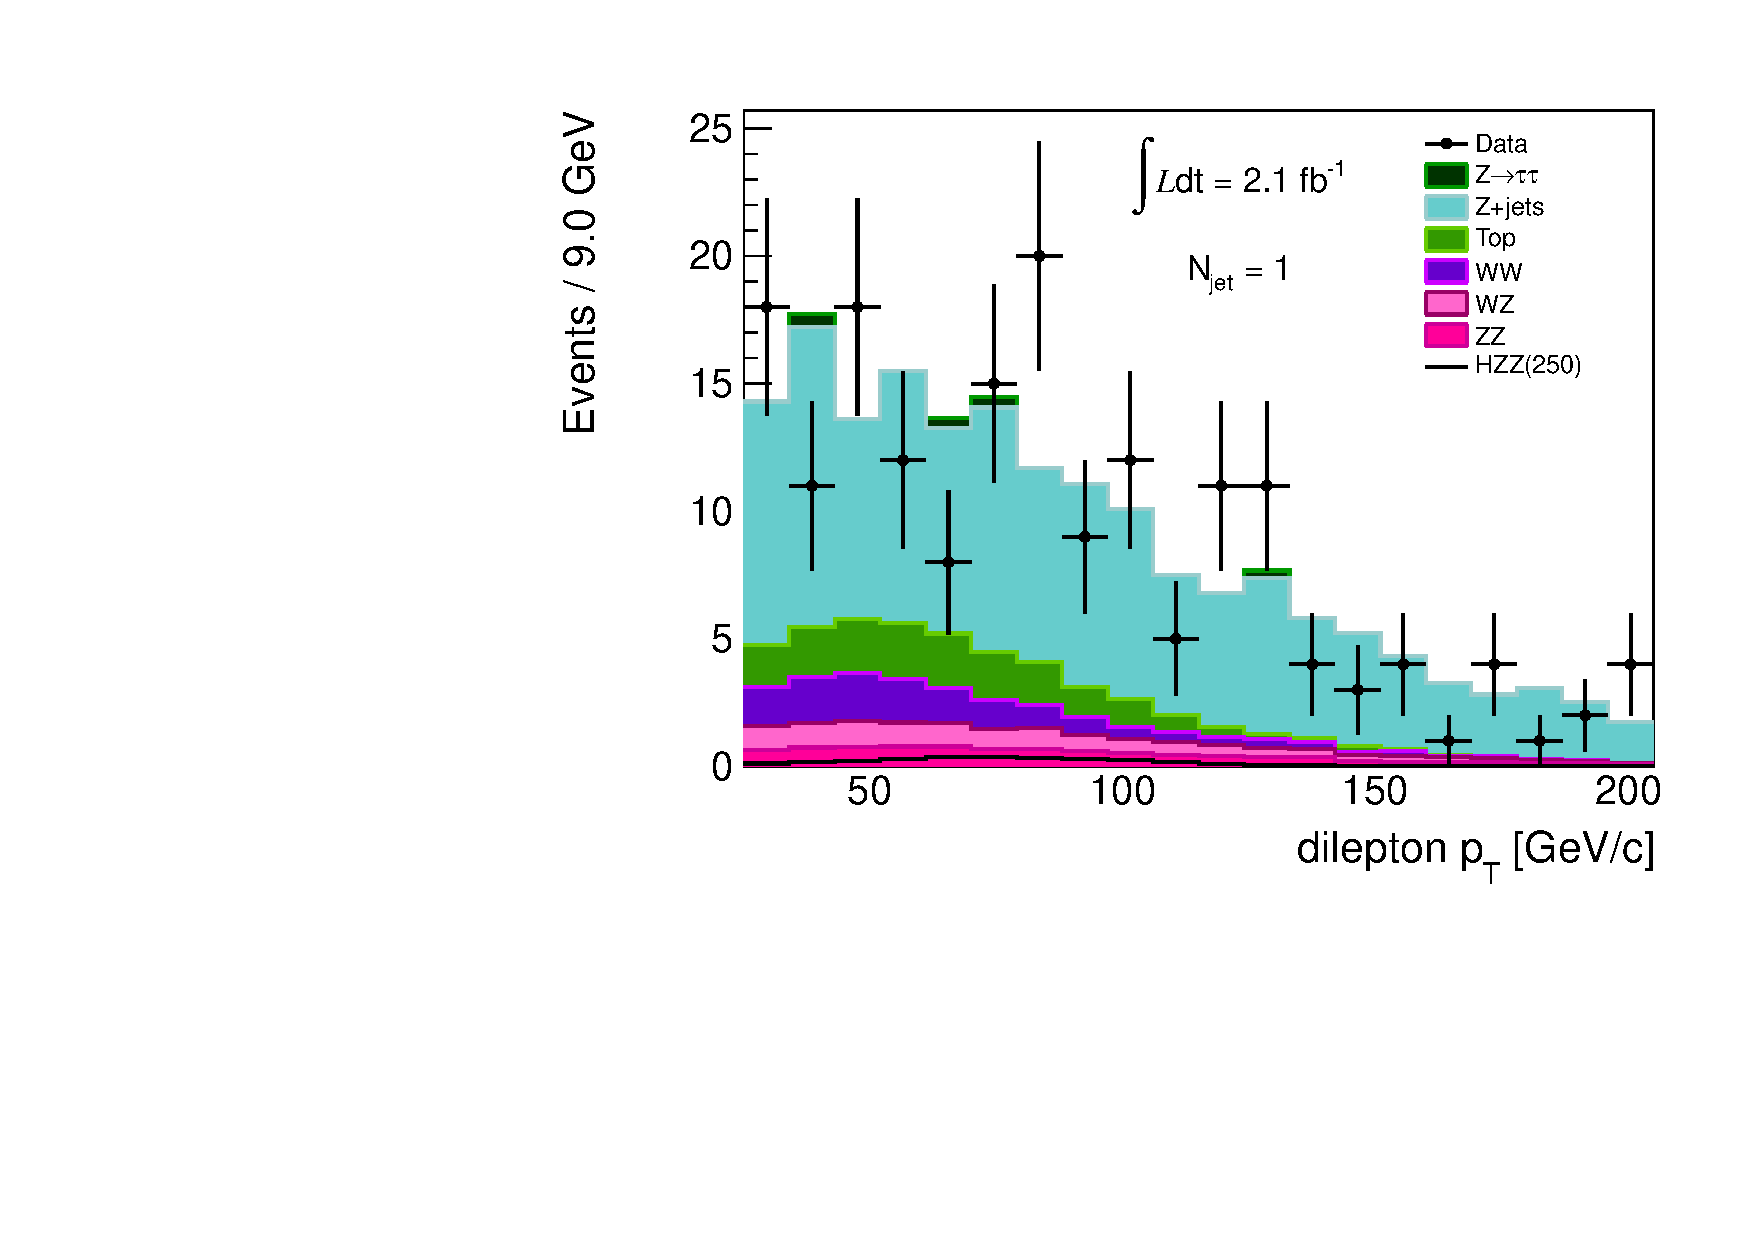
\includegraphics[width=.4\textwidth]{figures/presel_mH250_ee_dileppt_1j.pdf}}
\subfigure[$\geq$2 Jets]{\label{subfig:zpt_ee_2j}
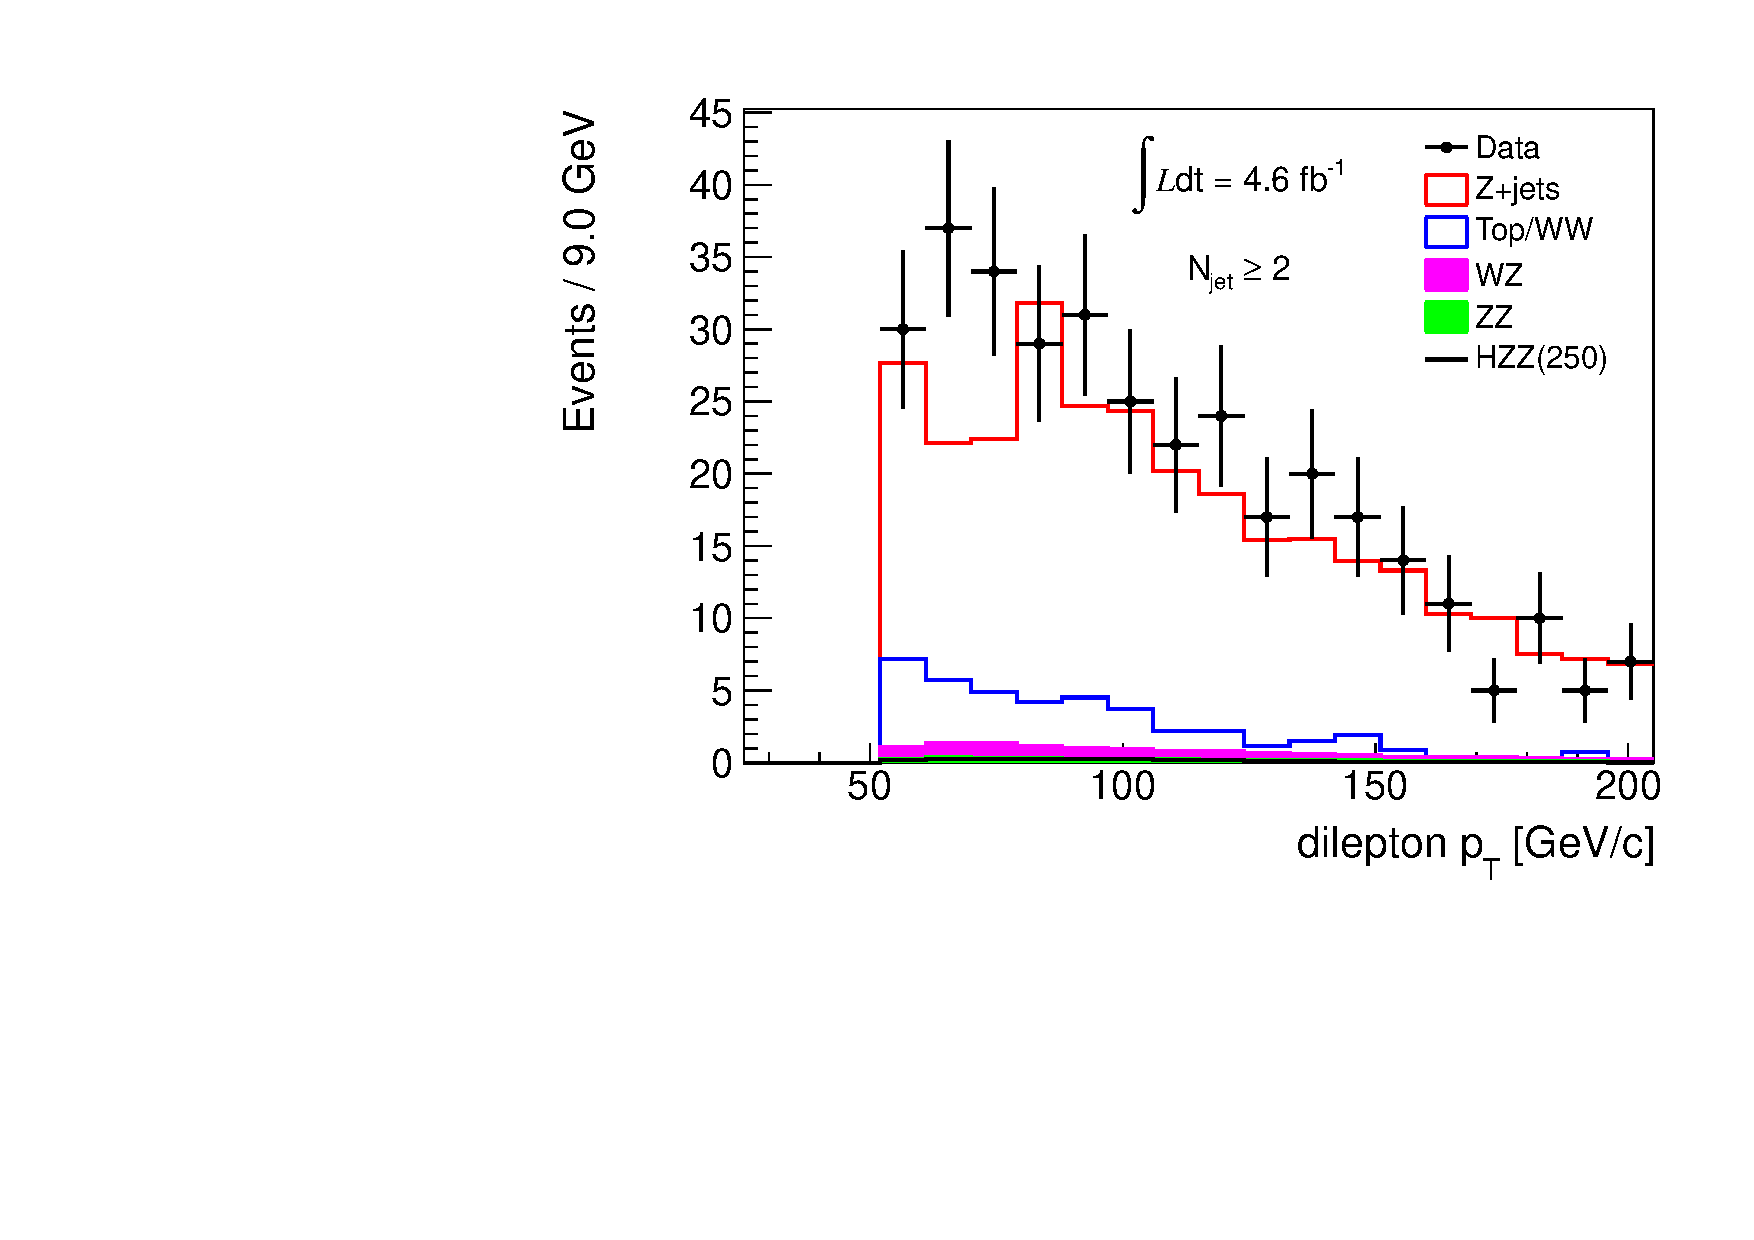
\includegraphics[width=.4\textwidth]{figures/presel_mH250_ee_dileppt_2j.pdf}}
\caption{Dilepton $p_T$ distribution in the electron channel after the $\ZZ$ preselection observed in data corresponding to $2.1$~\ifb data in 
the Inclusive~\subref{subfig:zpt_ee_incl}, 0-Jet~\subref{subfig:zpt_ee_0j}, 1-Jet~\subref{subfig:zpt_ee_1j} and 2-Jet~\subref{subfig:zpt_ee_2j} bins, 
compared to the expected from simulation for signal and background. The MC backgrounds are scaled as appropriate and the photon+jets estimate of the 
Z+jets background is added to the stack.}
\label{fig:zpt_zzpresel_ee}
\end{center}
\end{figure}
%%%%%%%%

%%%%%%%%
\begin{figure}[!hbtp]
\begin{center}
\subfigure[Inclusive]{\label{subfig:met_mm_incl}
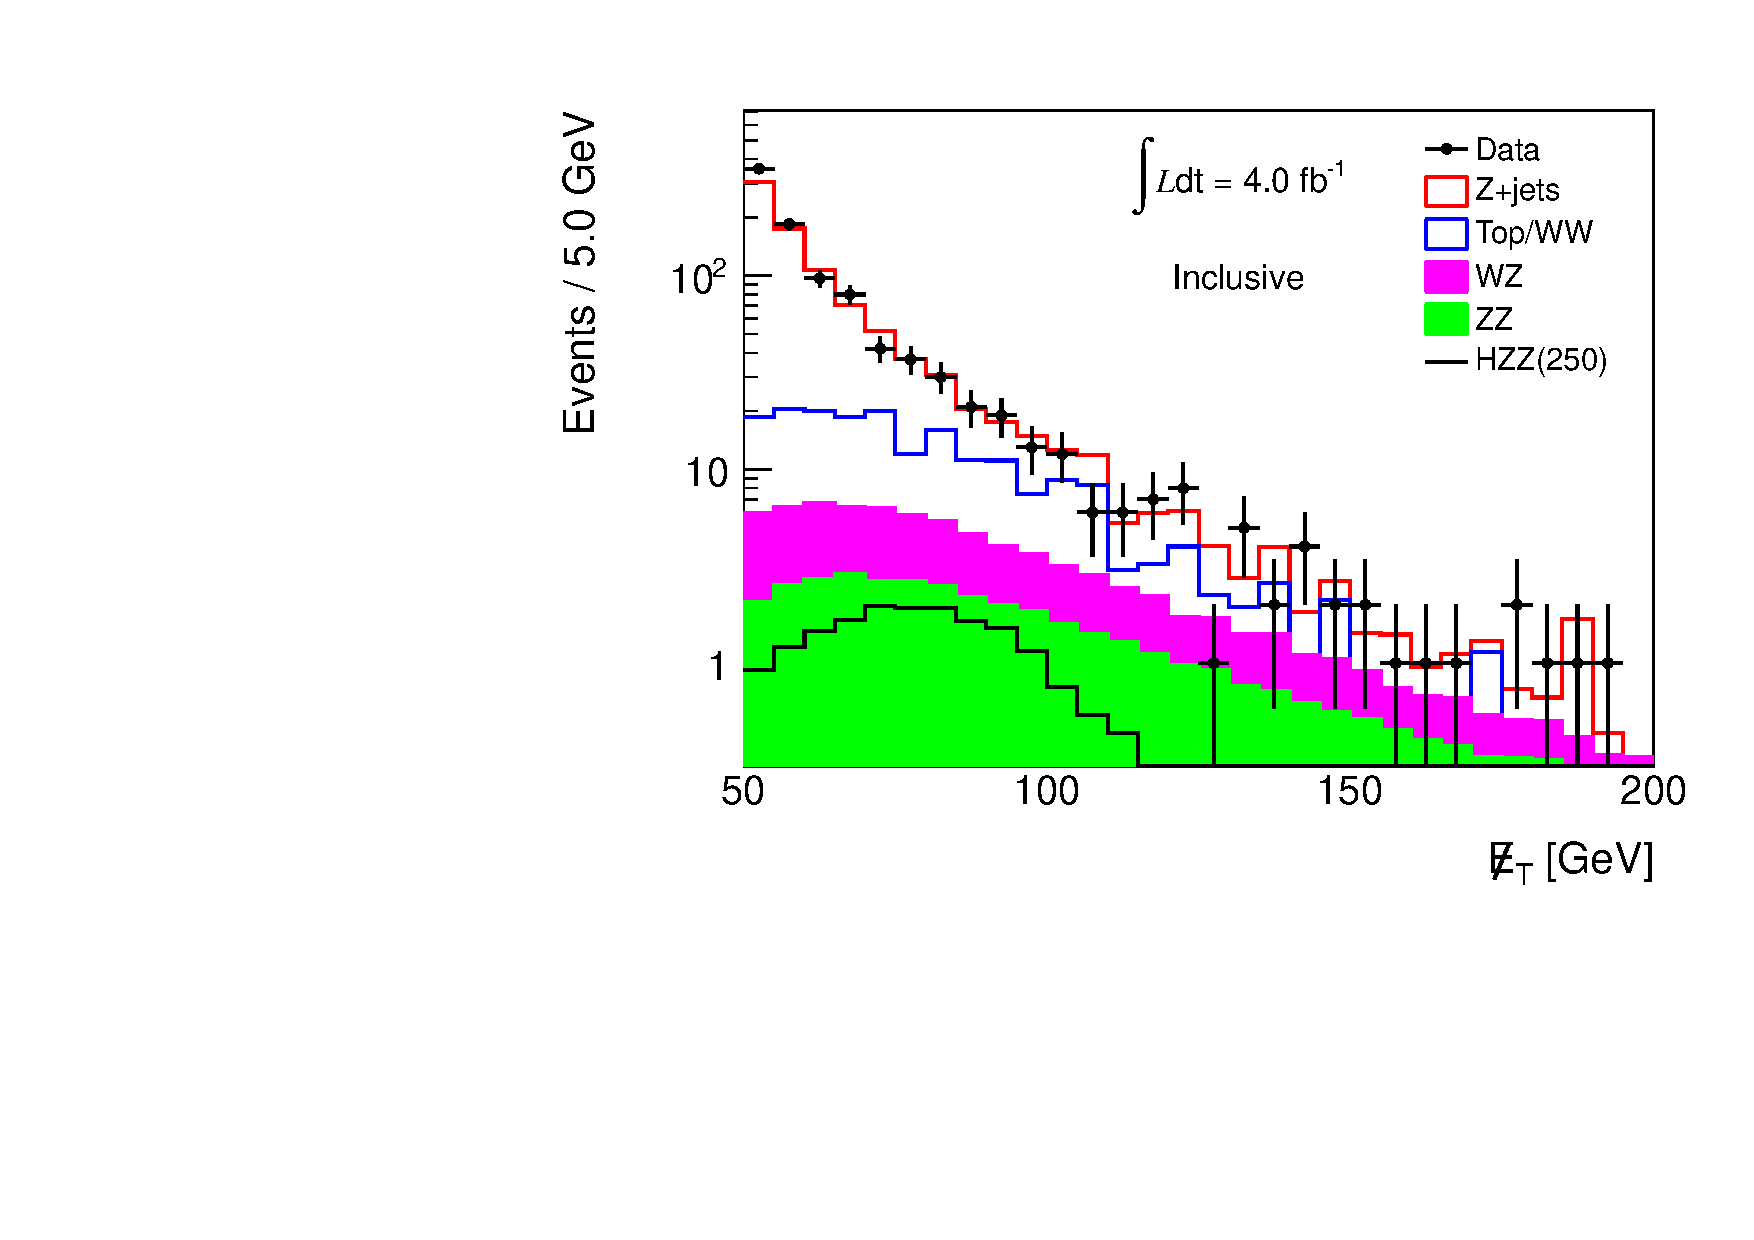
\includegraphics[width=.4\textwidth]{figures/presel_mH250_mm_metlog_incl.pdf}}
\subfigure[0-Jet]{\label{subfig:met_mm_0j}
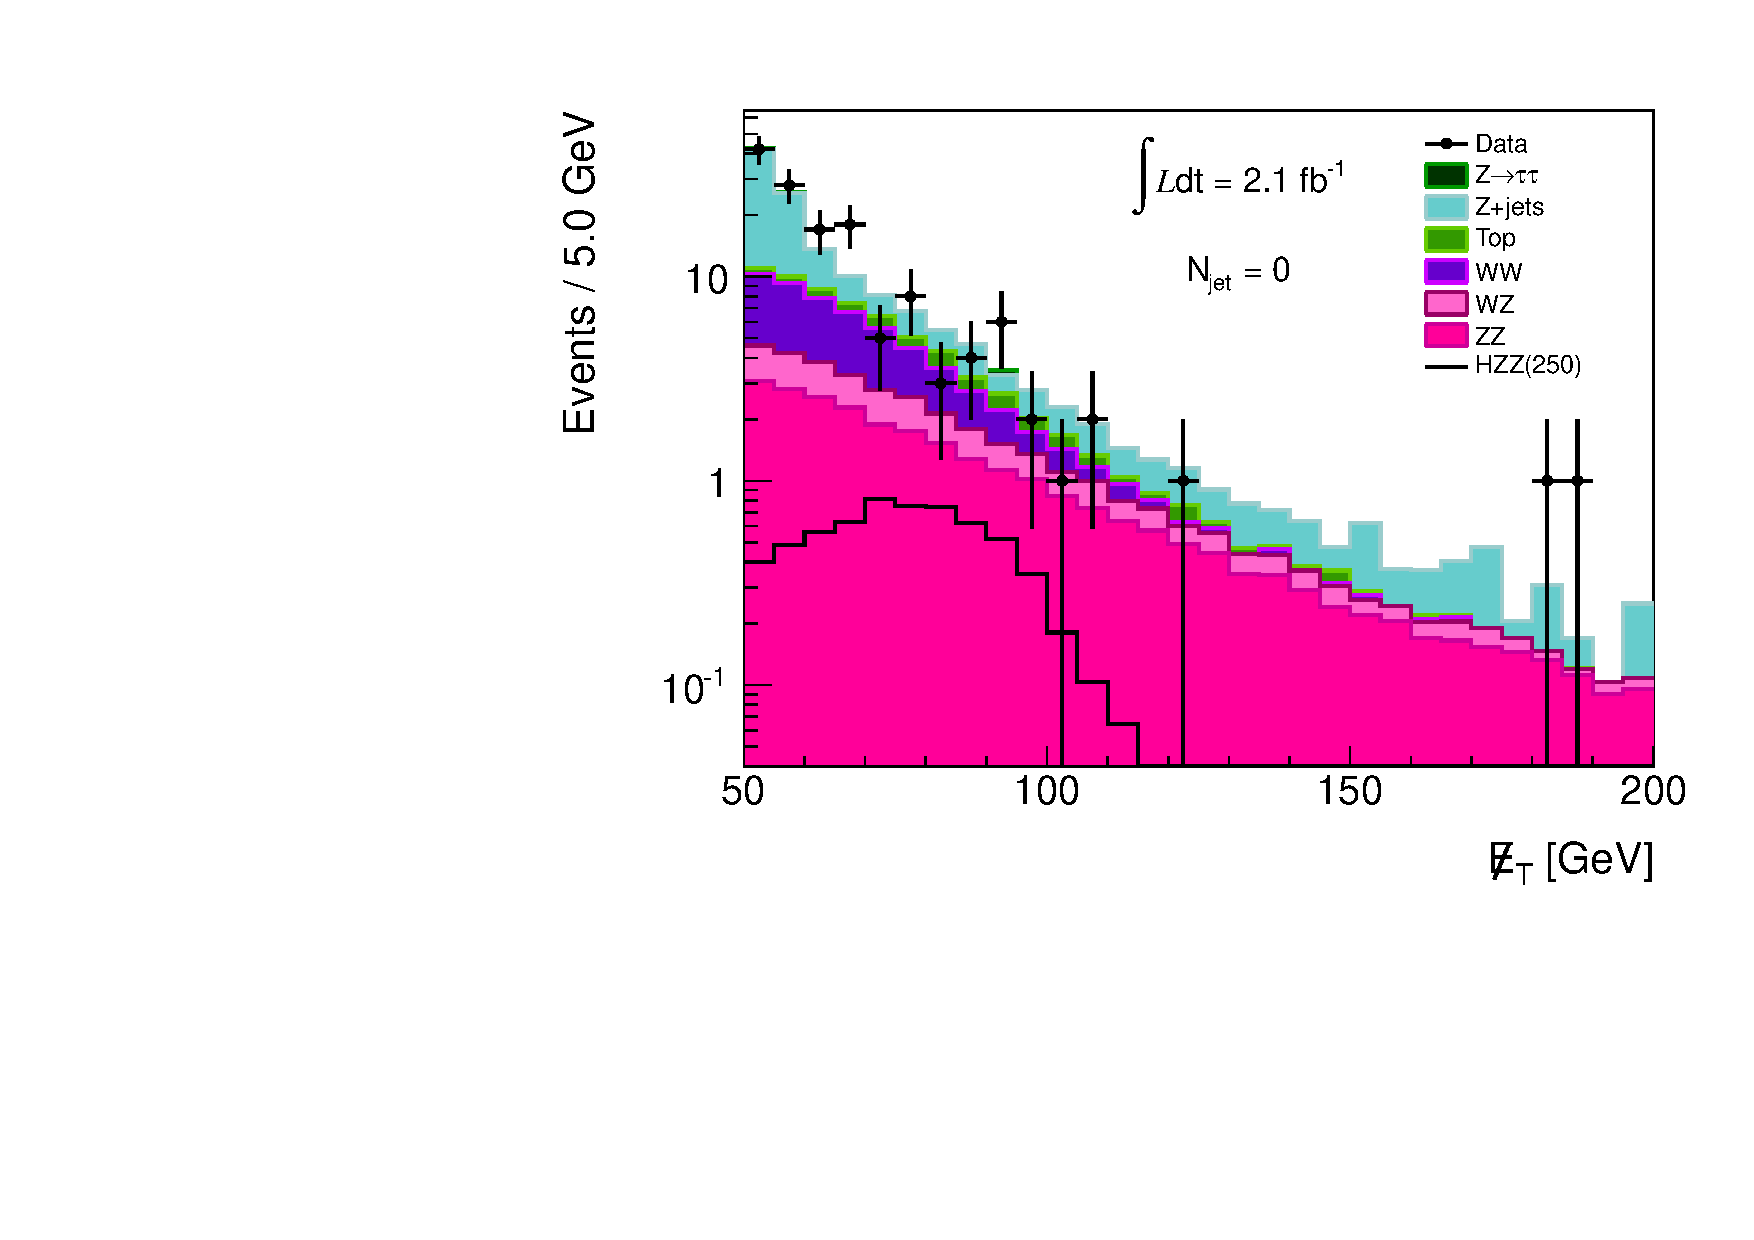
\includegraphics[width=.4\textwidth]{figures/presel_mH250_mm_metlog_0j.pdf}} \\
\subfigure[1-Jet]{\label{subfig:met_mm_1j}
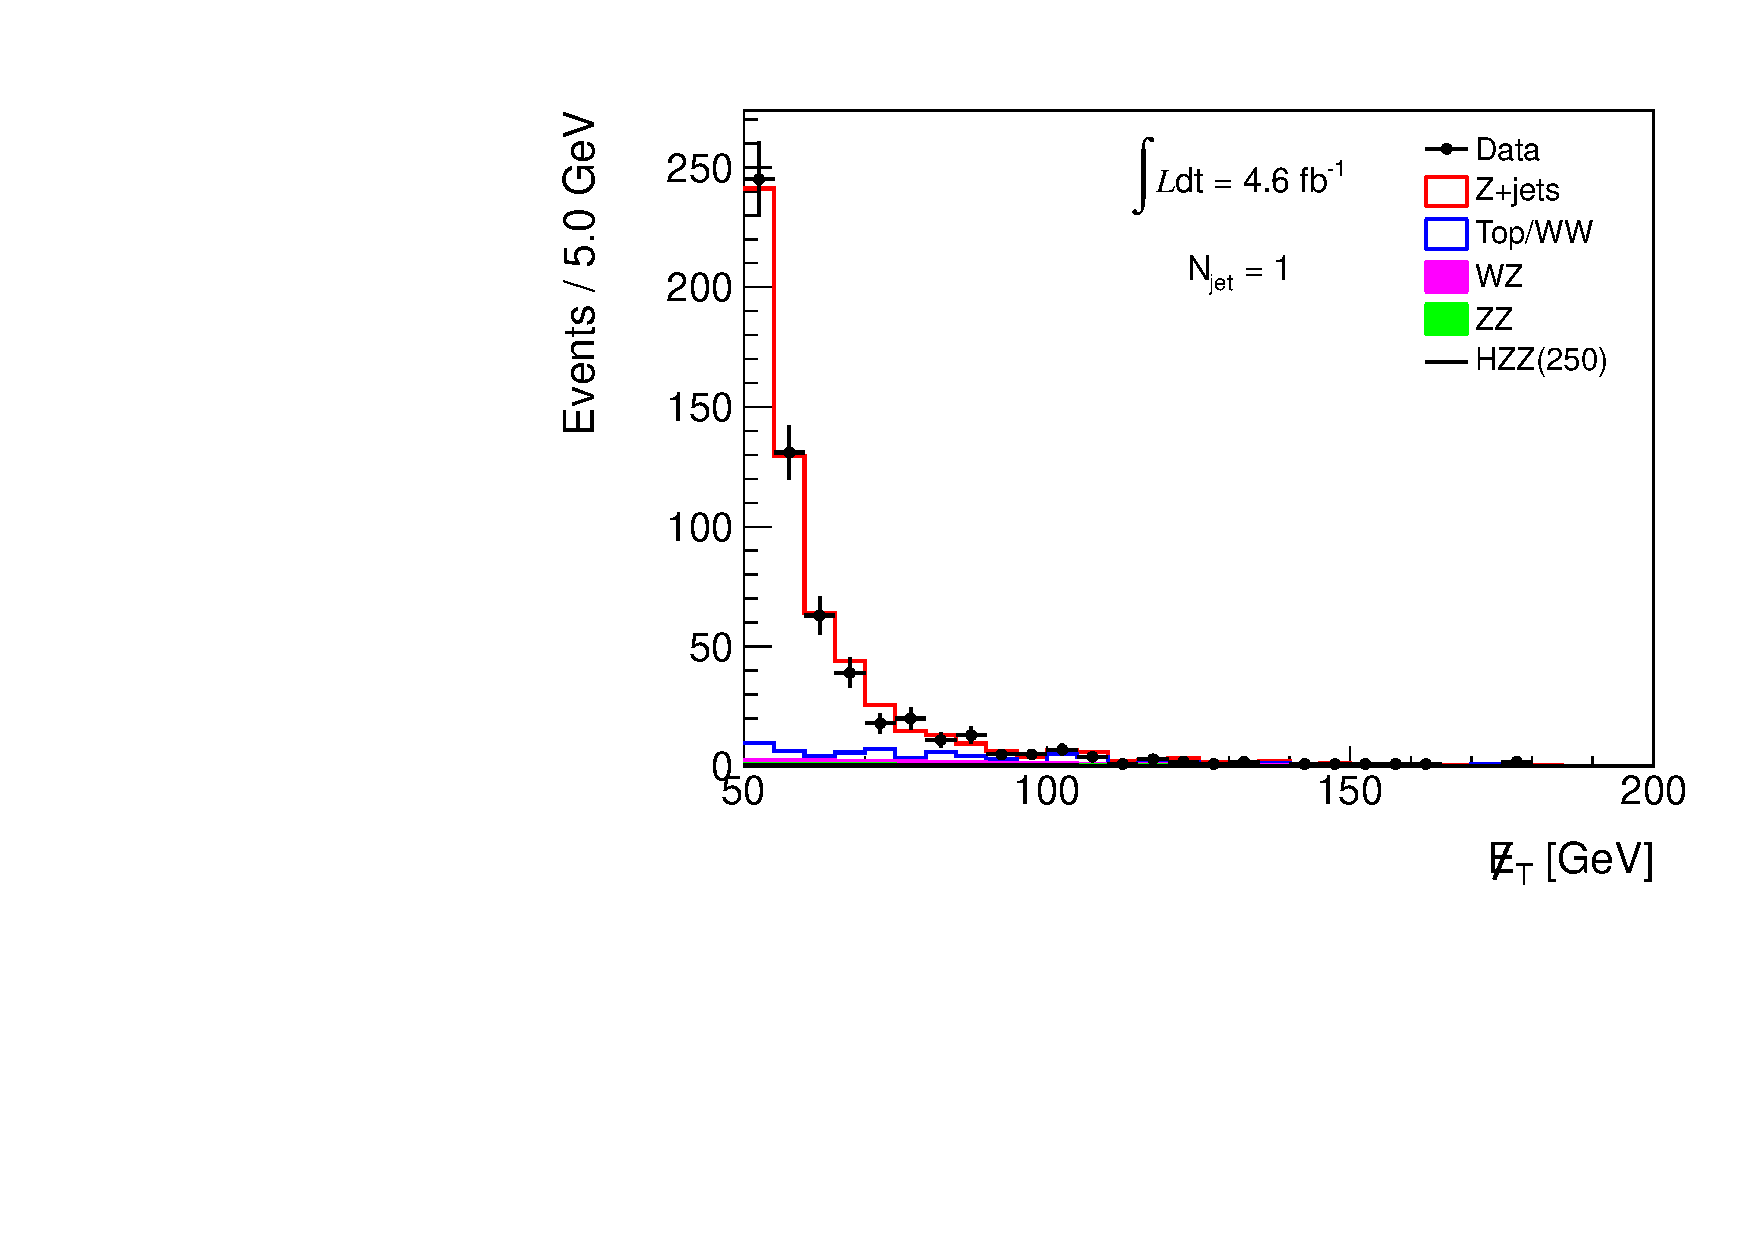
\includegraphics[width=.4\textwidth]{figures/presel_mH250_mm_metlog_1j.pdf}}
\subfigure[$\geq$2 Jets]{\label{subfig:met_mm_2j}
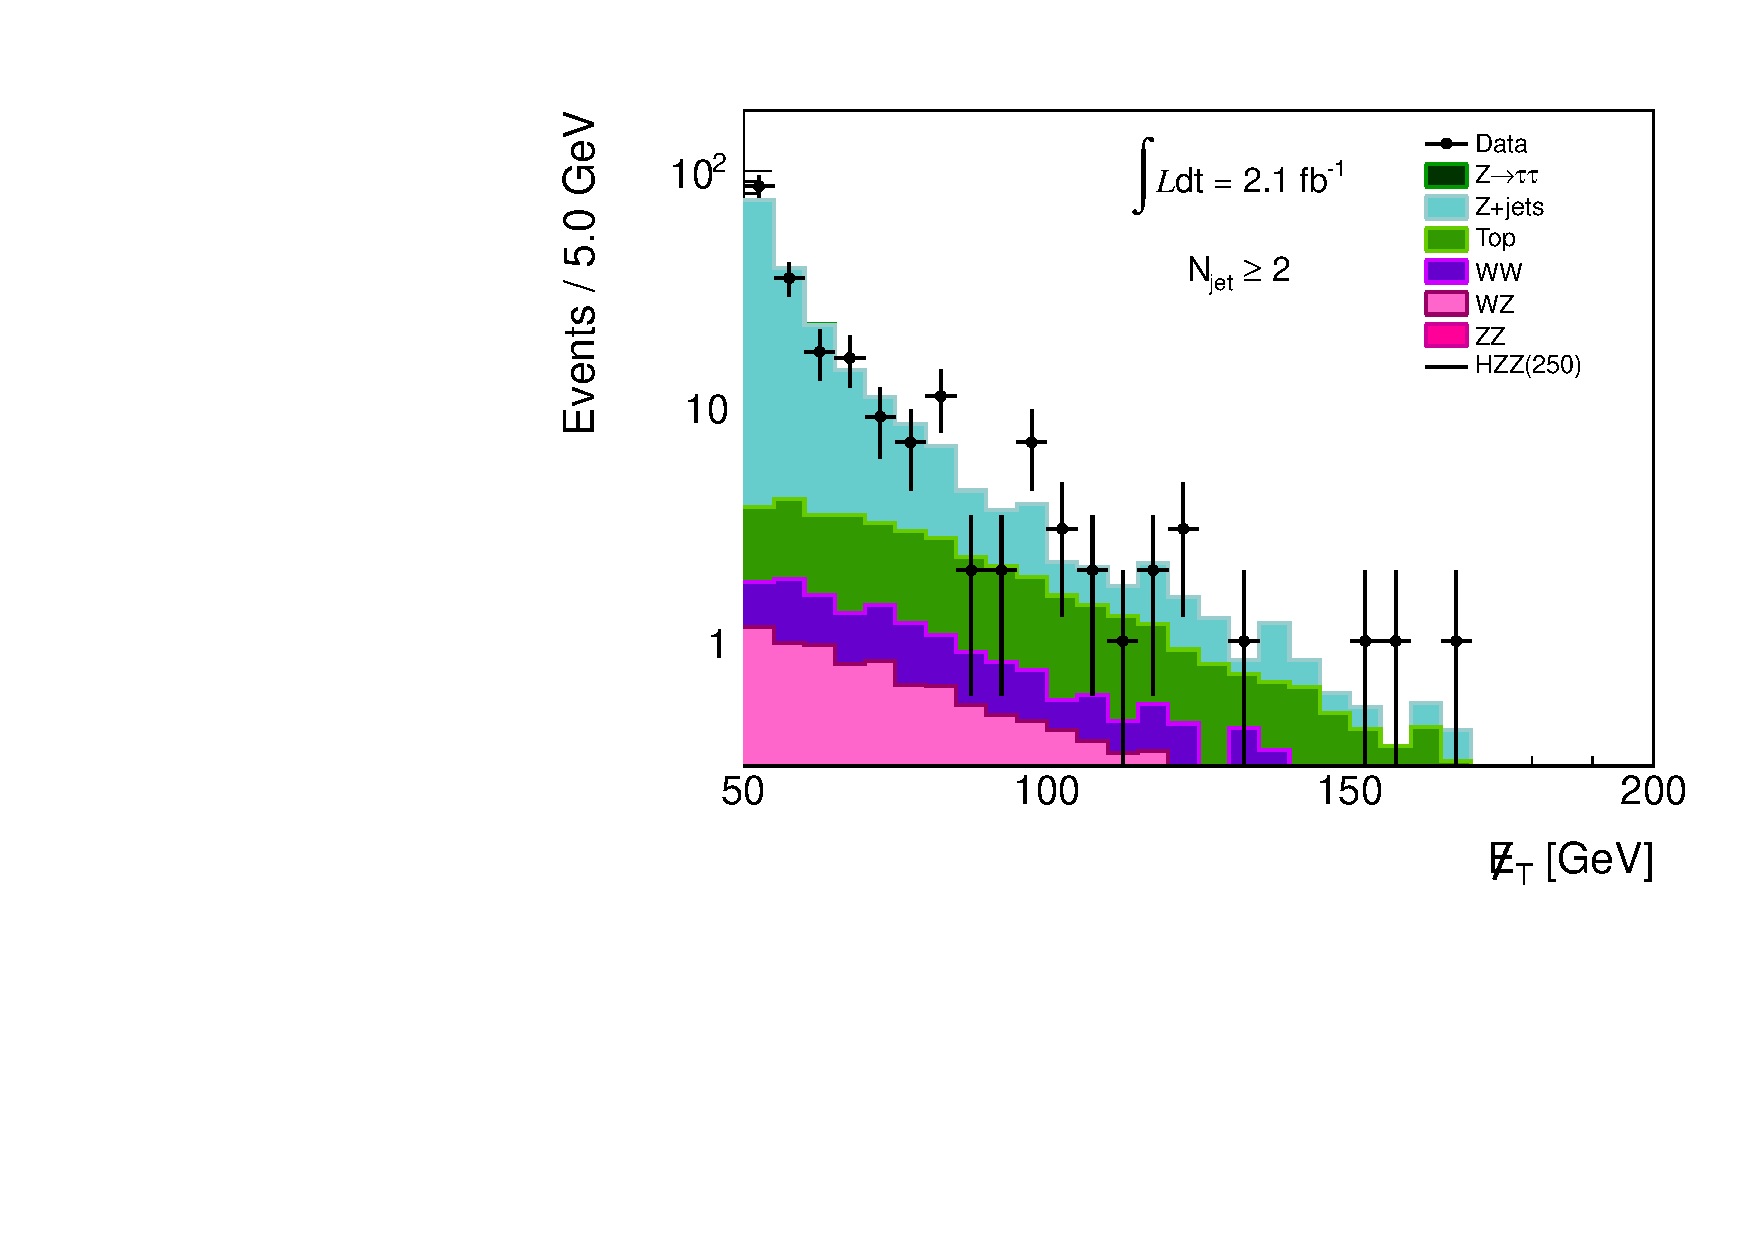
\includegraphics[width=.4\textwidth]{figures/presel_mH250_mm_metlog_2j.pdf}}
\caption{Missing transverse energy distribution in the muon channel after the $\ZZ$ preselection observed in data corresponding to $2.1$~\ifb data in 
the Inclusive~\subref{subfig:met_mm_incl}, 0-Jet~\subref{subfig:met_mm_0j}, 1-Jet~\subref{subfig:met_mm_1j} and 2-Jet~\subref{subfig:met_mm_2j} bins, 
compared to the expected from simulation for signal and background. The MC backgrounds are scaled as appropriate and the photon+jets estimate of the 
Z+jets background is added to the stack.}
\label{fig:met_zzpresel_mm}
\end{center}
\end{figure}
%%%%%%%%

%%%%%%%%
\begin{figure}[!hbtp]
\begin{center}
\subfigure[Inclusive]{\label{subfig:met_ee_incl}
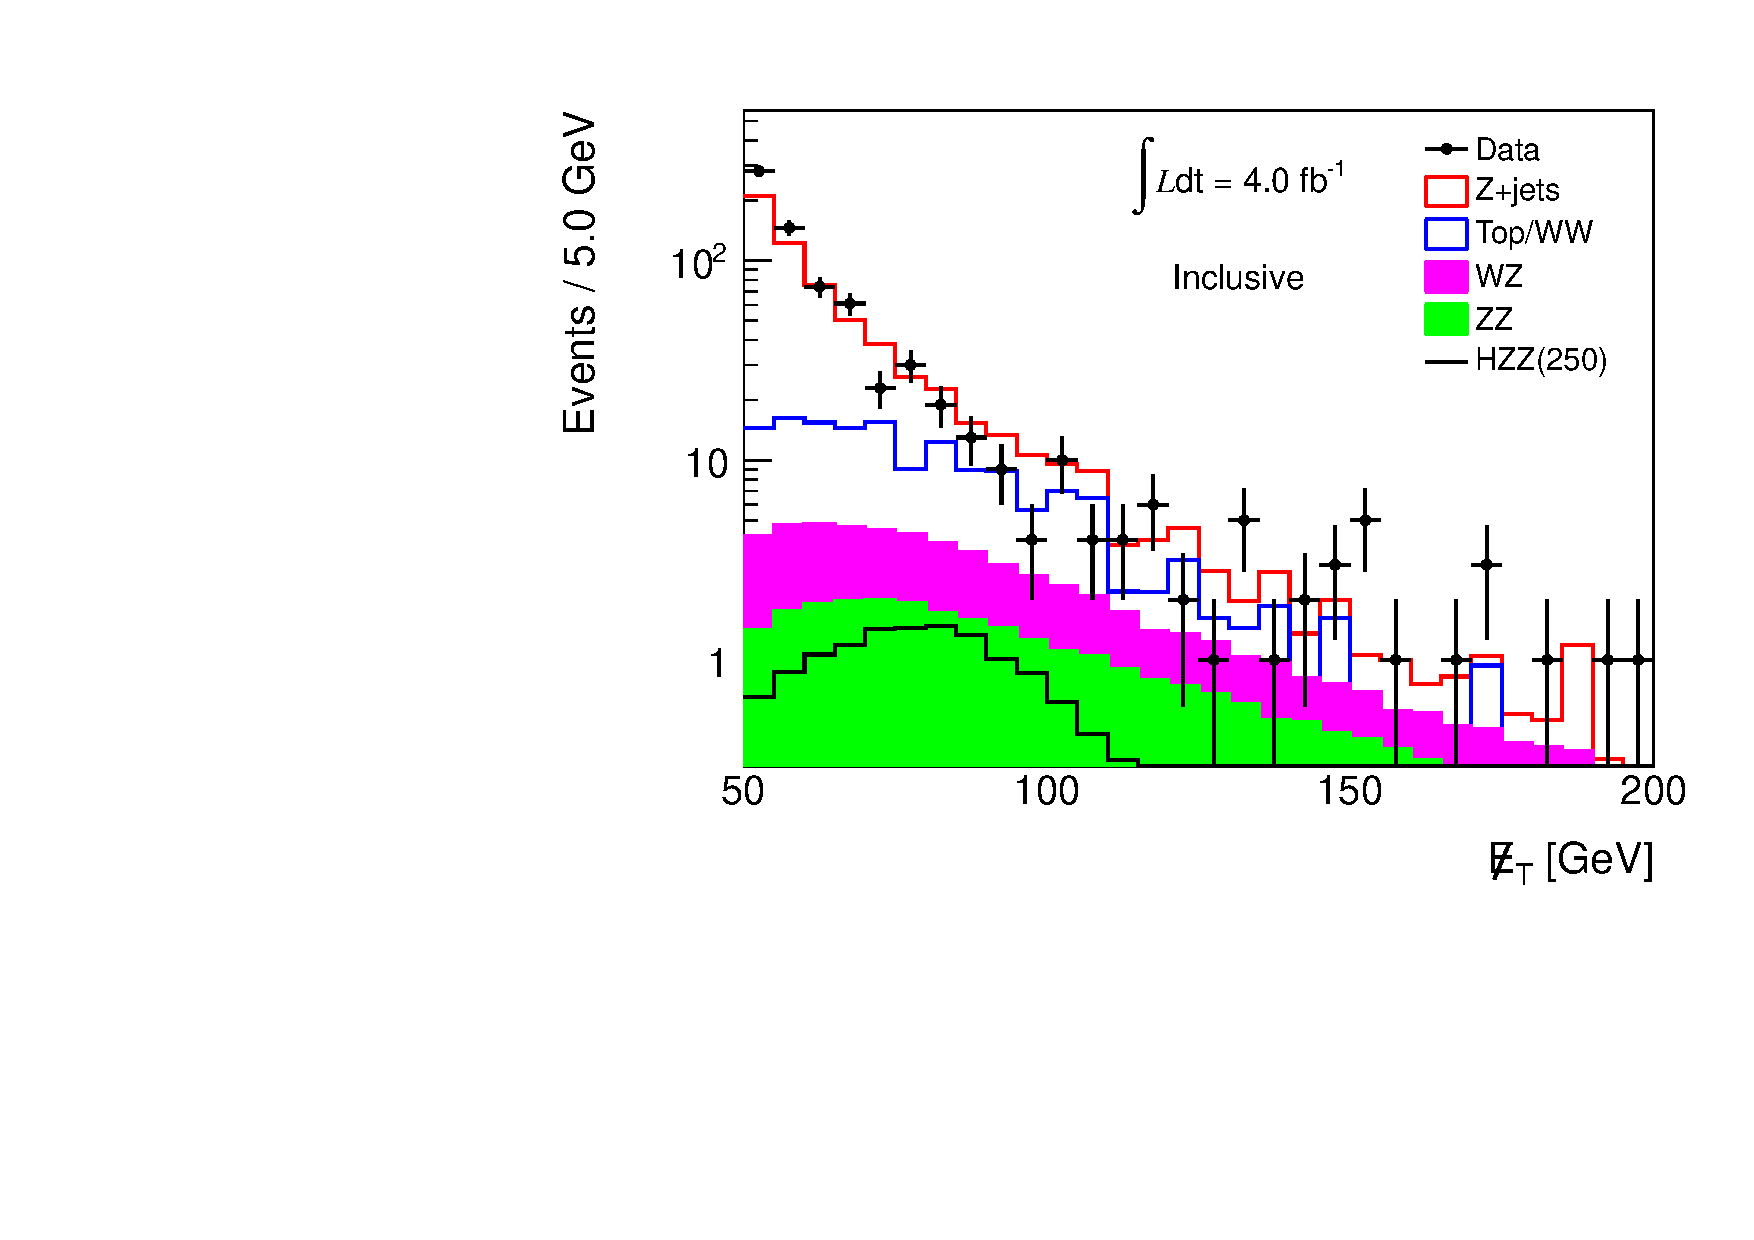
\includegraphics[width=.4\textwidth]{figures/presel_mH250_ee_metlog_incl.pdf}}
\subfigure[0-Jet]{\label{subfig:met_ee_0j}
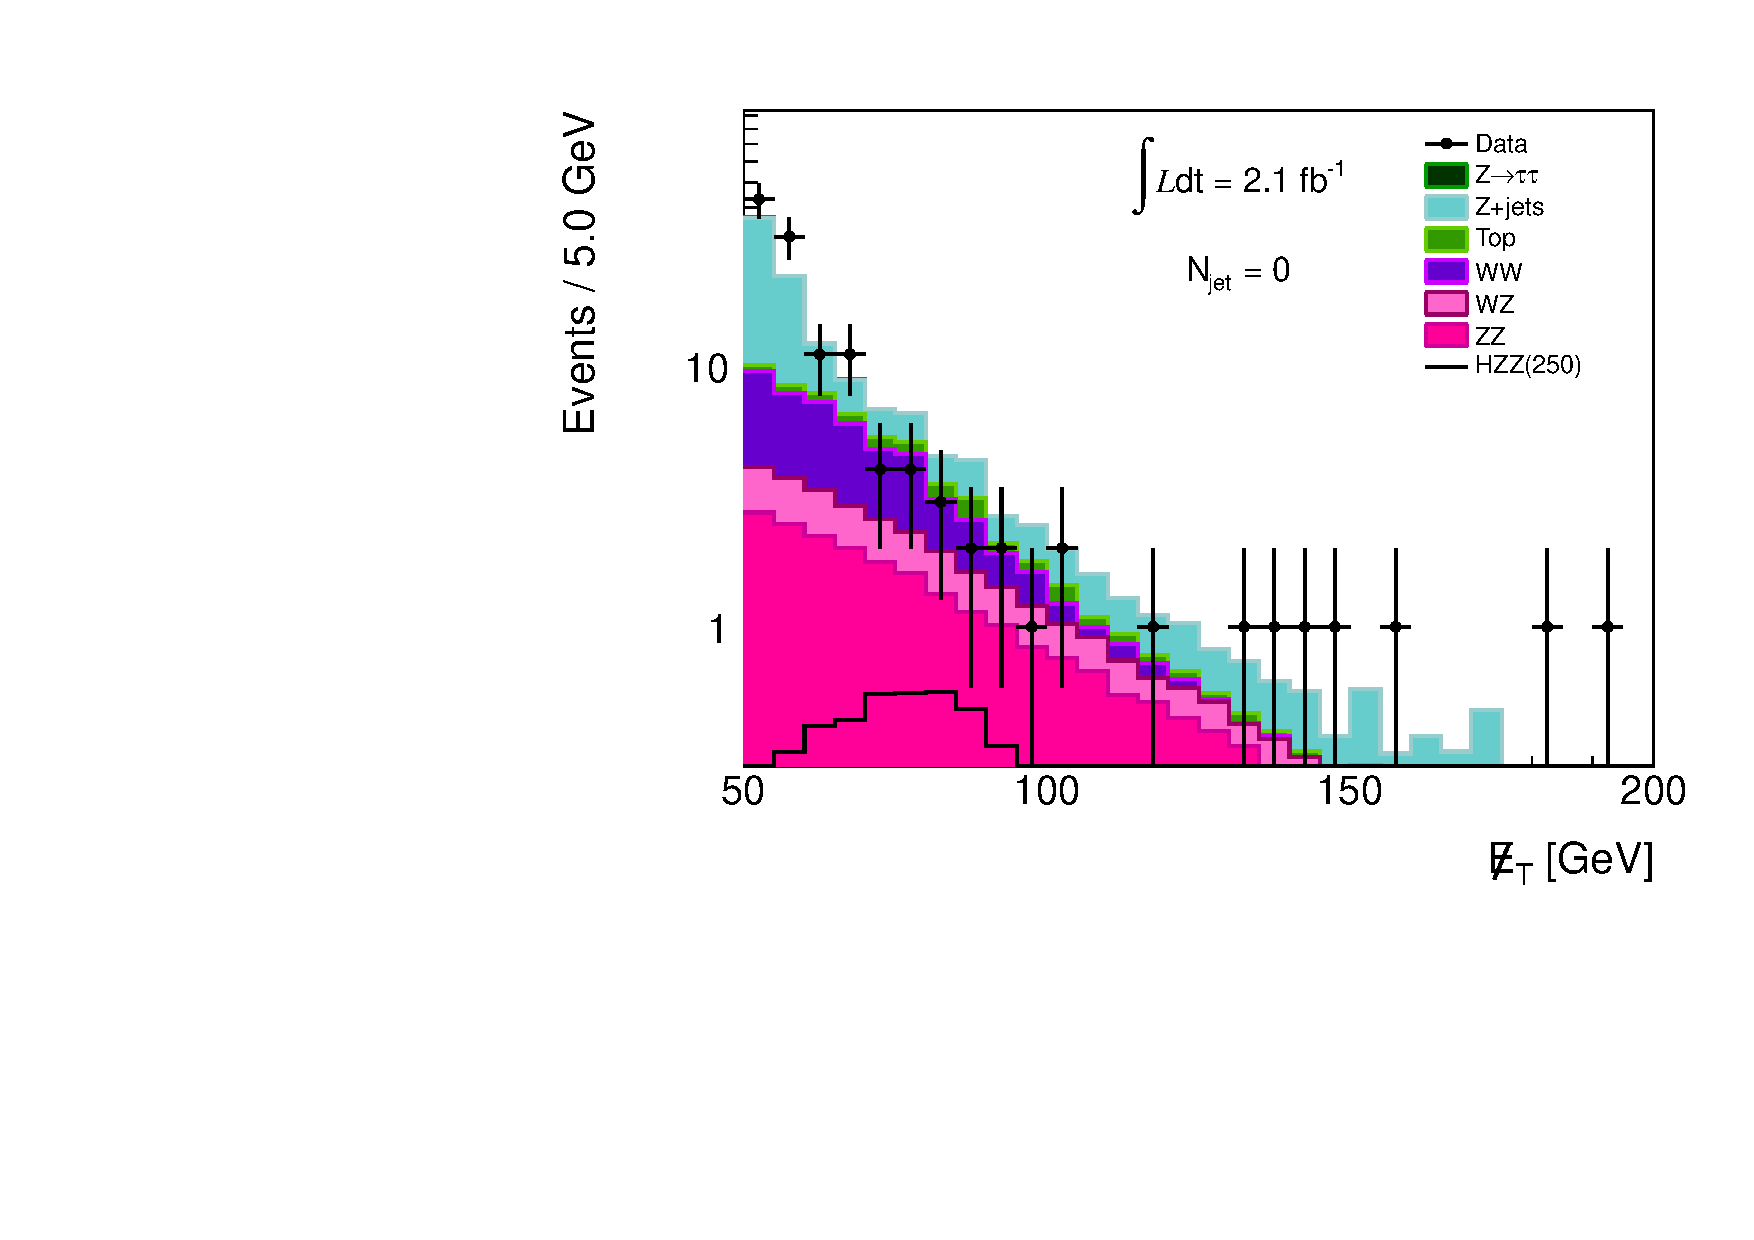
\includegraphics[width=.4\textwidth]{figures/presel_mH250_ee_metlog_0j.pdf}} \\
\subfigure[1-Jet]{\label{subfig:met_ee_1j}
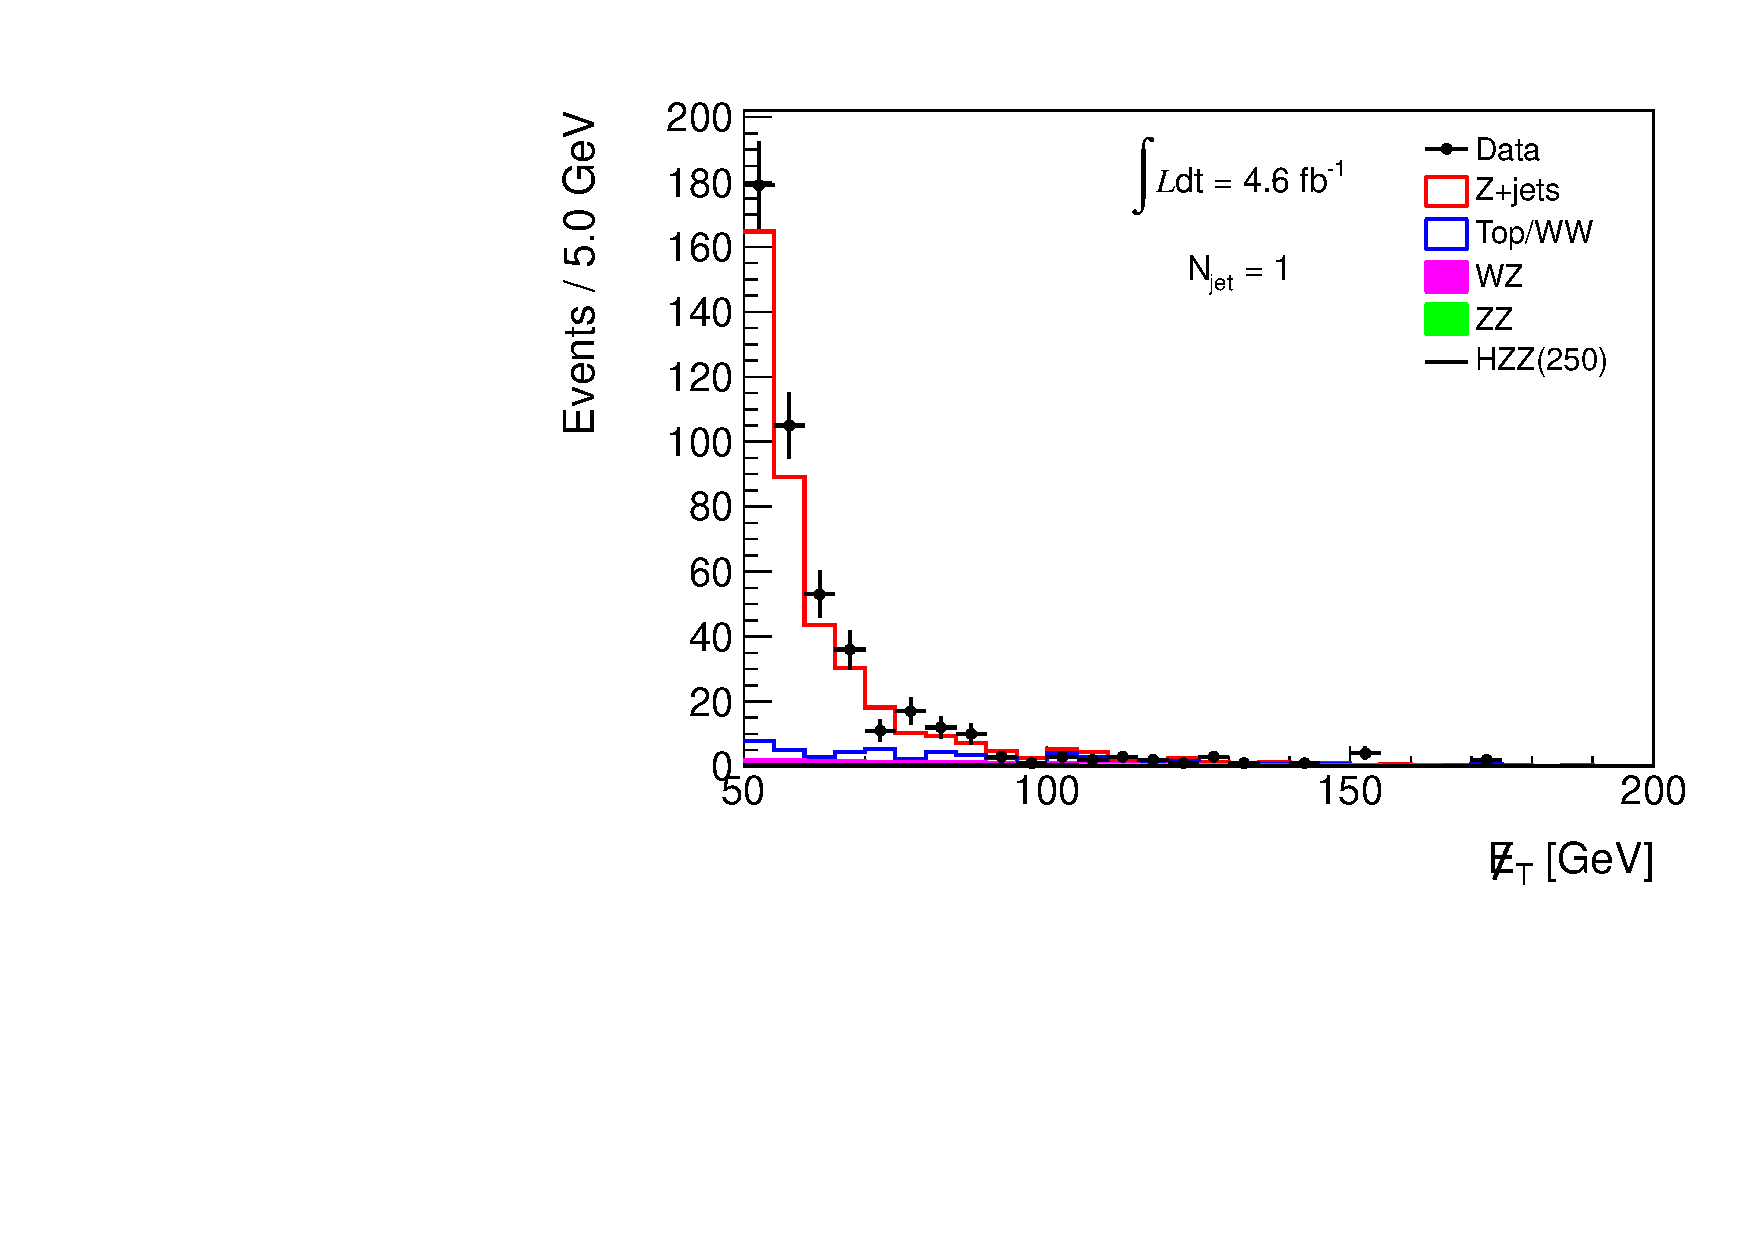
\includegraphics[width=.4\textwidth]{figures/presel_mH250_ee_metlog_1j.pdf}}
\subfigure[$\geq$2 Jets]{\label{subfig:met_ee_2j}
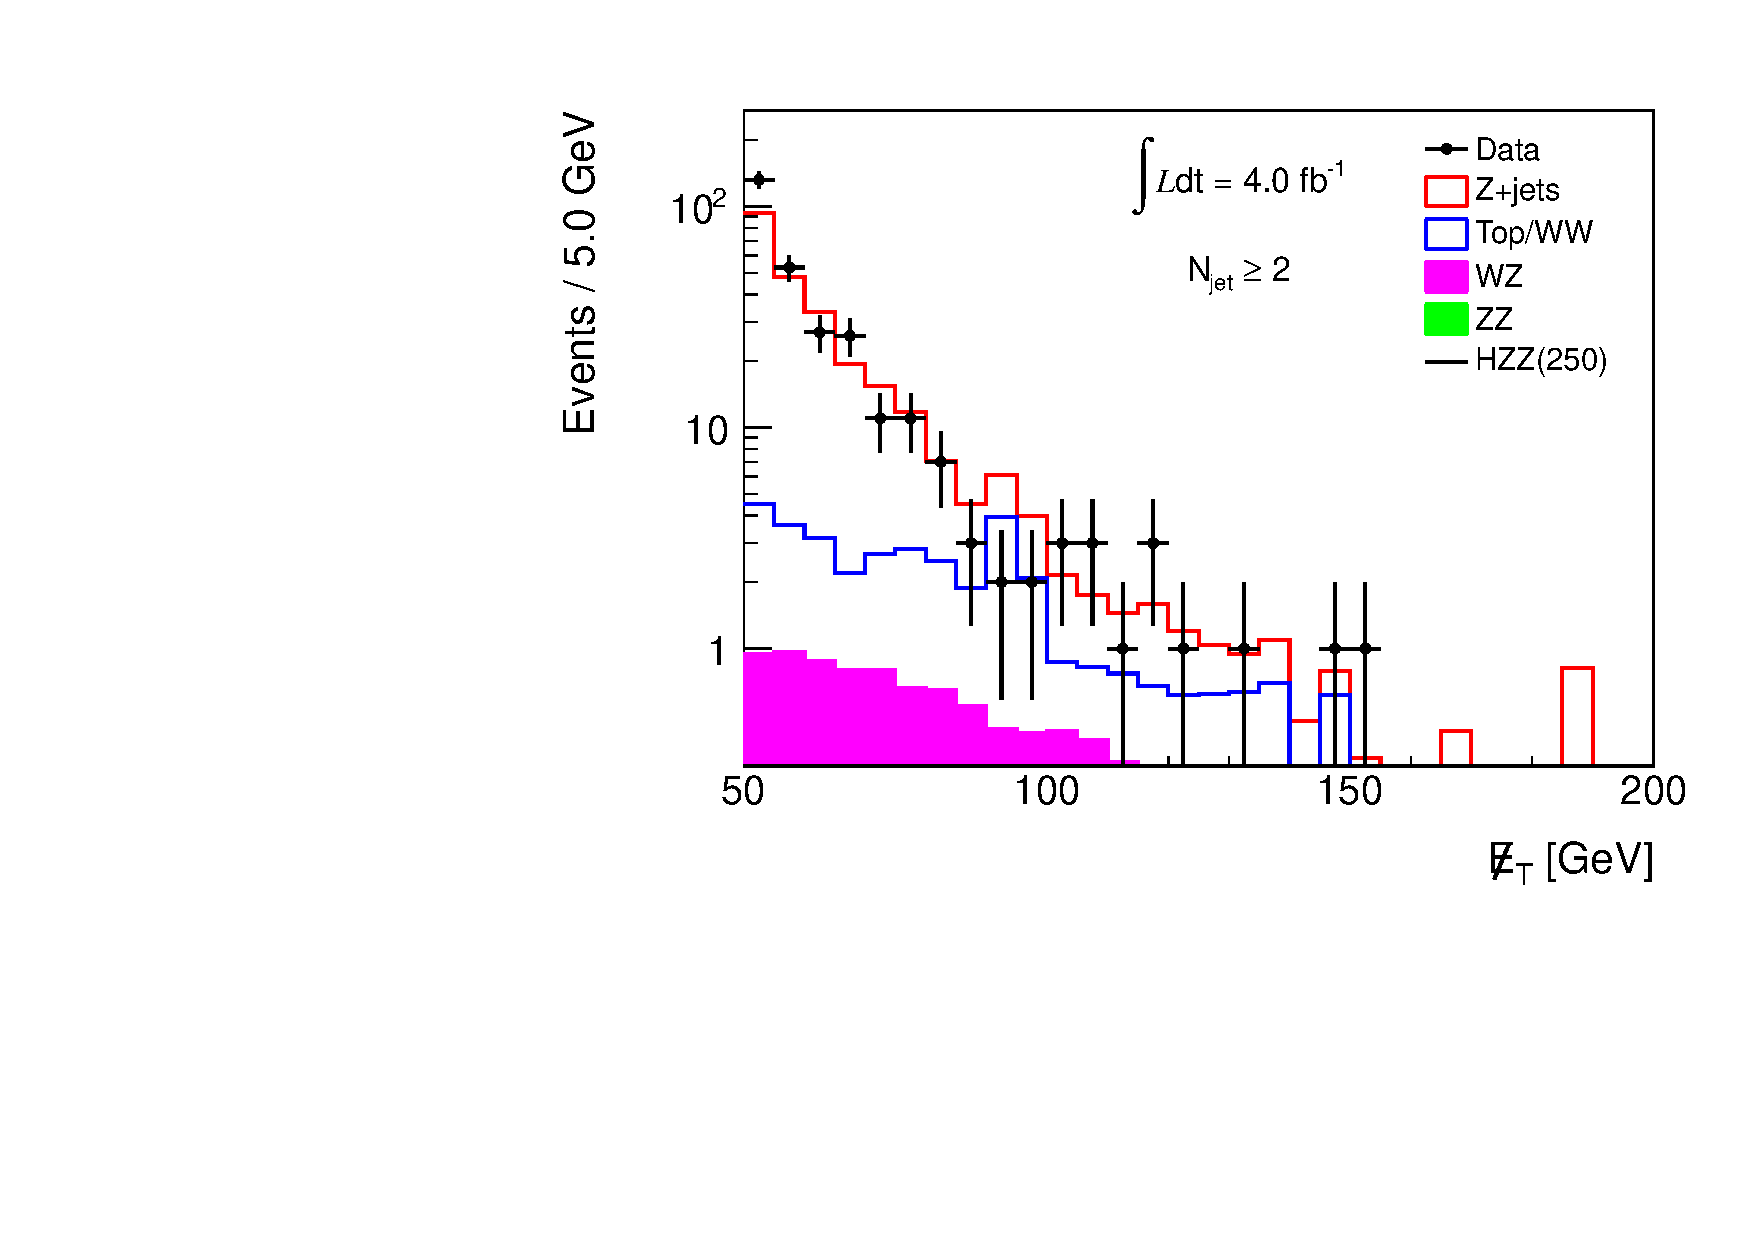
\includegraphics[width=.4\textwidth]{figures/presel_mH250_ee_metlog_2j.pdf}}
\caption{Missing transverse energy distribution in the electron channel after the $\ZZ$ preselection observed in data corresponding to $2.1$~\ifb data in 
the Inclusive~\subref{subfig:met_ee_incl}, 0-Jet~\subref{subfig:met_ee_0j}, 1-Jet~\subref{subfig:met_ee_1j} and 2-Jet~\subref{subfig:met_ee_2j} bins, 
compared to the expected from simulation for signal and background. The MC backgrounds are scaled as appropriate and the photon+jets estimate of the 
Z+jets background is added to the stack.}
\label{fig:met_zzpresel_ee}
\end{center}
\end{figure}
%%%%%%%%

%%%%%%%%
\begin{figure}[!hbtp]
\begin{center}
\subfigure[Inclusive]{\label{subfig:mt_mm_incl}
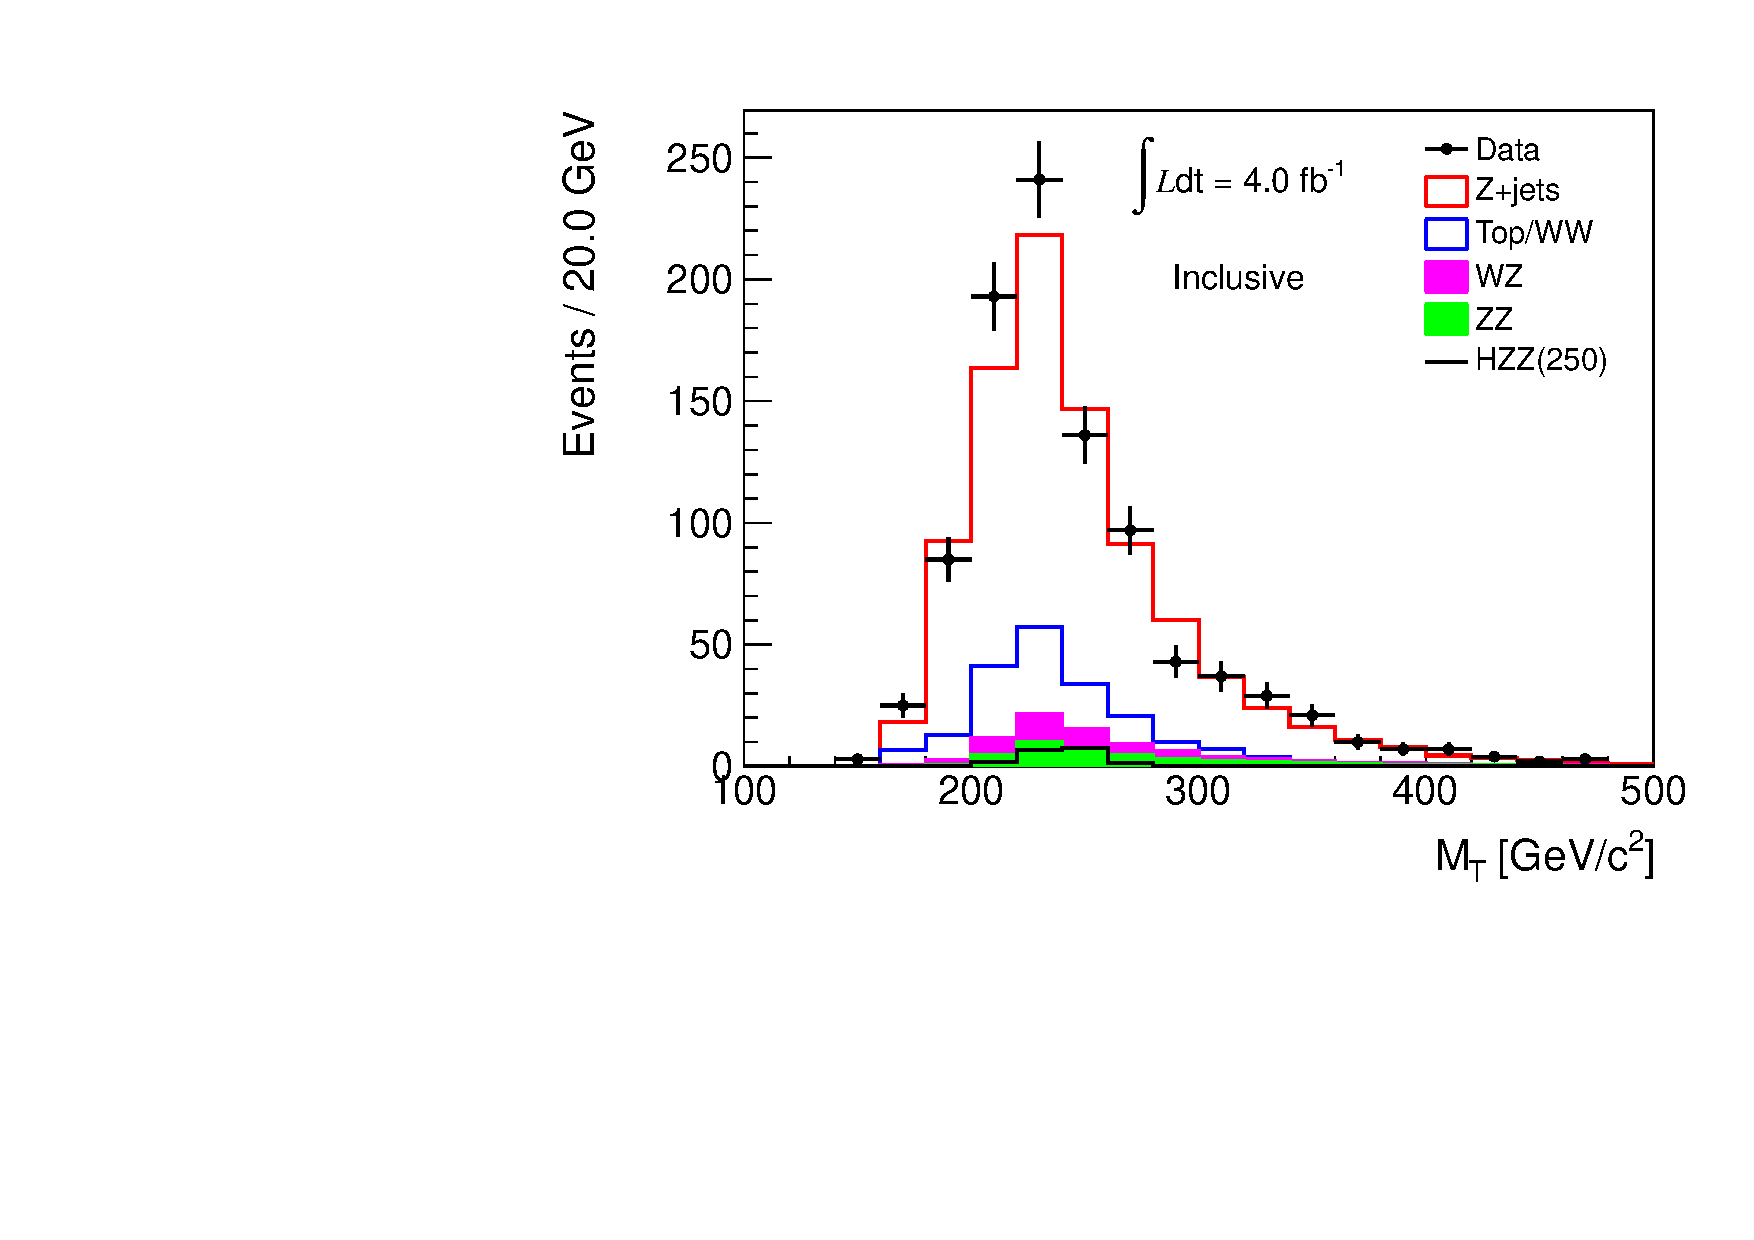
\includegraphics[width=.4\textwidth]{figures/presel_mH250_mm_mt_incl.pdf}}
\subfigure[0-Jet]{\label{subfig:mt_mm_0j}
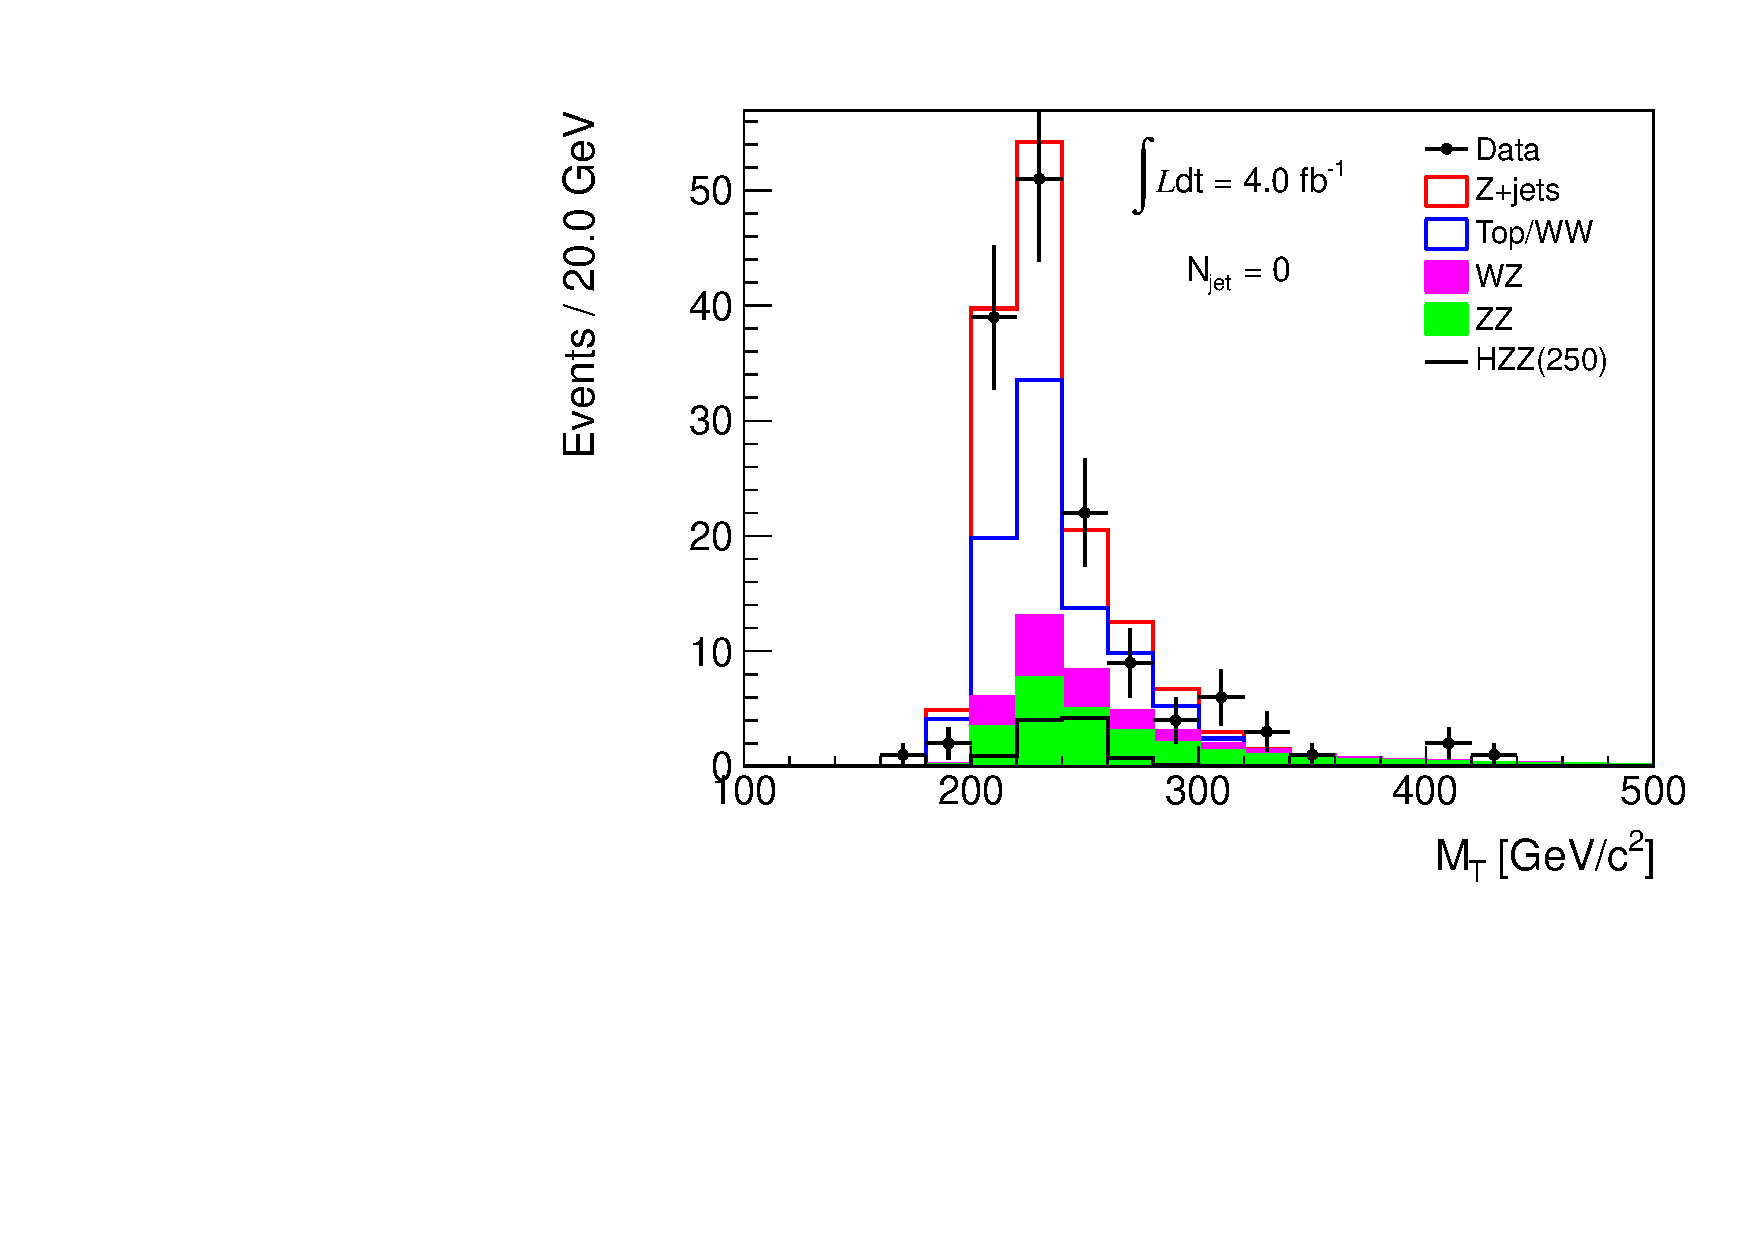
\includegraphics[width=.4\textwidth]{figures/presel_mH250_mm_mt_0j.pdf}} \\
\subfigure[1-Jet]{\label{subfig:mt_mm_1j}
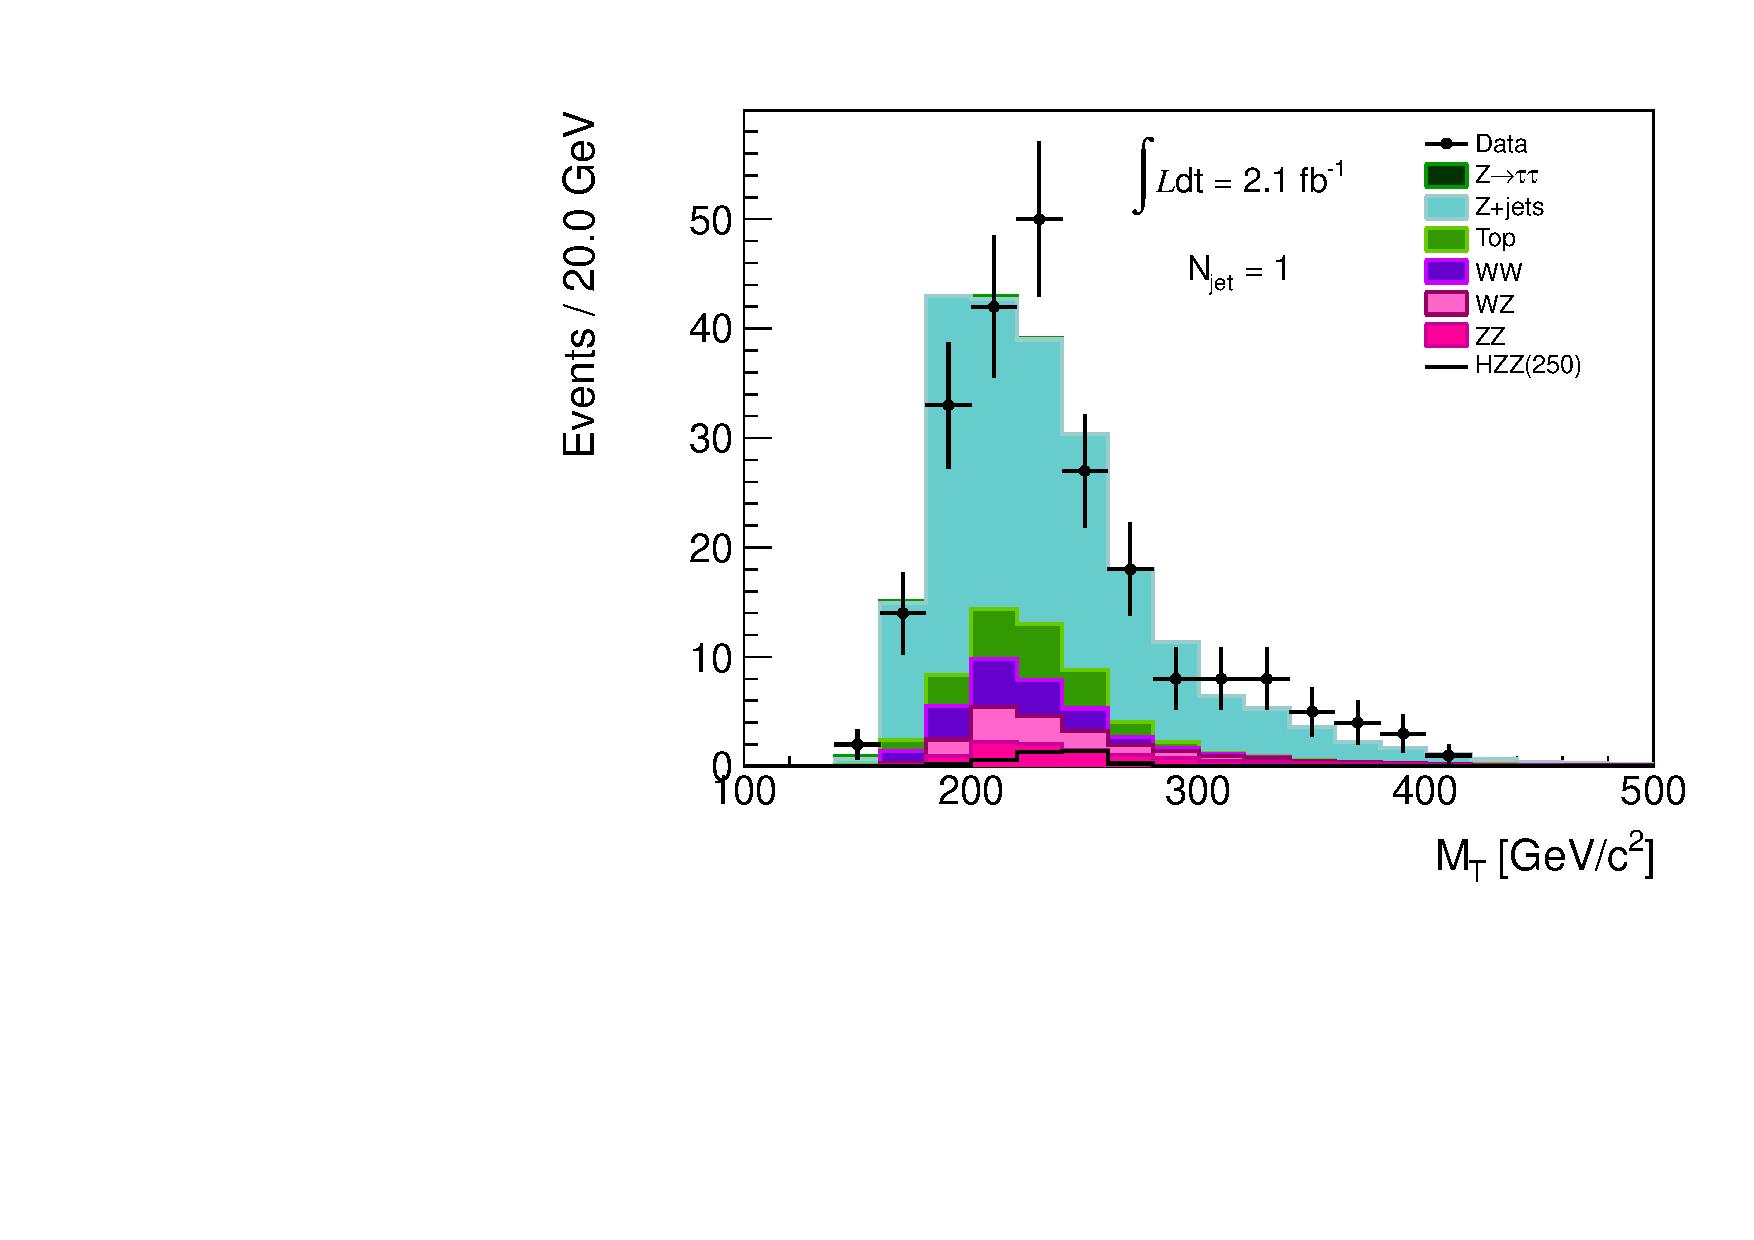
\includegraphics[width=.4\textwidth]{figures/presel_mH250_mm_mt_1j.pdf}}
\subfigure[$\geq$2 Jets]{\label{subfig:mt_mm_2j}
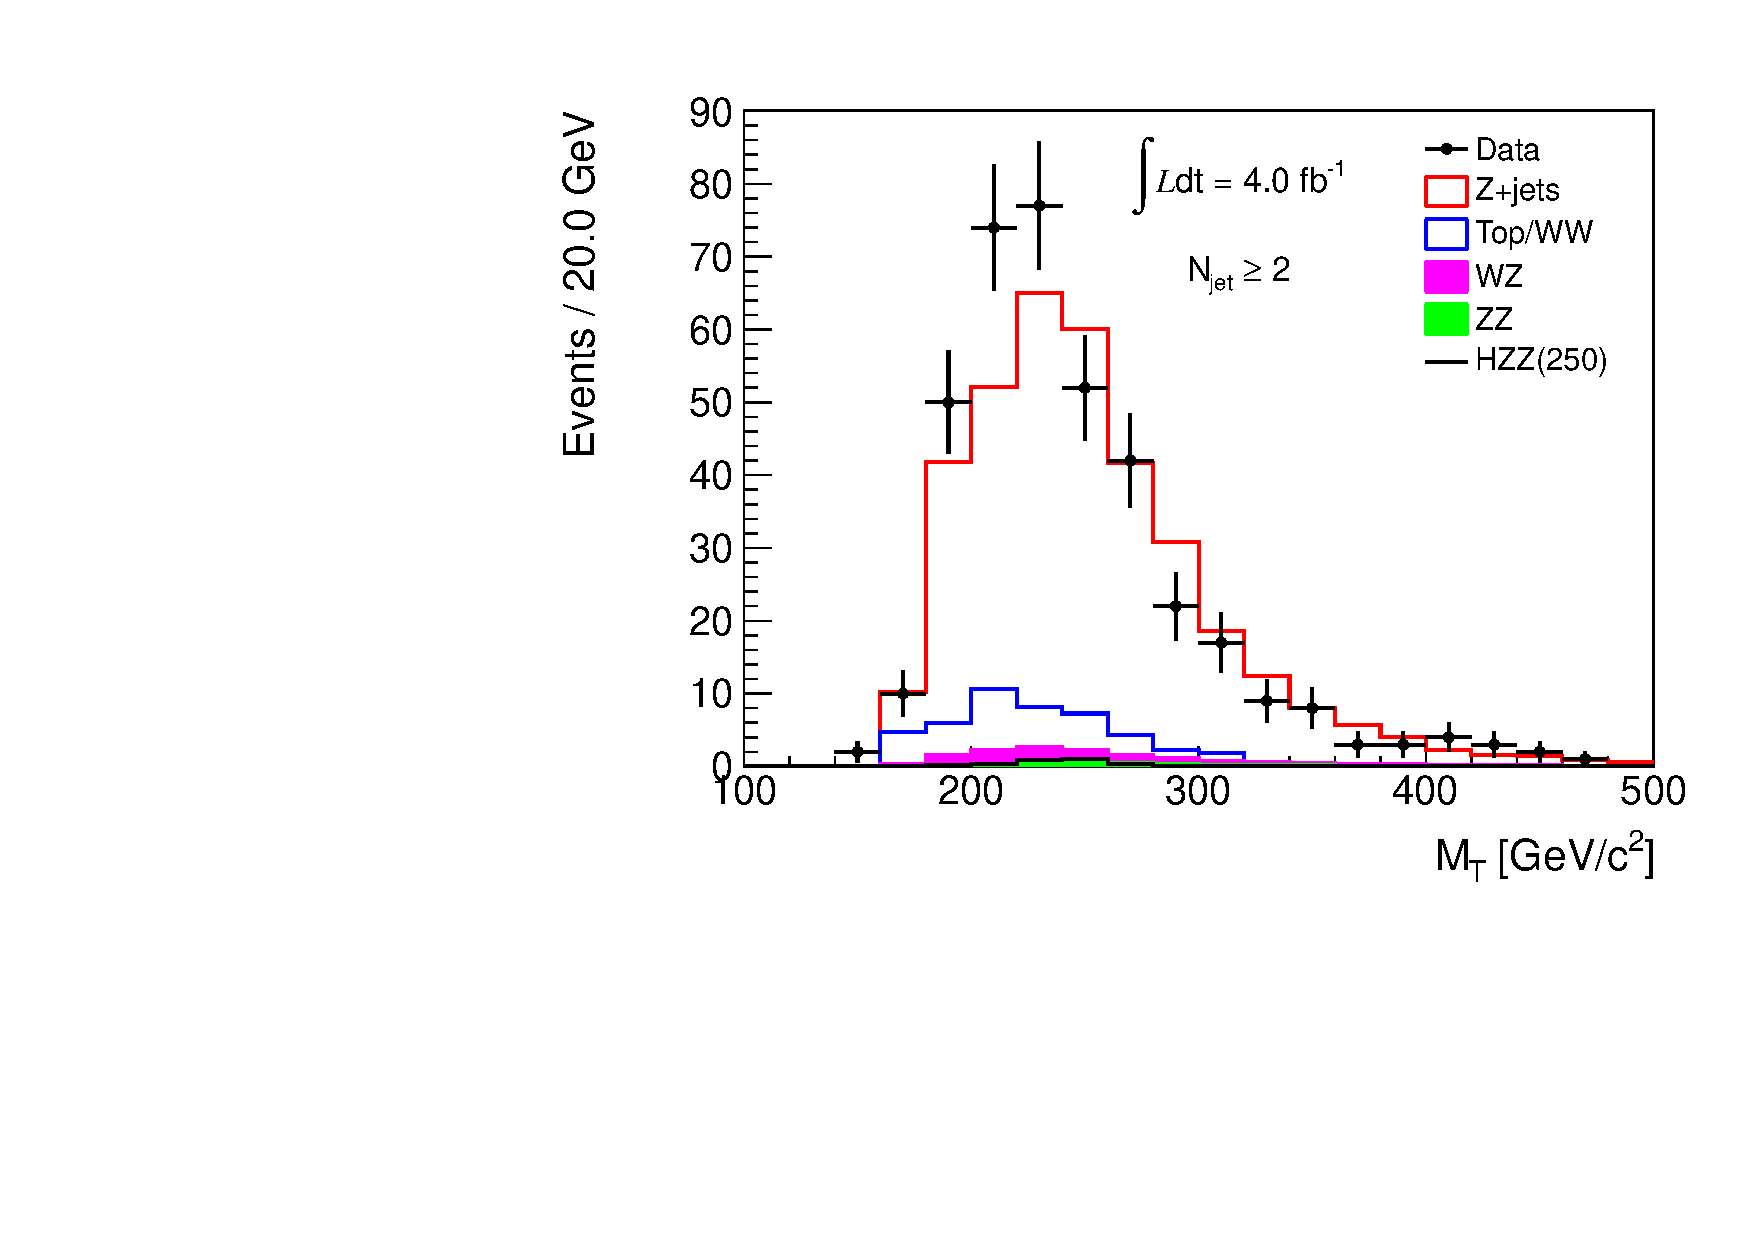
\includegraphics[width=.4\textwidth]{figures/presel_mH250_mm_mt_2j.pdf}}
\caption{Transverse mass distribution in the muon channel after the $\ZZ$ preselection observed in data corresponding to $2.1$~\ifb data in 
the Inclusive~\subref{subfig:mt_mm_incl}, 0-Jet~\subref{subfig:mt_mm_0j}, 1-Jet~\subref{subfig:mt_mm_1j} and 2-Jet~\subref{subfig:mt_mm_2j} bins, 
compared to the expected from simulation for signal and background. The MC backgrounds are scaled as appropriate and the photon+jets estimate of the 
Z+jets background is added to the stack.}
\label{fig:mt_zzpresel_mm}
\end{center}
\end{figure}
%%%%%%%%

%%%%%%%%
\begin{figure}[!hbtp]
\begin{center}
\subfigure[Inclusive]{\label{subfig:mt_ee_incl}
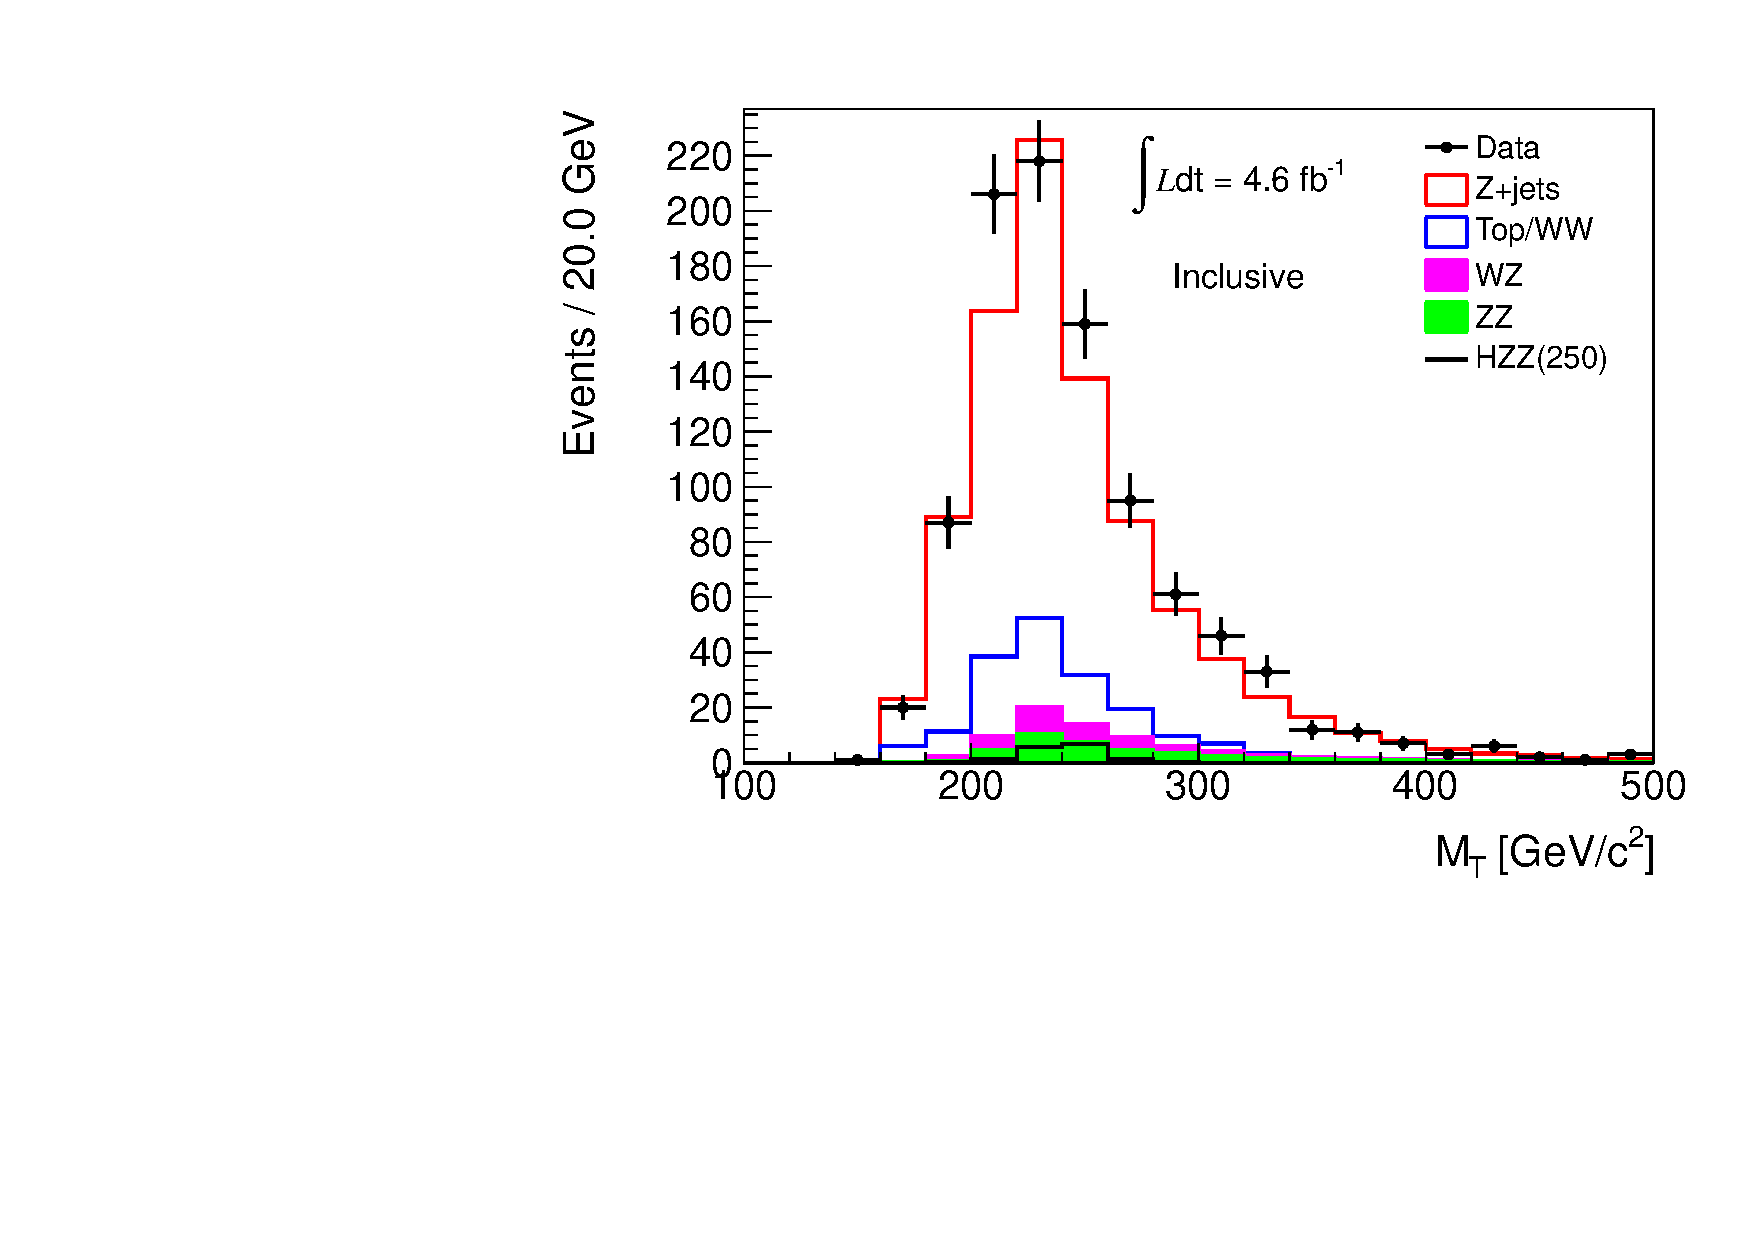
\includegraphics[width=.4\textwidth]{figures/presel_mH250_ee_mt_incl.pdf}}
\subfigure[0-Jet]{\label{subfig:mt_ee_0j}
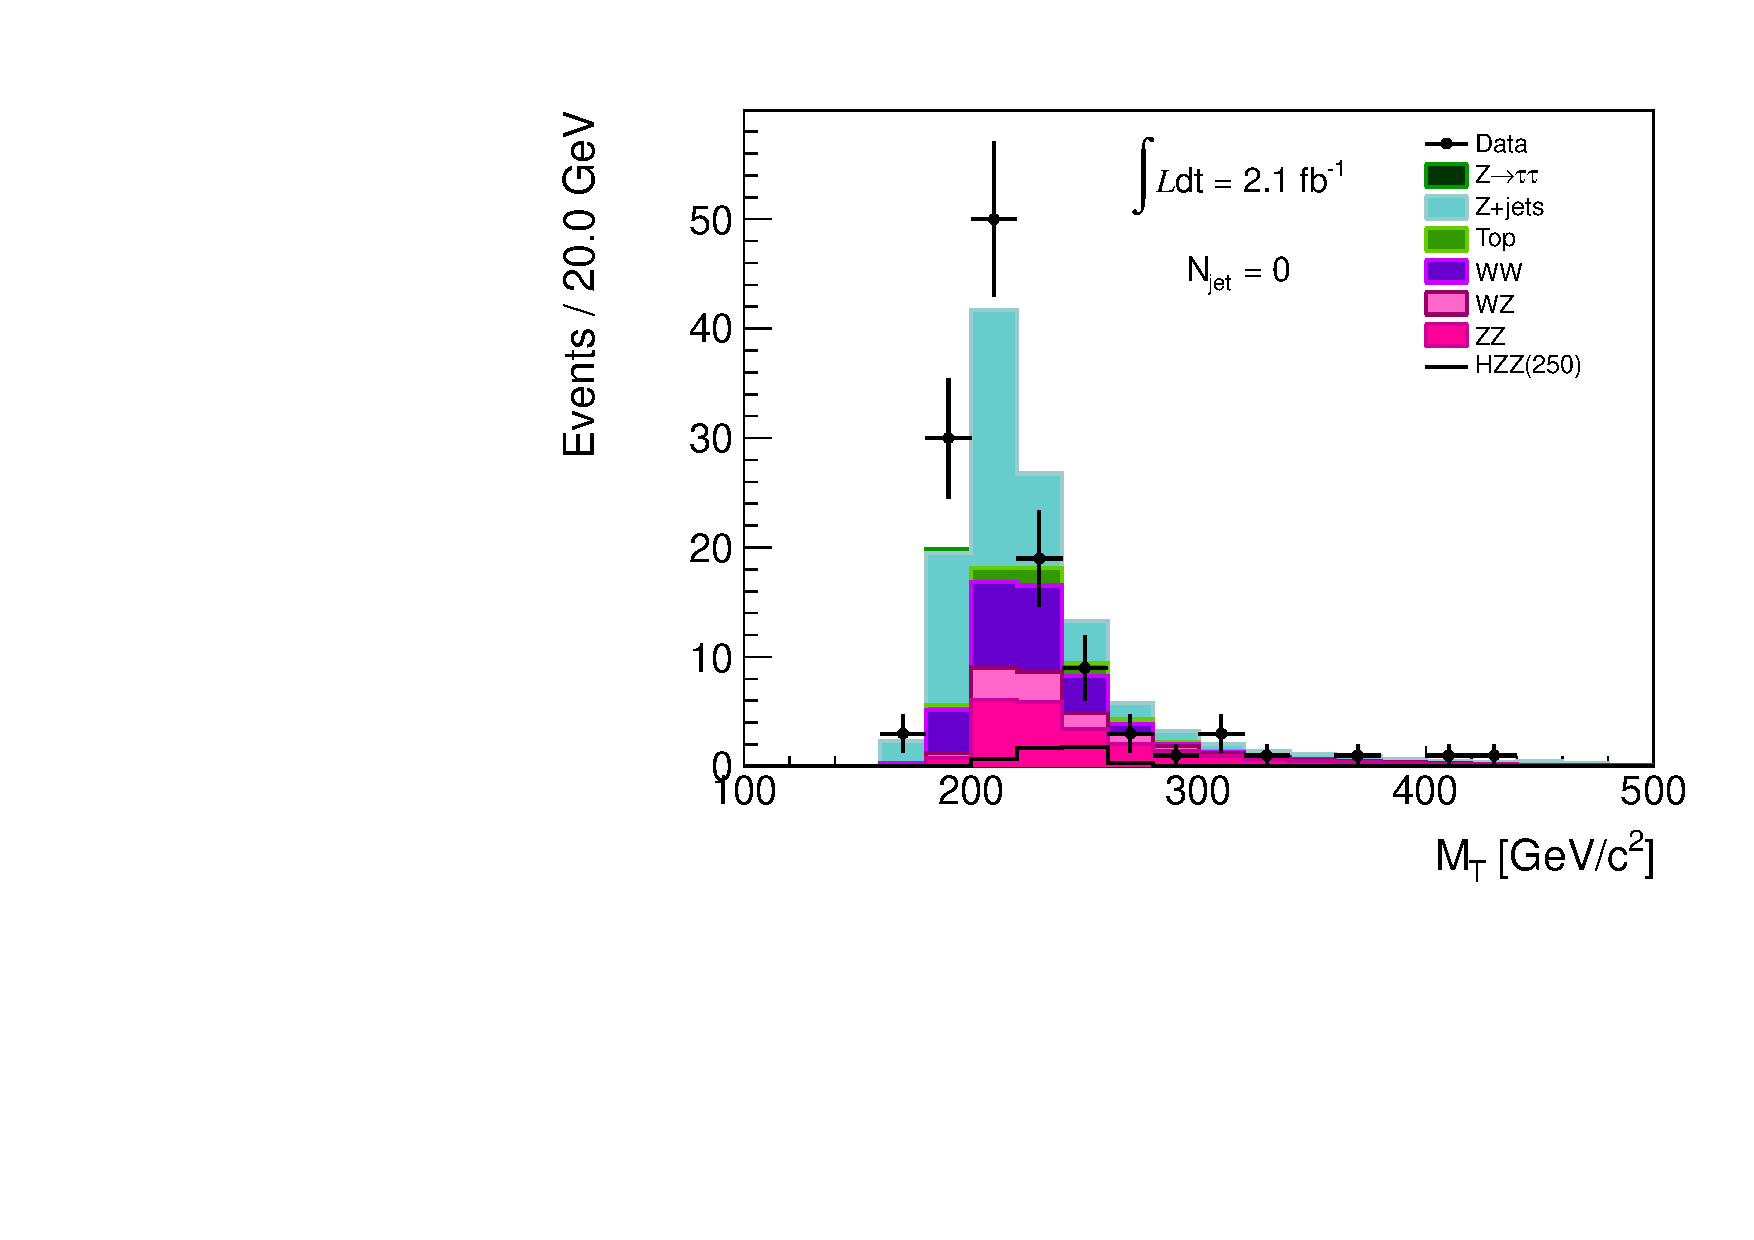
\includegraphics[width=.4\textwidth]{figures/presel_mH250_ee_mt_0j.pdf}} \\
\subfigure[1-Jet]{\label{subfig:mt_ee_1j}
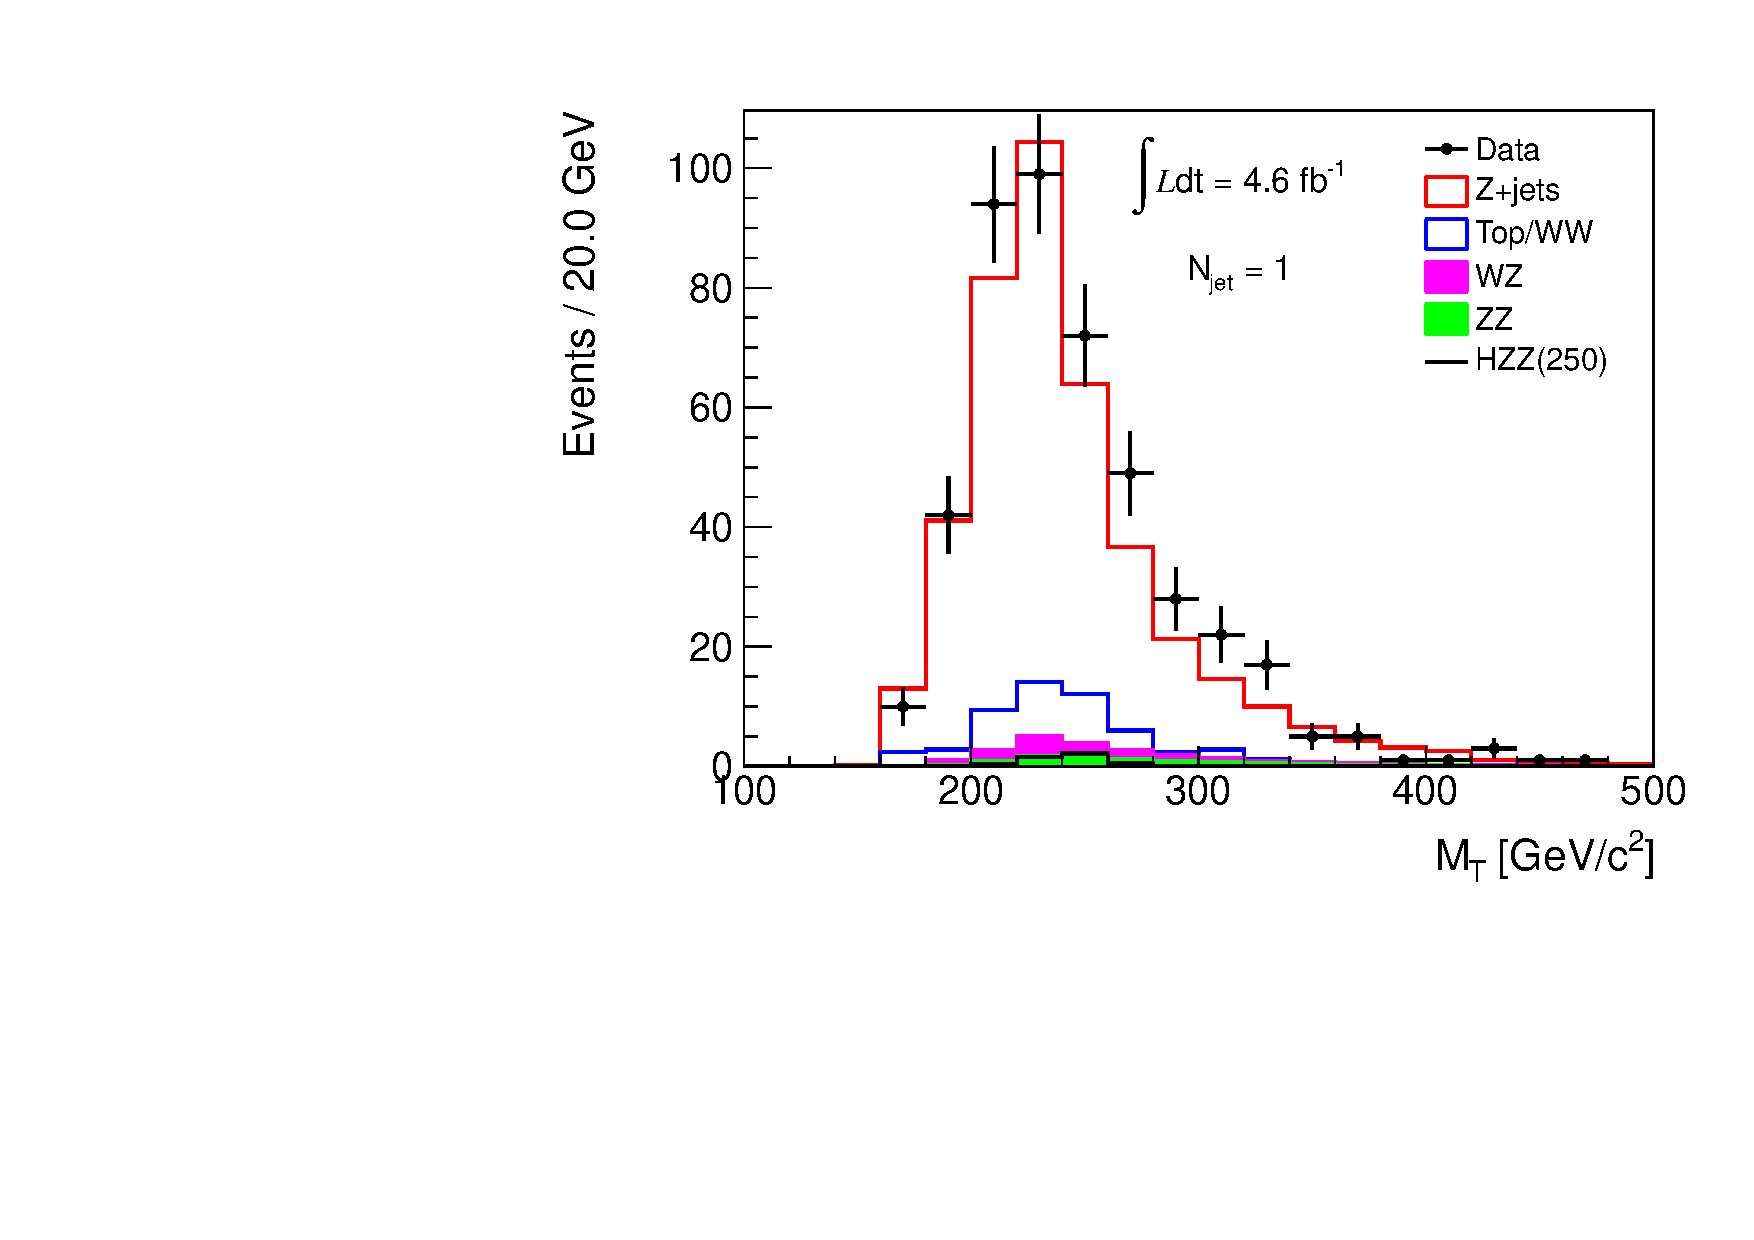
\includegraphics[width=.4\textwidth]{figures/presel_mH250_ee_mt_1j.pdf}}
\subfigure[$\geq$2 Jets]{\label{subfig:mt_ee_2j}
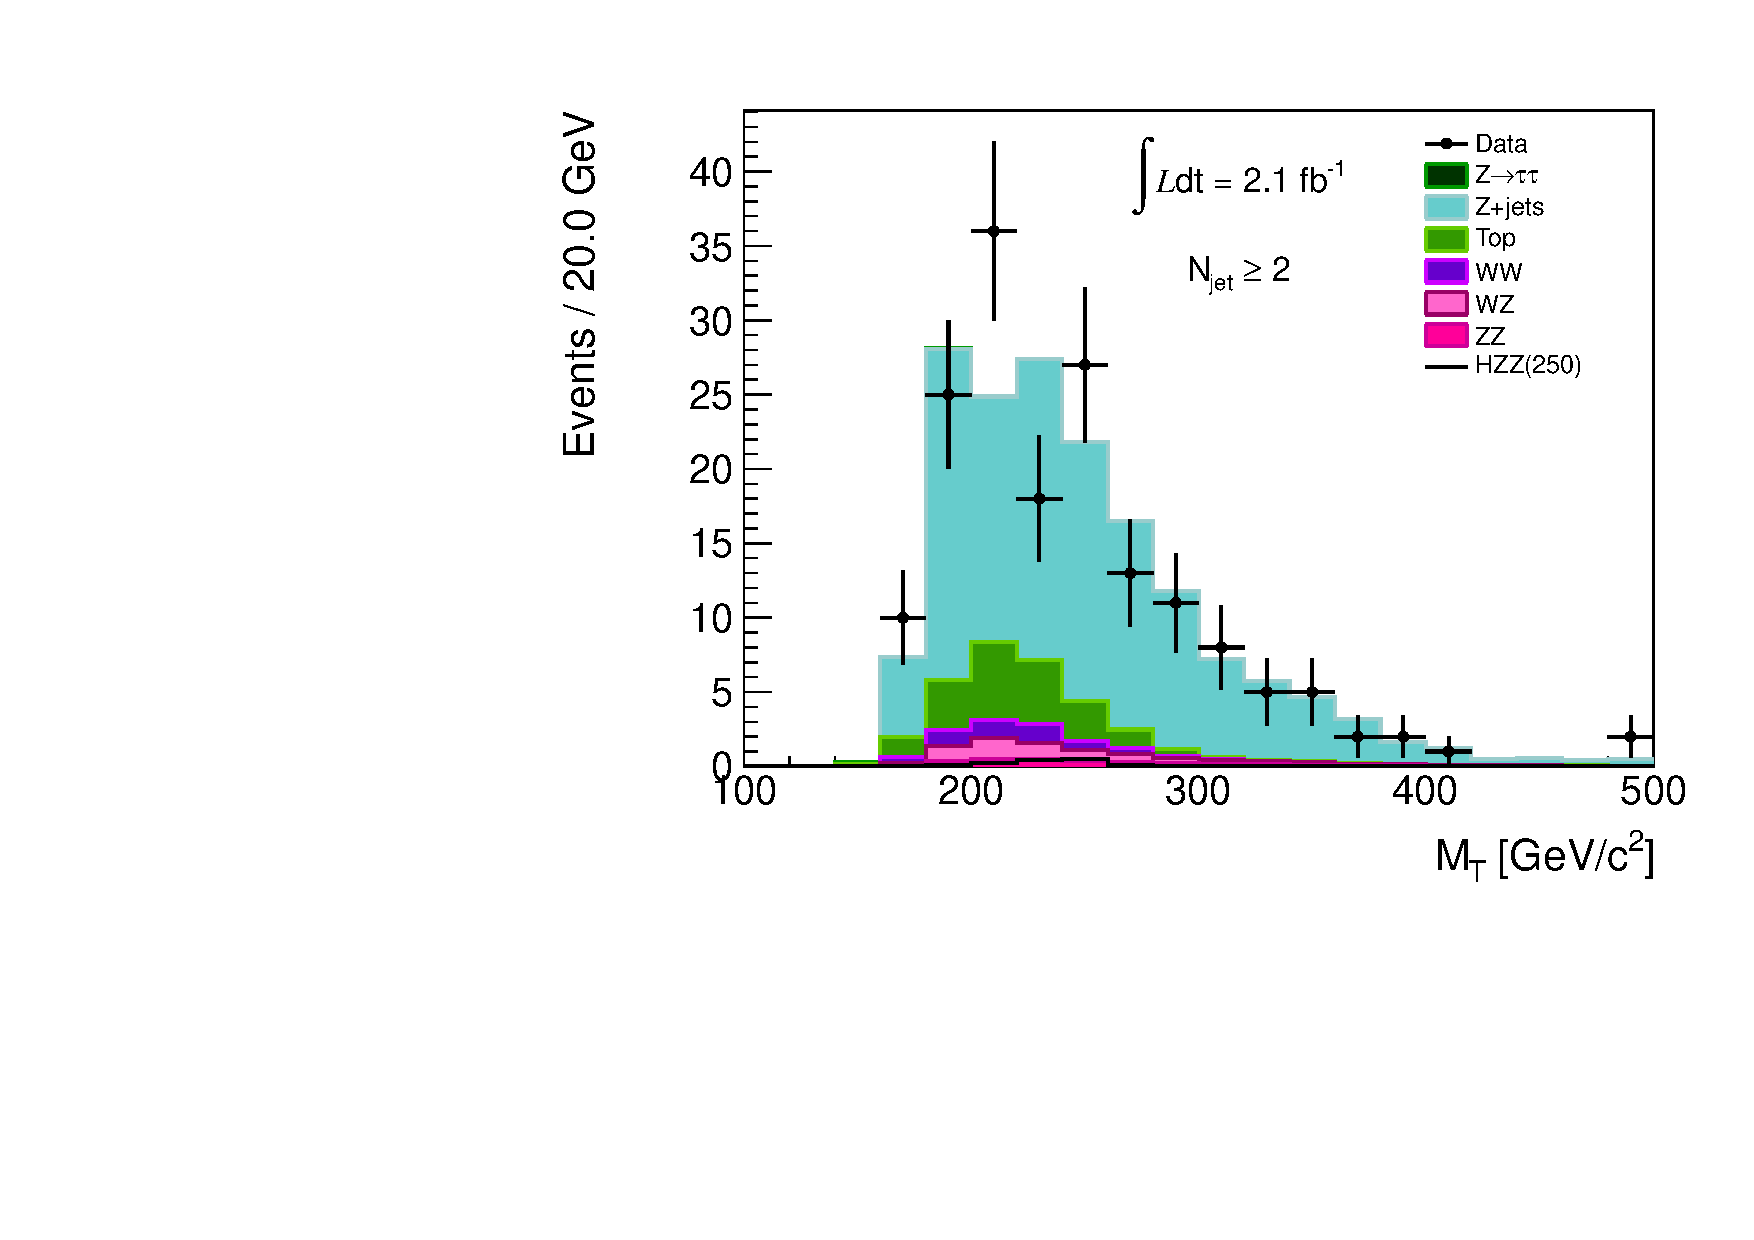
\includegraphics[width=.4\textwidth]{figures/presel_mH250_ee_mt_2j.pdf}}
\caption{Transverse mass distribution in the electron channel after the $\ZZ$ preselection observed in data corresponding to $2.1$~\ifb data in 
the Inclusive~\subref{subfig:mt_ee_incl}, 0-Jet~\subref{subfig:mt_ee_0j}, 1-Jet~\subref{subfig:mt_ee_1j} and 2-Jet~\subref{subfig:mt_ee_2j} bins, 
compared to the expected from simulation for signal and background. The MC backgrounds are scaled as appropriate and the photon+jets estimate of the 
Z+jets background is added to the stack.}
\label{fig:mt_zzpresel_ee}
\end{center}
\end{figure}
%%%%%%%%

%%%%%%%%
\begin{figure}[!hbtp]
\begin{center}
\subfigure[Inclusive]{\label{subfig:dphijetmet_mm_incl}
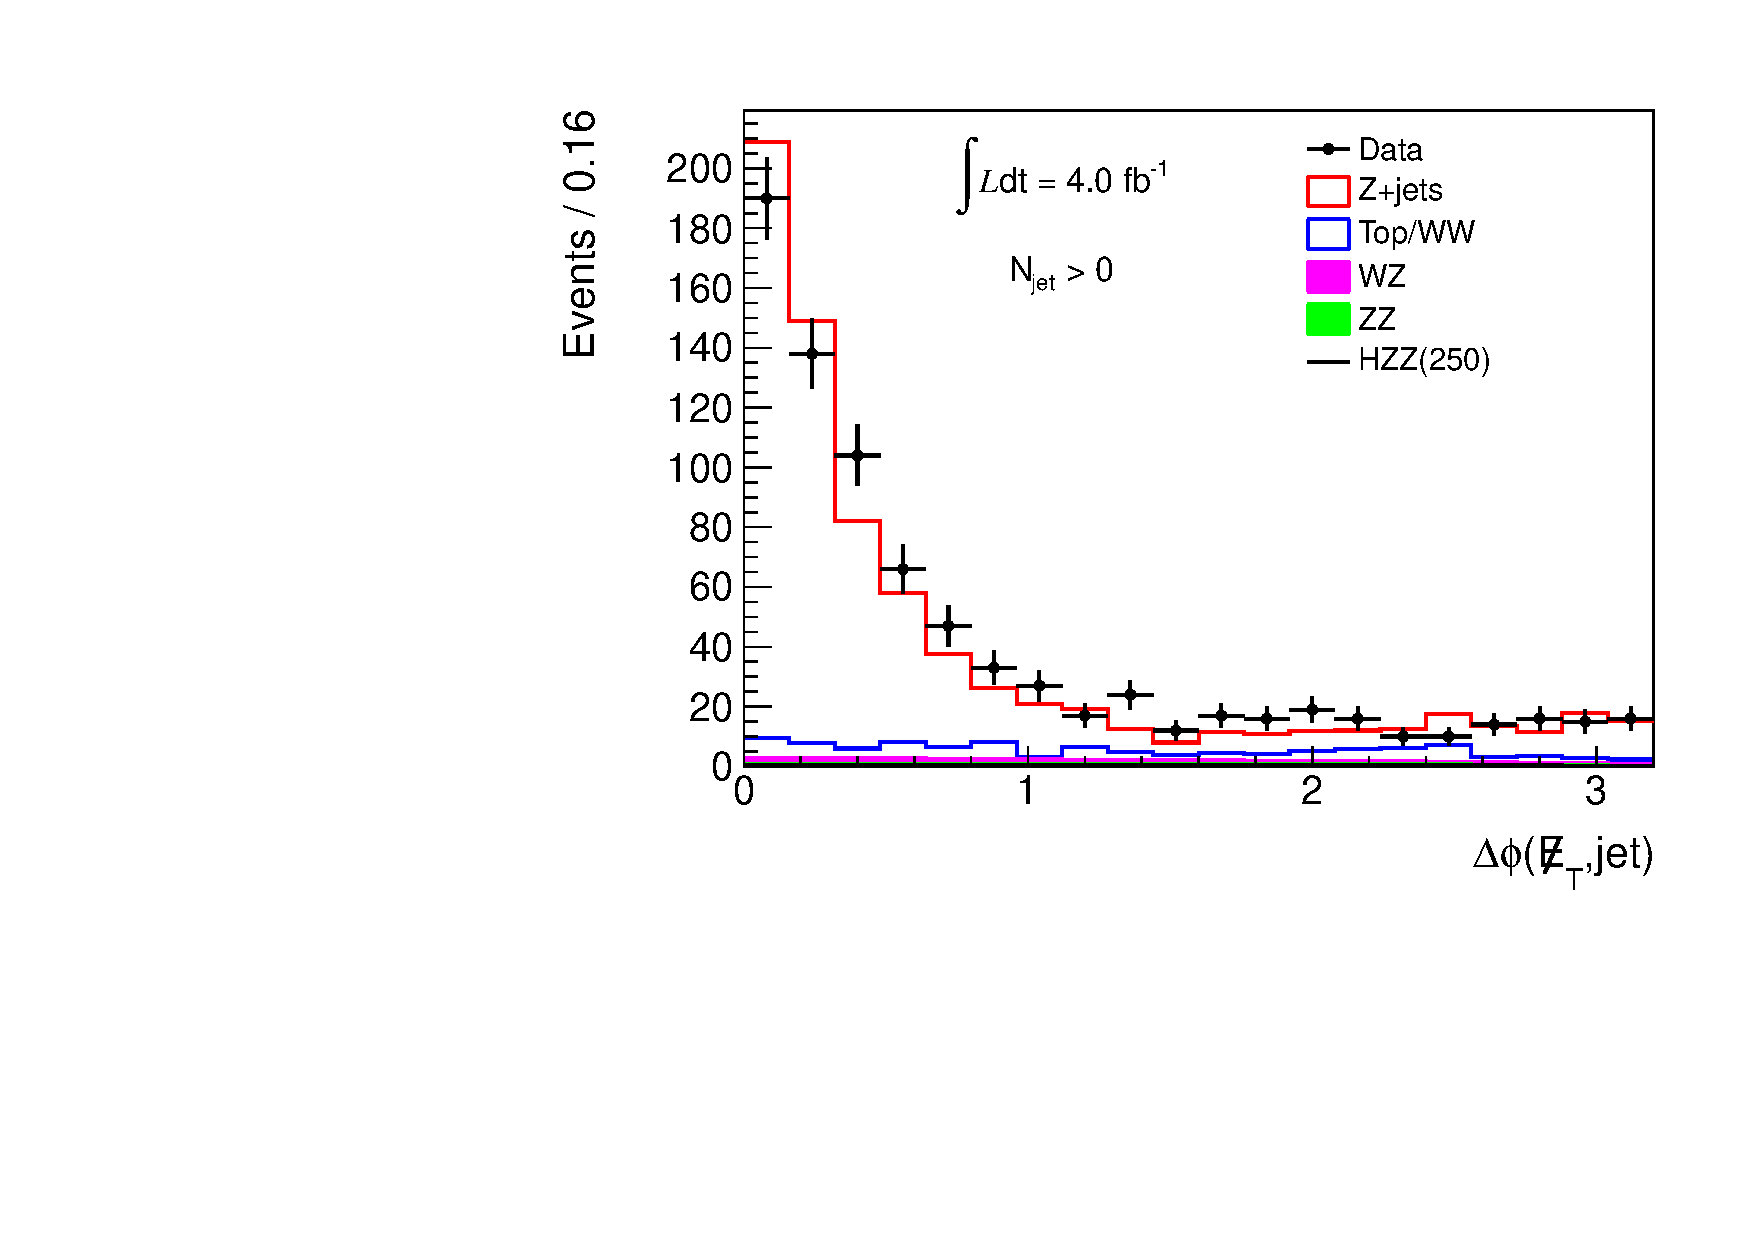
\includegraphics[width=.3\textwidth]{figures/presel_mH250_mm_dphijetmet_incl.pdf}}
\subfigure[1-Jet]{\label{subfig:dphijetmet_mm_1j}
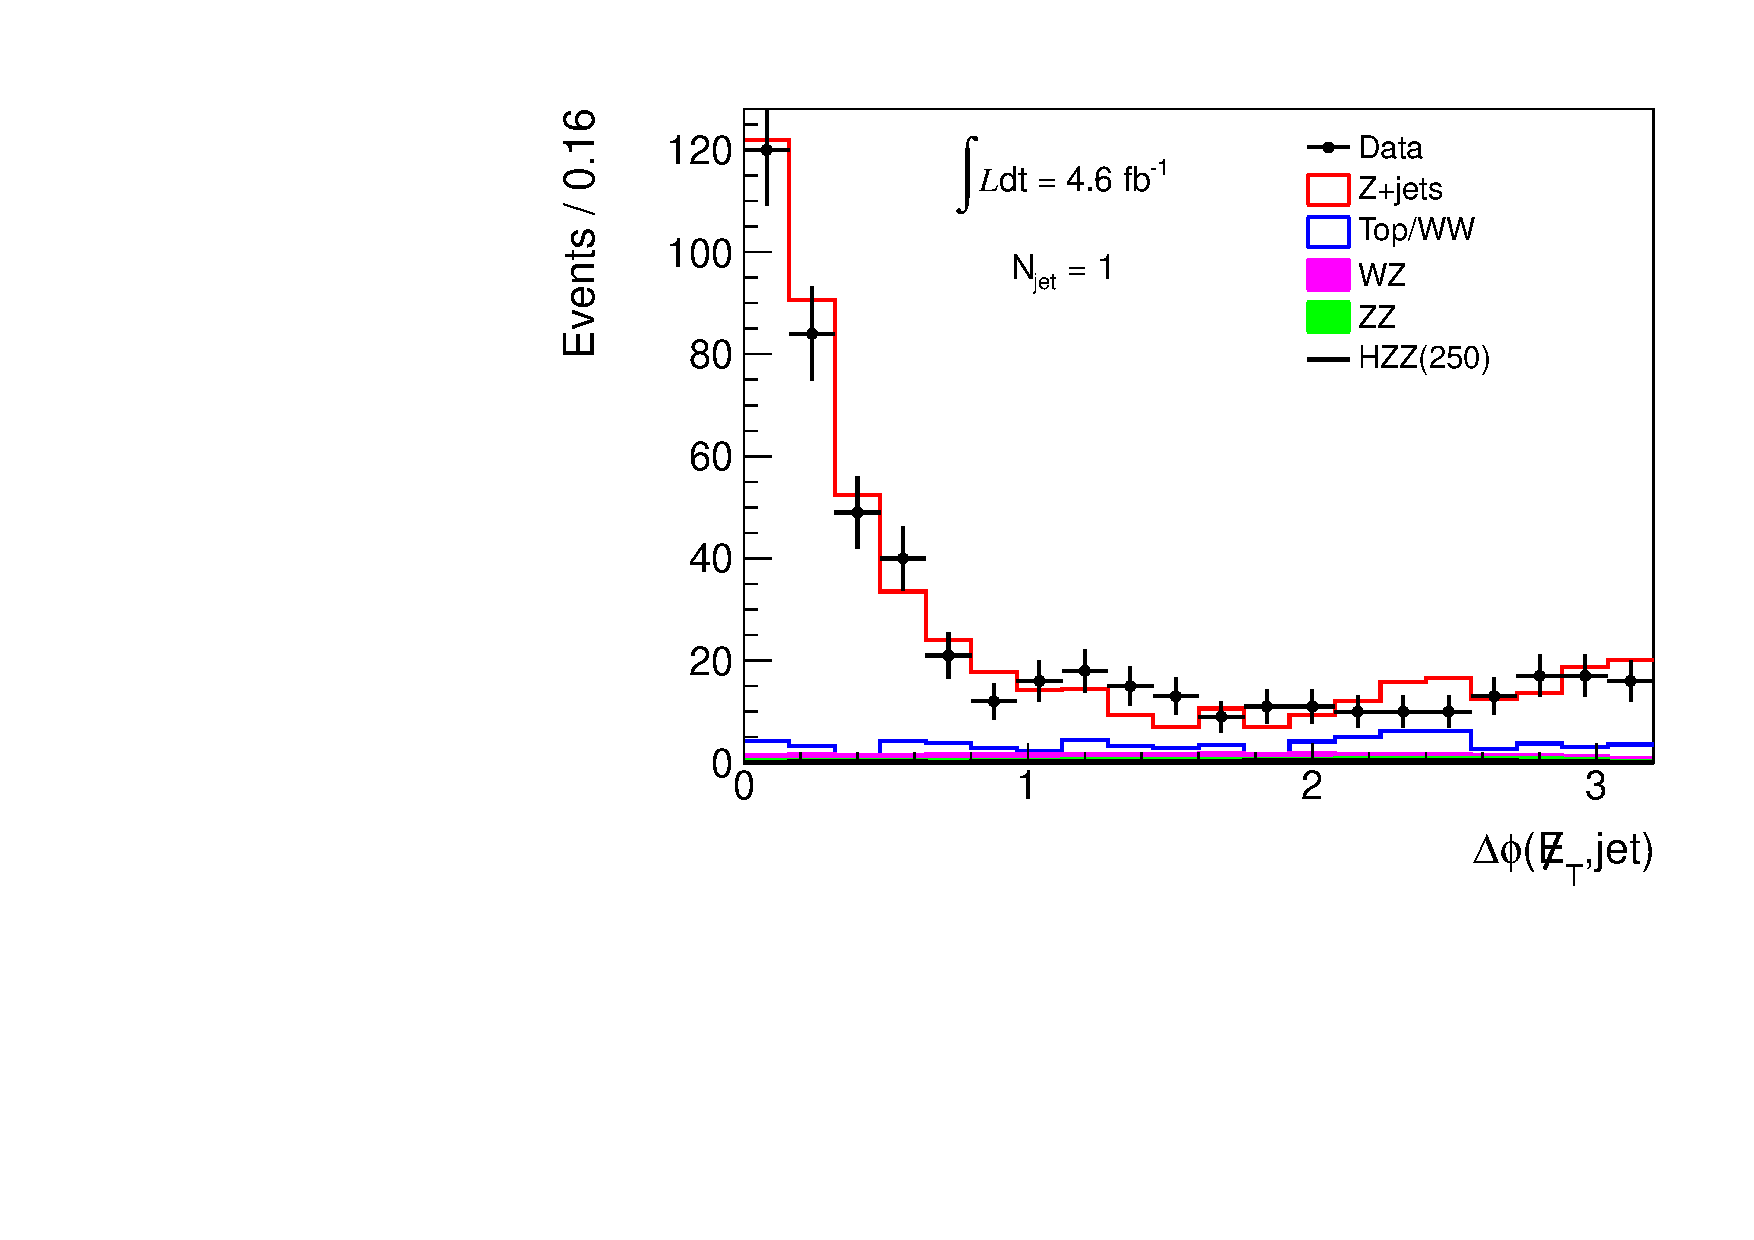
\includegraphics[width=.3\textwidth]{figures/presel_mH250_mm_dphijetmet_1j.pdf}}
\subfigure[$\geq$2 Jets]{\label{subfig:dphijetmet_mm_2j}
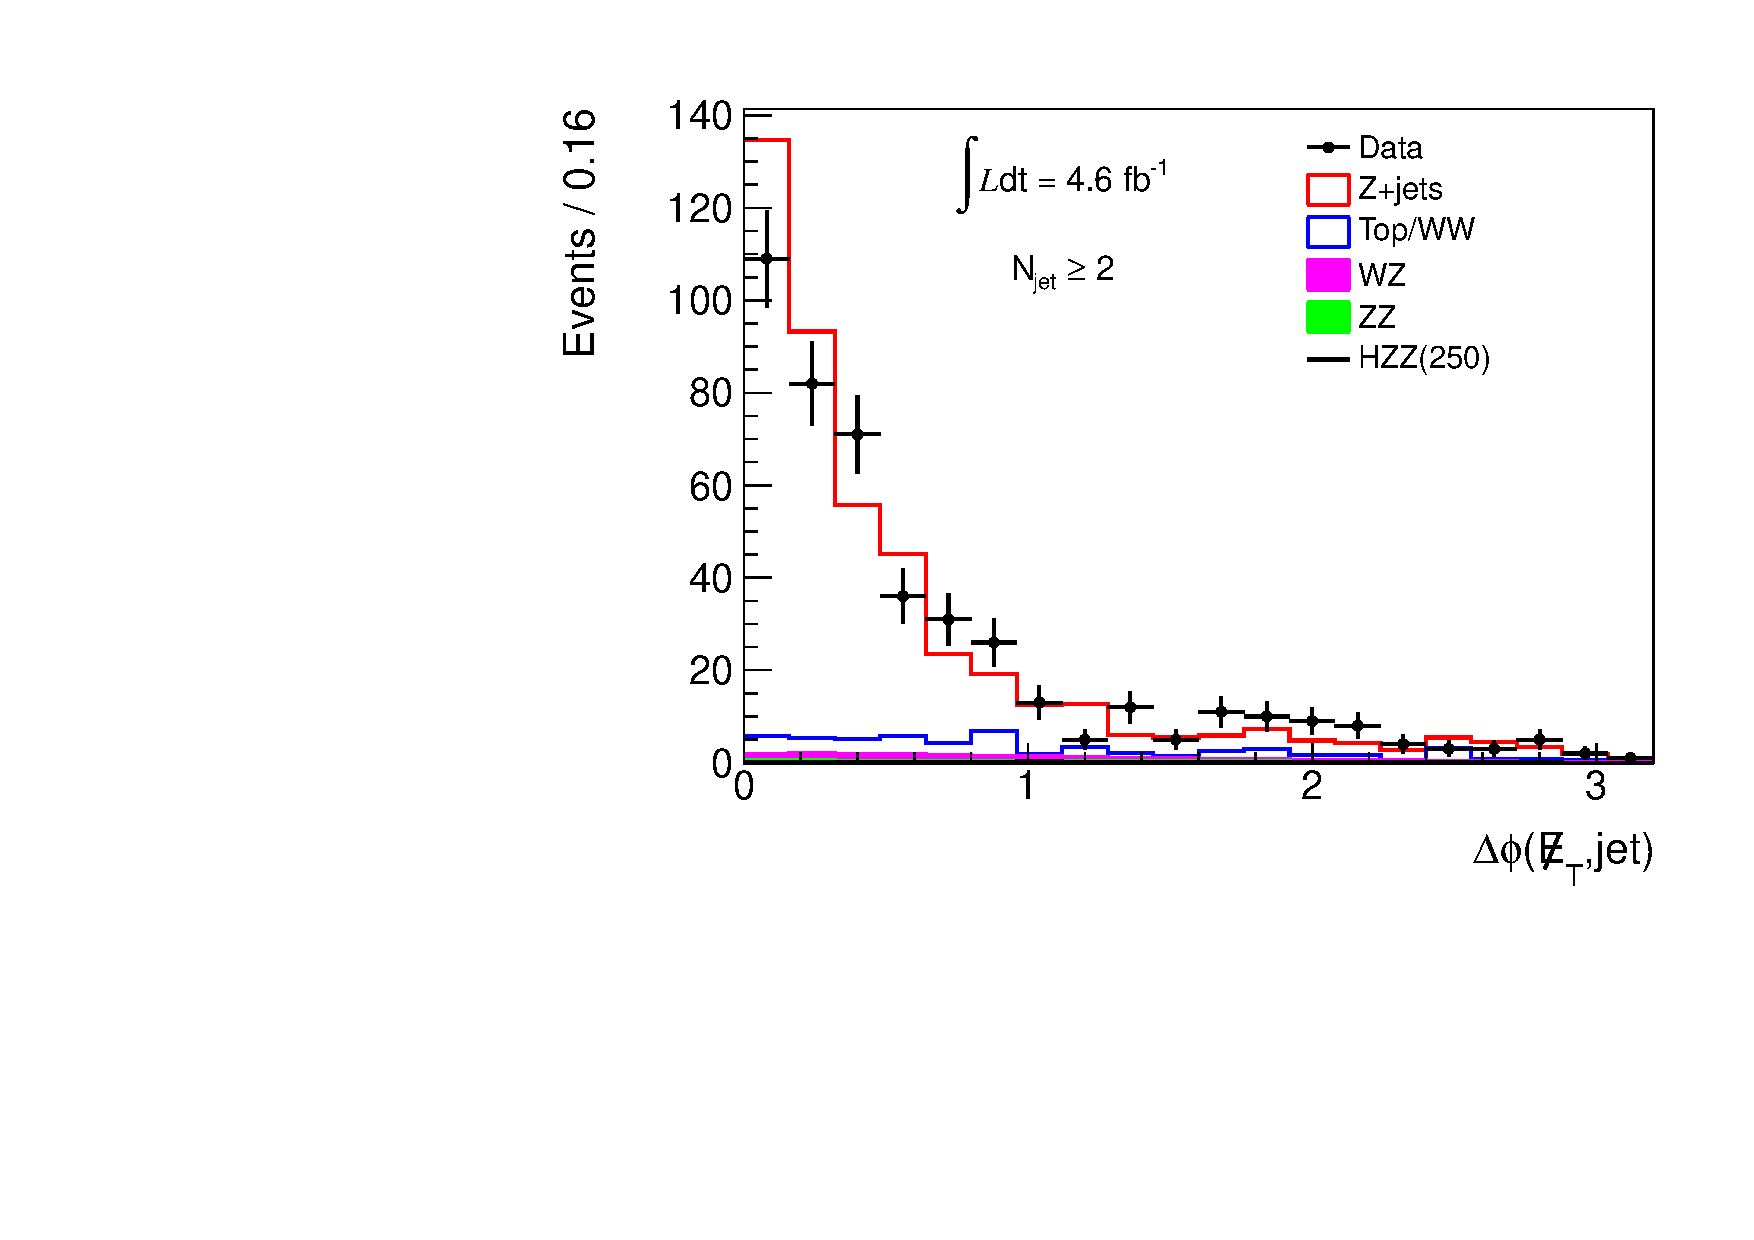
\includegraphics[width=.3\textwidth]{figures/presel_mH250_mm_dphijetmet_2j.pdf}}
\caption{Azimuthal angle separation between \met and the closest jet in the muon channel after the $\ZZ$ preselection observed in data corresponding 
to $2.1$~\ifb data in the Inclusive~\subref{subfig:dphijetmet_mm_incl}, 1-Jet~\subref{subfig:dphijetmet_mm_1j} and 
2-Jet~\subref{subfig:dphijetmet_mm_2j} bins, compared to the expected from simulation for signal and background. The MC backgrounds are scaled as appropriate and 
the photon+jets estimate of the Z+jets background is added to the stack.}
\label{fig:dphijetmet_zzpresel_mm}
\end{center}
\end{figure}
%%%%%%%%

%%%%%%%%
\begin{figure}[!hbtp]
\begin{center}
\subfigure[Inclusive]{\label{subfig:dphijetmet_ee_incl}
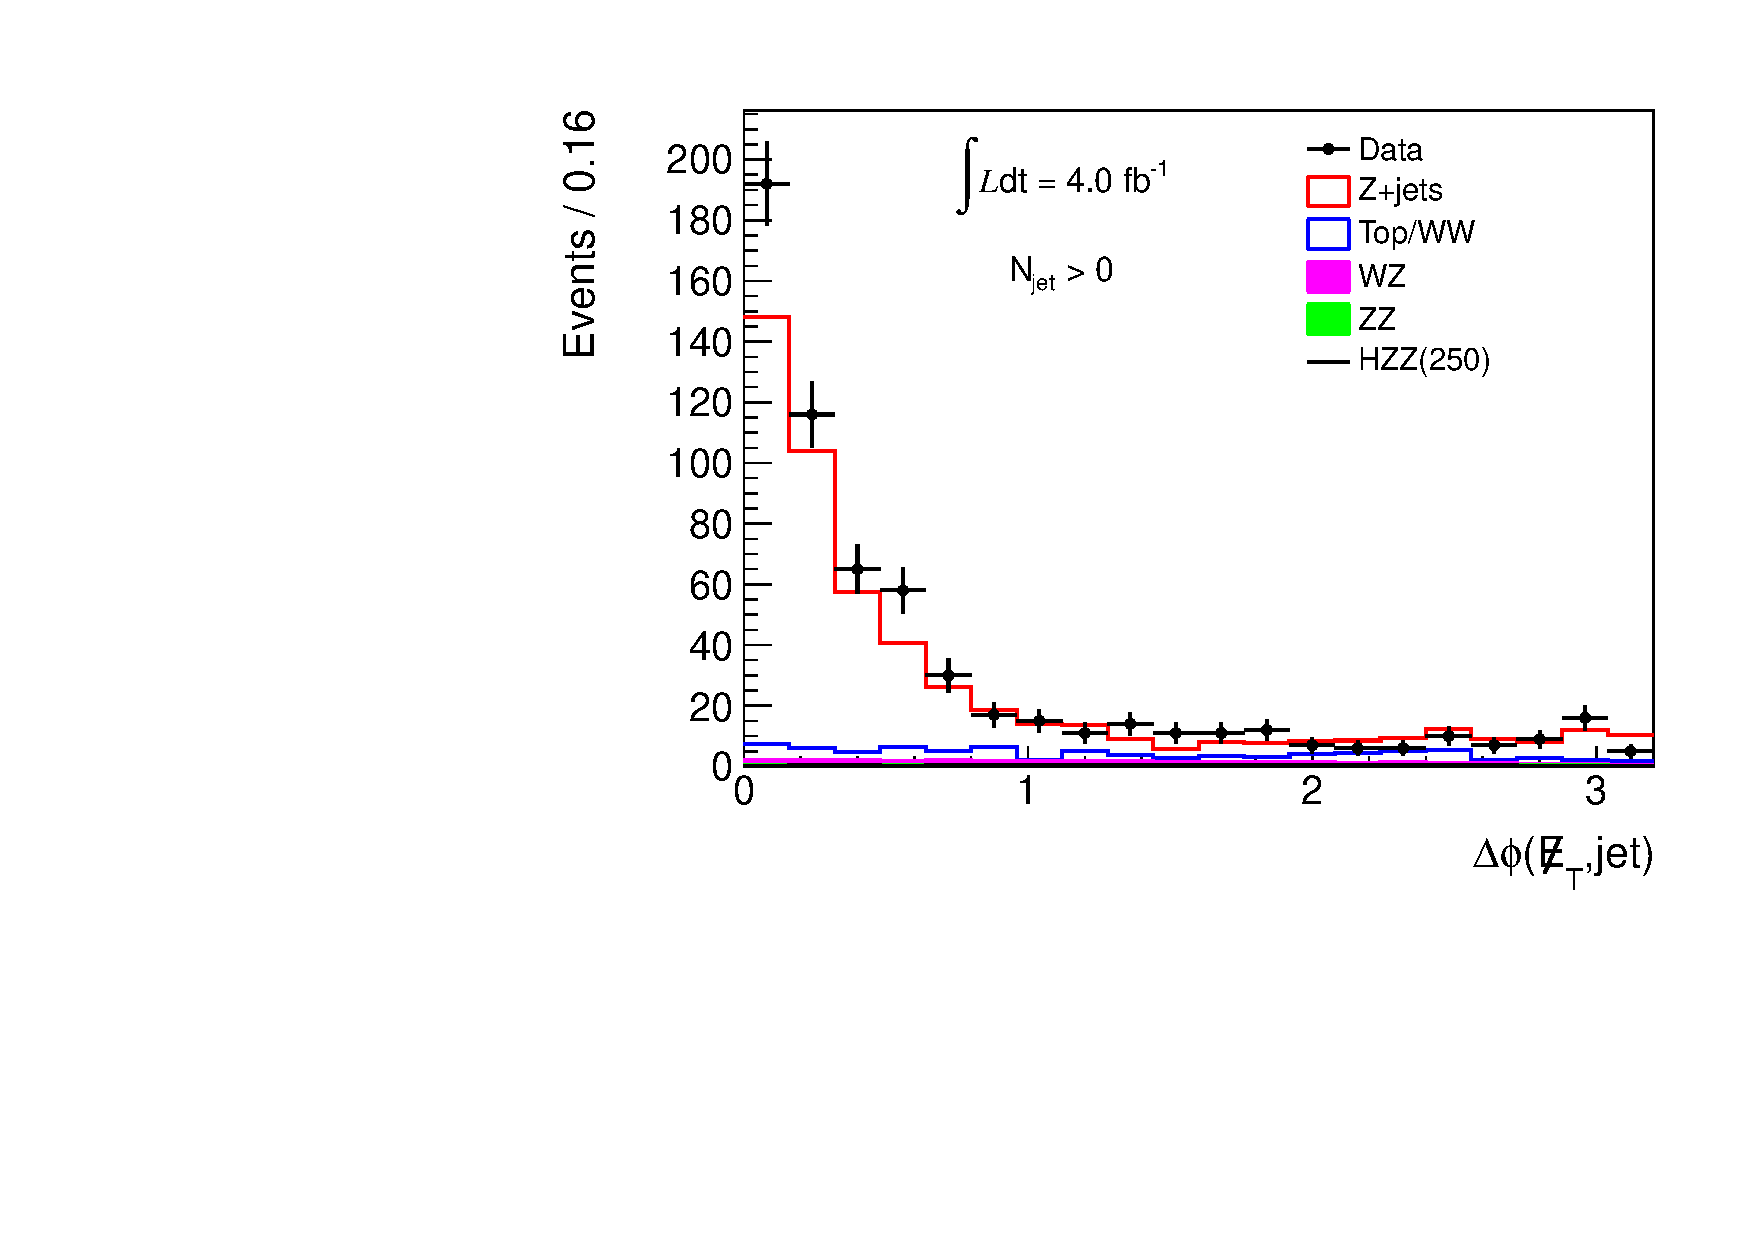
\includegraphics[width=.3\textwidth]{figures/presel_mH250_ee_dphijetmet_incl.pdf}}
\subfigure[1-Jet]{\label{subfig:dphijetmet_ee_1j}
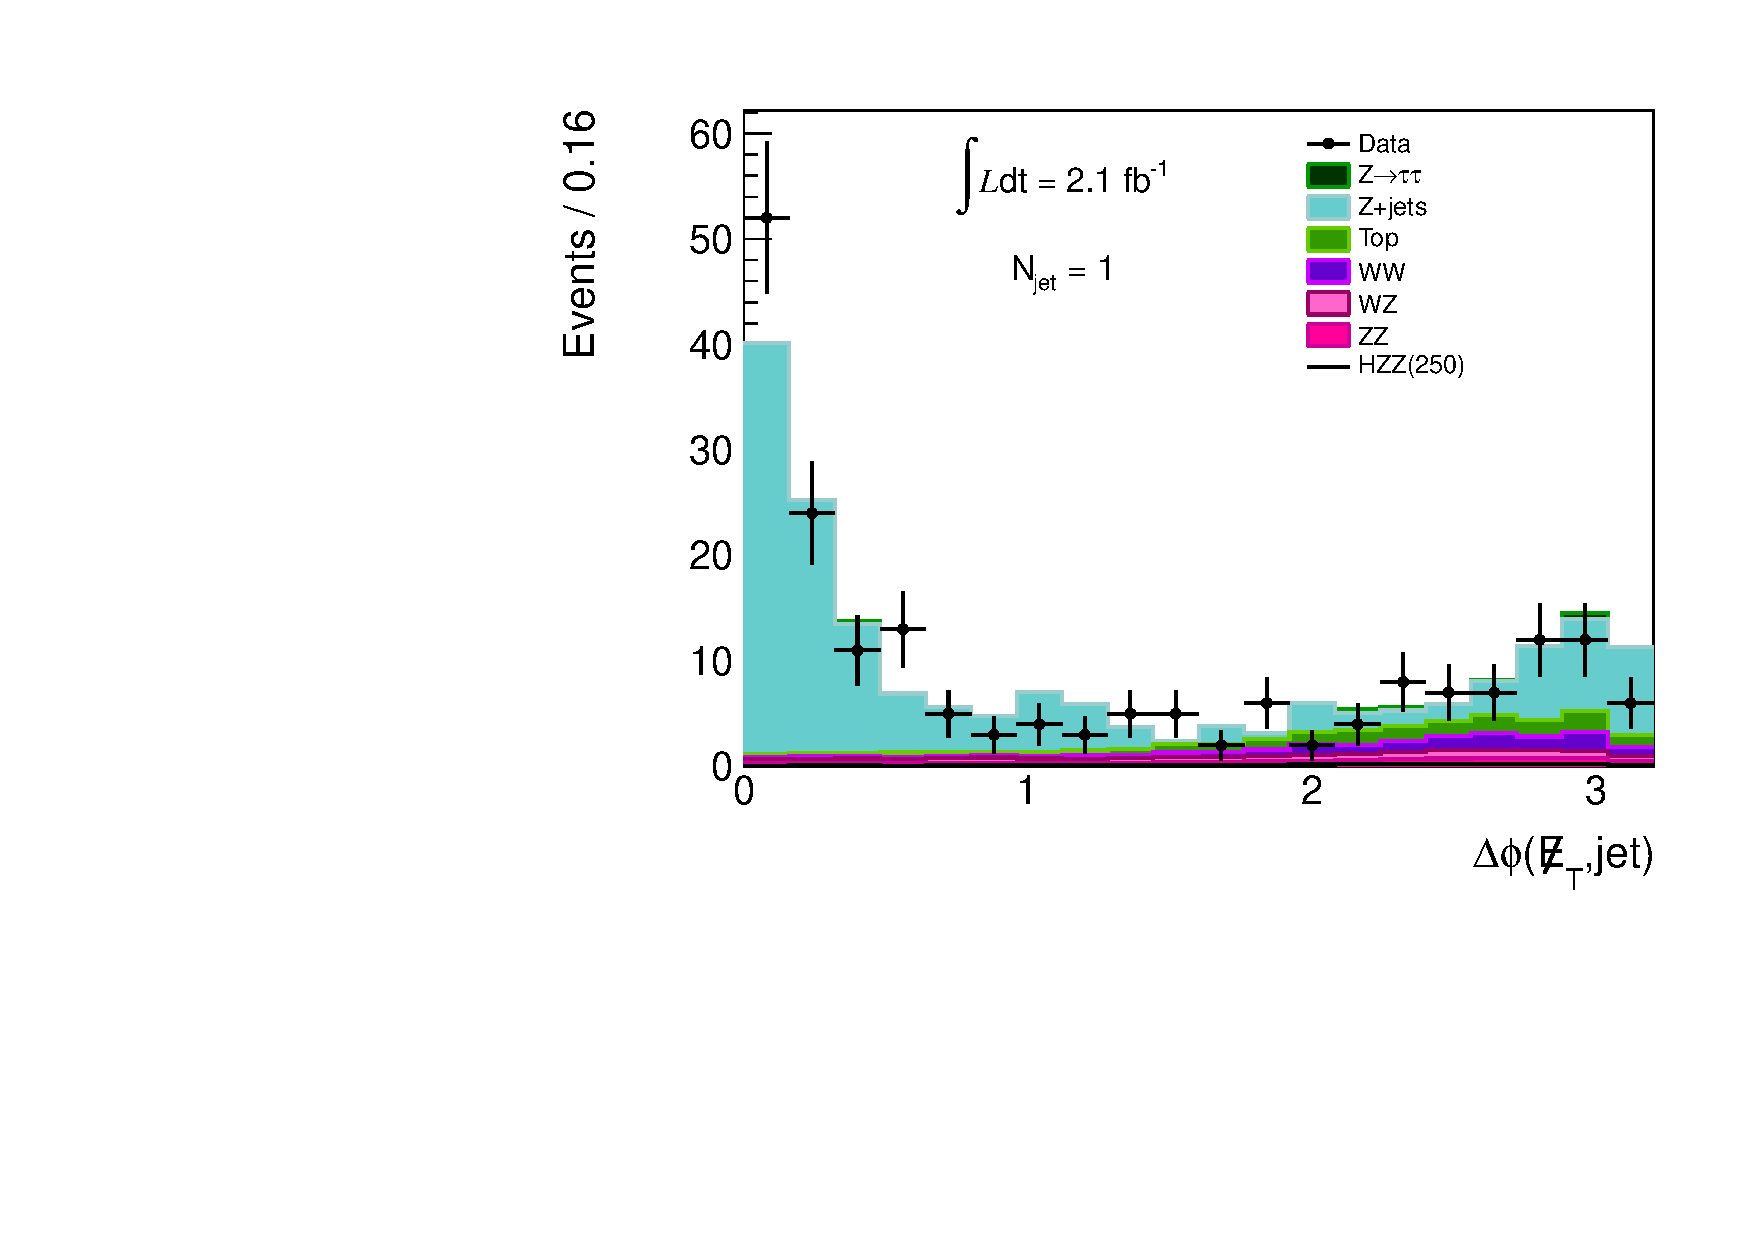
\includegraphics[width=.3\textwidth]{figures/presel_mH250_ee_dphijetmet_1j.pdf}}
\subfigure[$\geq$2 Jets]{\label{subfig:dphijetmet_ee_2j}
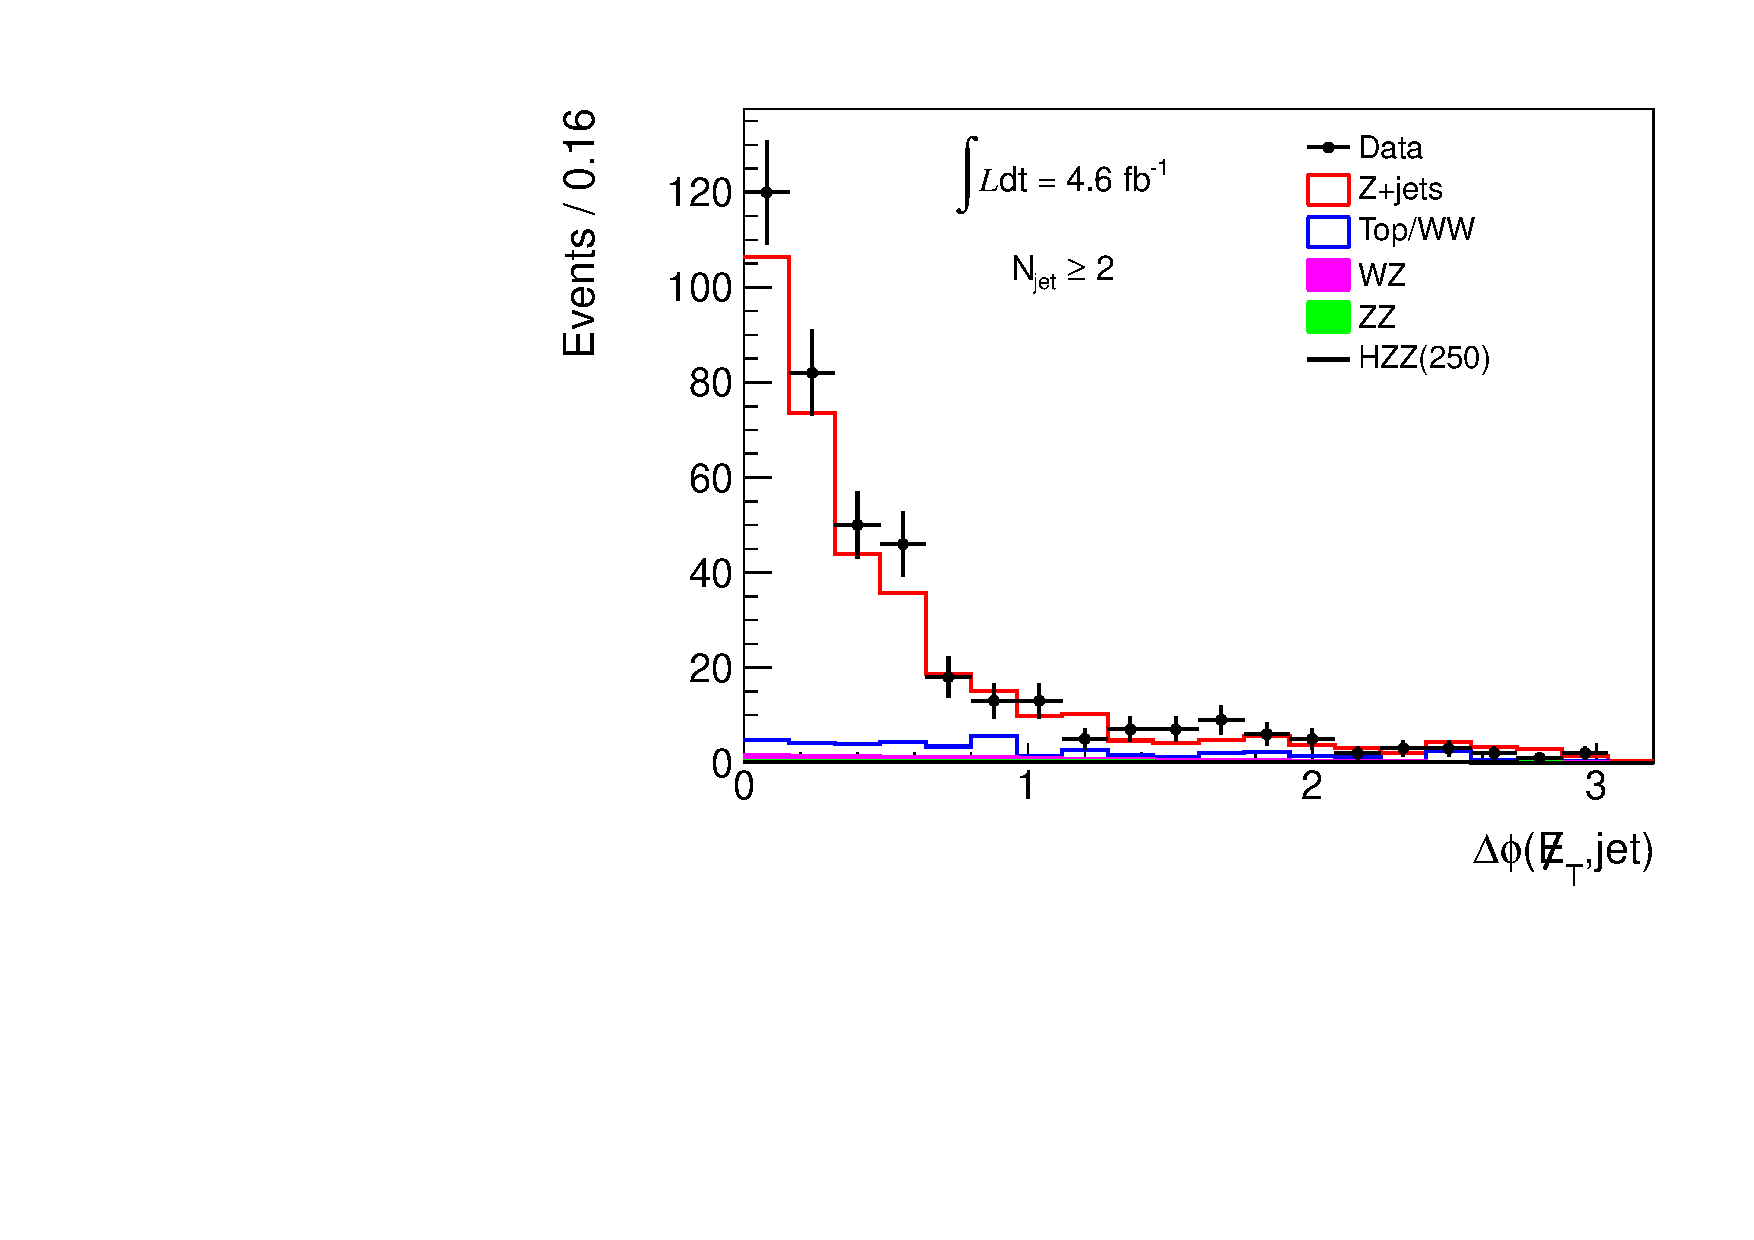
\includegraphics[width=.3\textwidth]{figures/presel_mH250_ee_dphijetmet_2j.pdf}}
\caption{Azimuthal angle separation between \met and the closest jet in the electron channel after the $\ZZ$ preselection observed in data corresponding 
to $2.1$~\ifb data in the Inclusive~\subref{subfig:dphijetmet_mm_incl}, 1-Jet~\subref{subfig:dphijetmet_mm_1j} and 
2-Jet~\subref{subfig:dphijetmet_mm_2j} bins, compared to the expected from simulation for signal and background. The MC backgrounds are scaled as appropriate and 
the photon+jets estimate of the Z+jets background is added to the stack.}
\label{fig:dphijetmet_zzpresel_ee}
\end{center}
\end{figure}
%%%%%%%%





\clearpage

\subsection{Results in the Top/WW control region}
\label{sec:results_topww}
We define a control region enriched in top and $WW$ events to validate our method to estimate those backgrounds
with opposite flavor dilepton events. The selection criteria are the following:
\begin{itemize}
\item $|m_{\ell\ell} - m_Z| > 15\:\GeVcc$,
\item $M_T > 150\:\GeVcc$,
\item MET > threshold for the $m_H=250\:\GeVcc$ selection,
\item $\Delta\phi\left(\mbox{jet},\mbox{MET}\right)$ > threshold for the $m_H=250\:\GeVcc$ selection. 
\end{itemize} 


%%%%%%%%
\begin{figure}[!hbtp]
\begin{center}
\subfigure[Inclusive]{\label{subfig:topww_mass_mm}
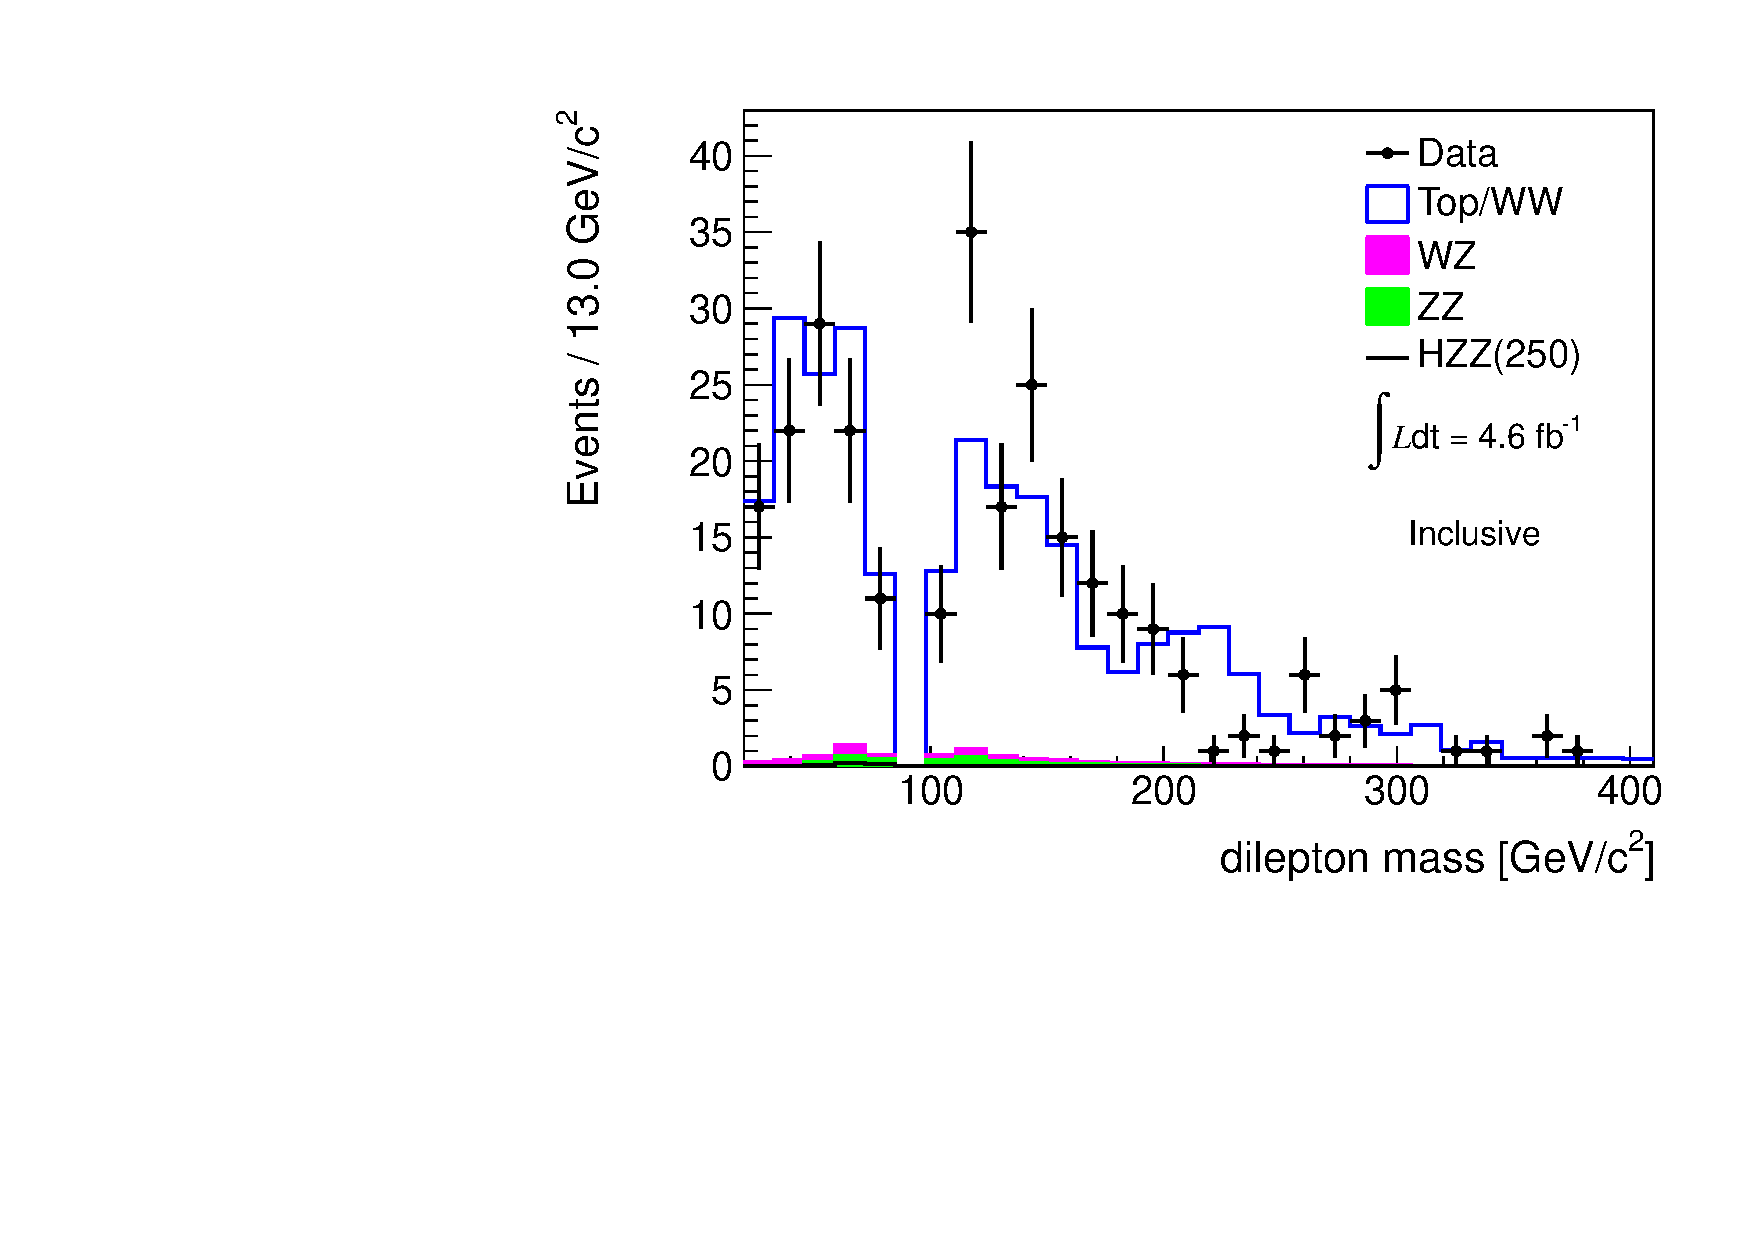
\includegraphics[width=.4\textwidth]{figures/topww_mH250_mm_mass_incl.pdf}}
\subfigure[1-Jet]{\label{subfig:topww_mass_ee}
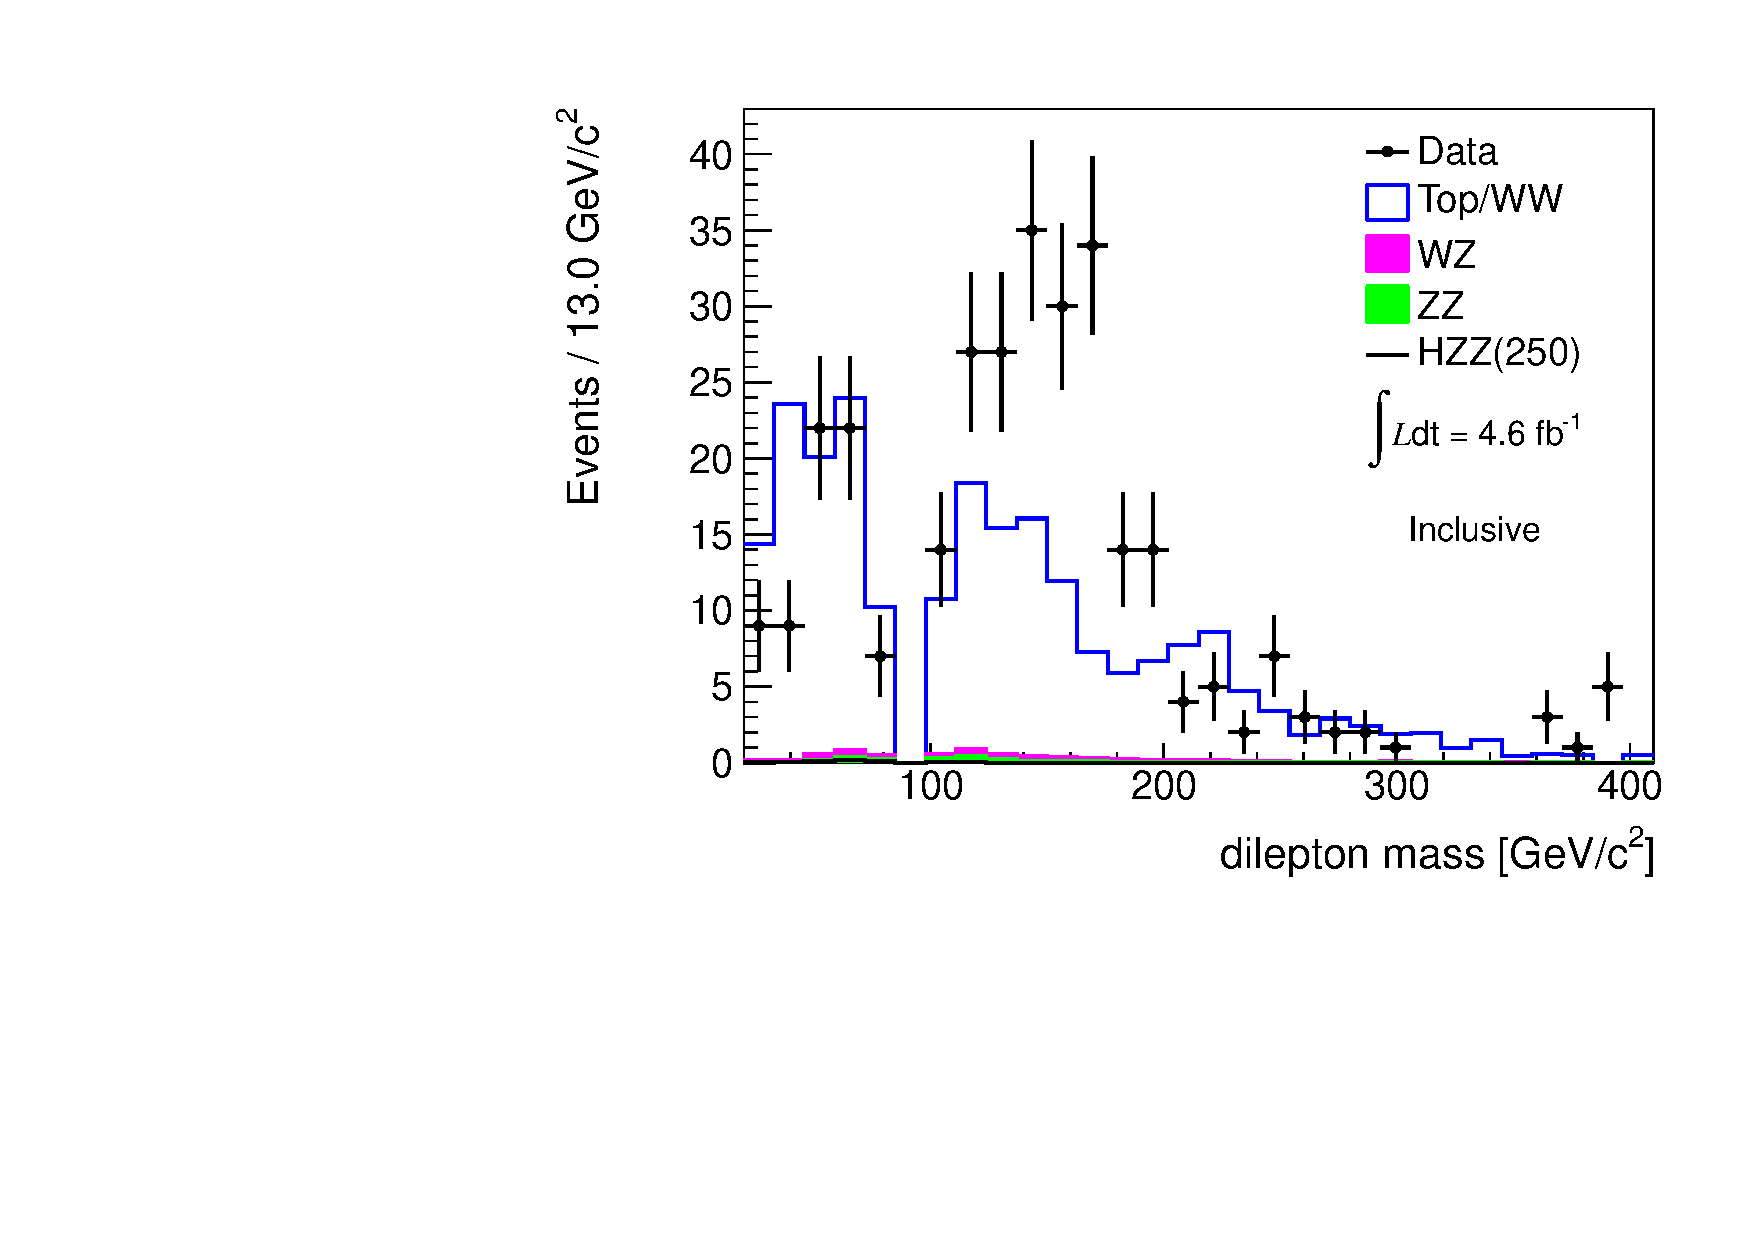
\includegraphics[width=.4\textwidth]{figures/topww_mH250_ee_mass_incl.pdf}}
\caption{Distribution for the dilepton mass in the top/$WW$ control region corresponding 
to $4.0$~\ifb of data in the muon~\subref{subfig:npv_mm} and electron~\subref{subfig:npv_ee} channels, 
compared to the expected from simulation for signal and background. The MC backgrounds are scaled as 
appropriate and the opposite flavor dilepton estimate of the top and $WW$ background is added to the stack.}
\label{fig:topww_mass}
\end{center}
\end{figure}
%%%%%%%%

%%%%%%%%
\begin{figure}[!hbtp]
\begin{center}
\subfigure[Inclusive]{\label{subfig:topww_dileppt_mm}
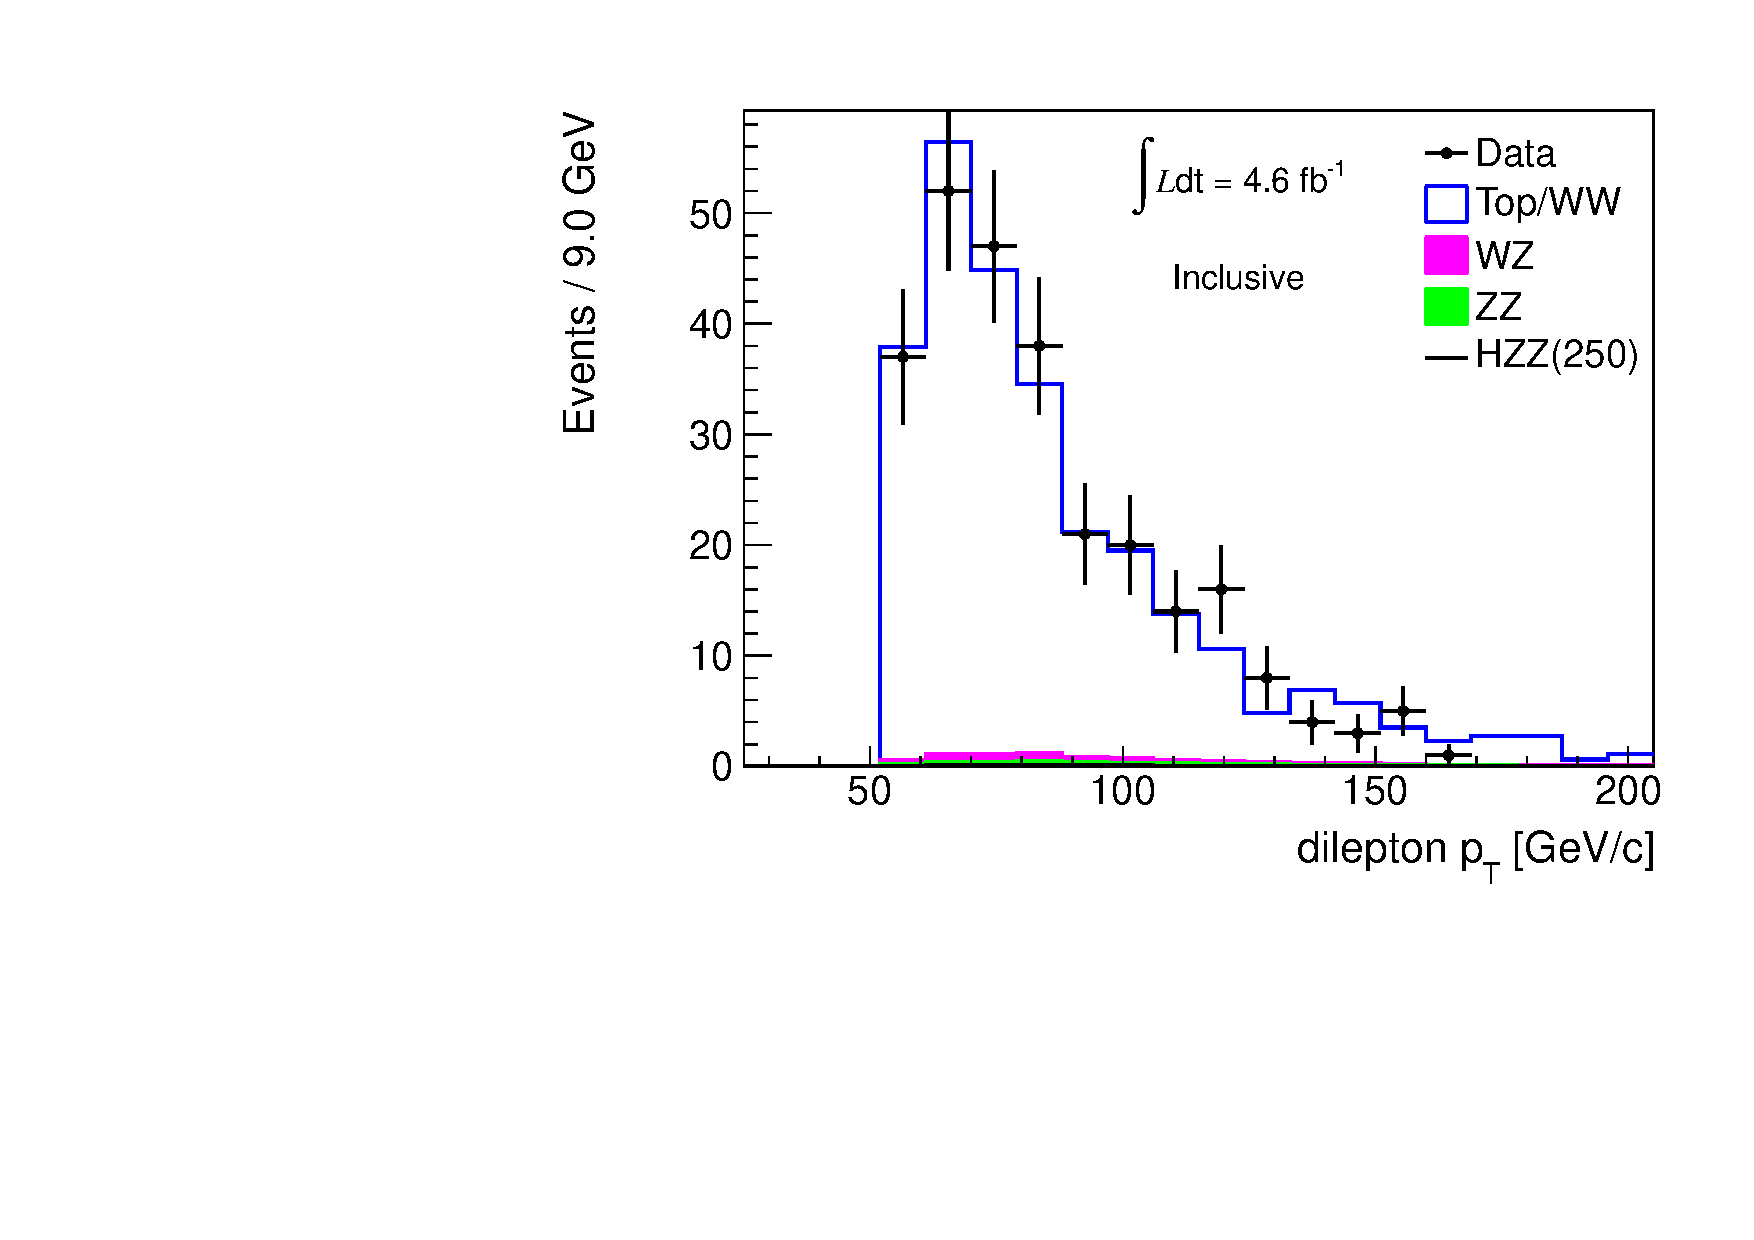
\includegraphics[width=.4\textwidth]{figures/topww_mH250_mm_dileppt_incl.pdf}}
\subfigure[1-Jet]{\label{subfig:topww_dileppt_ee}
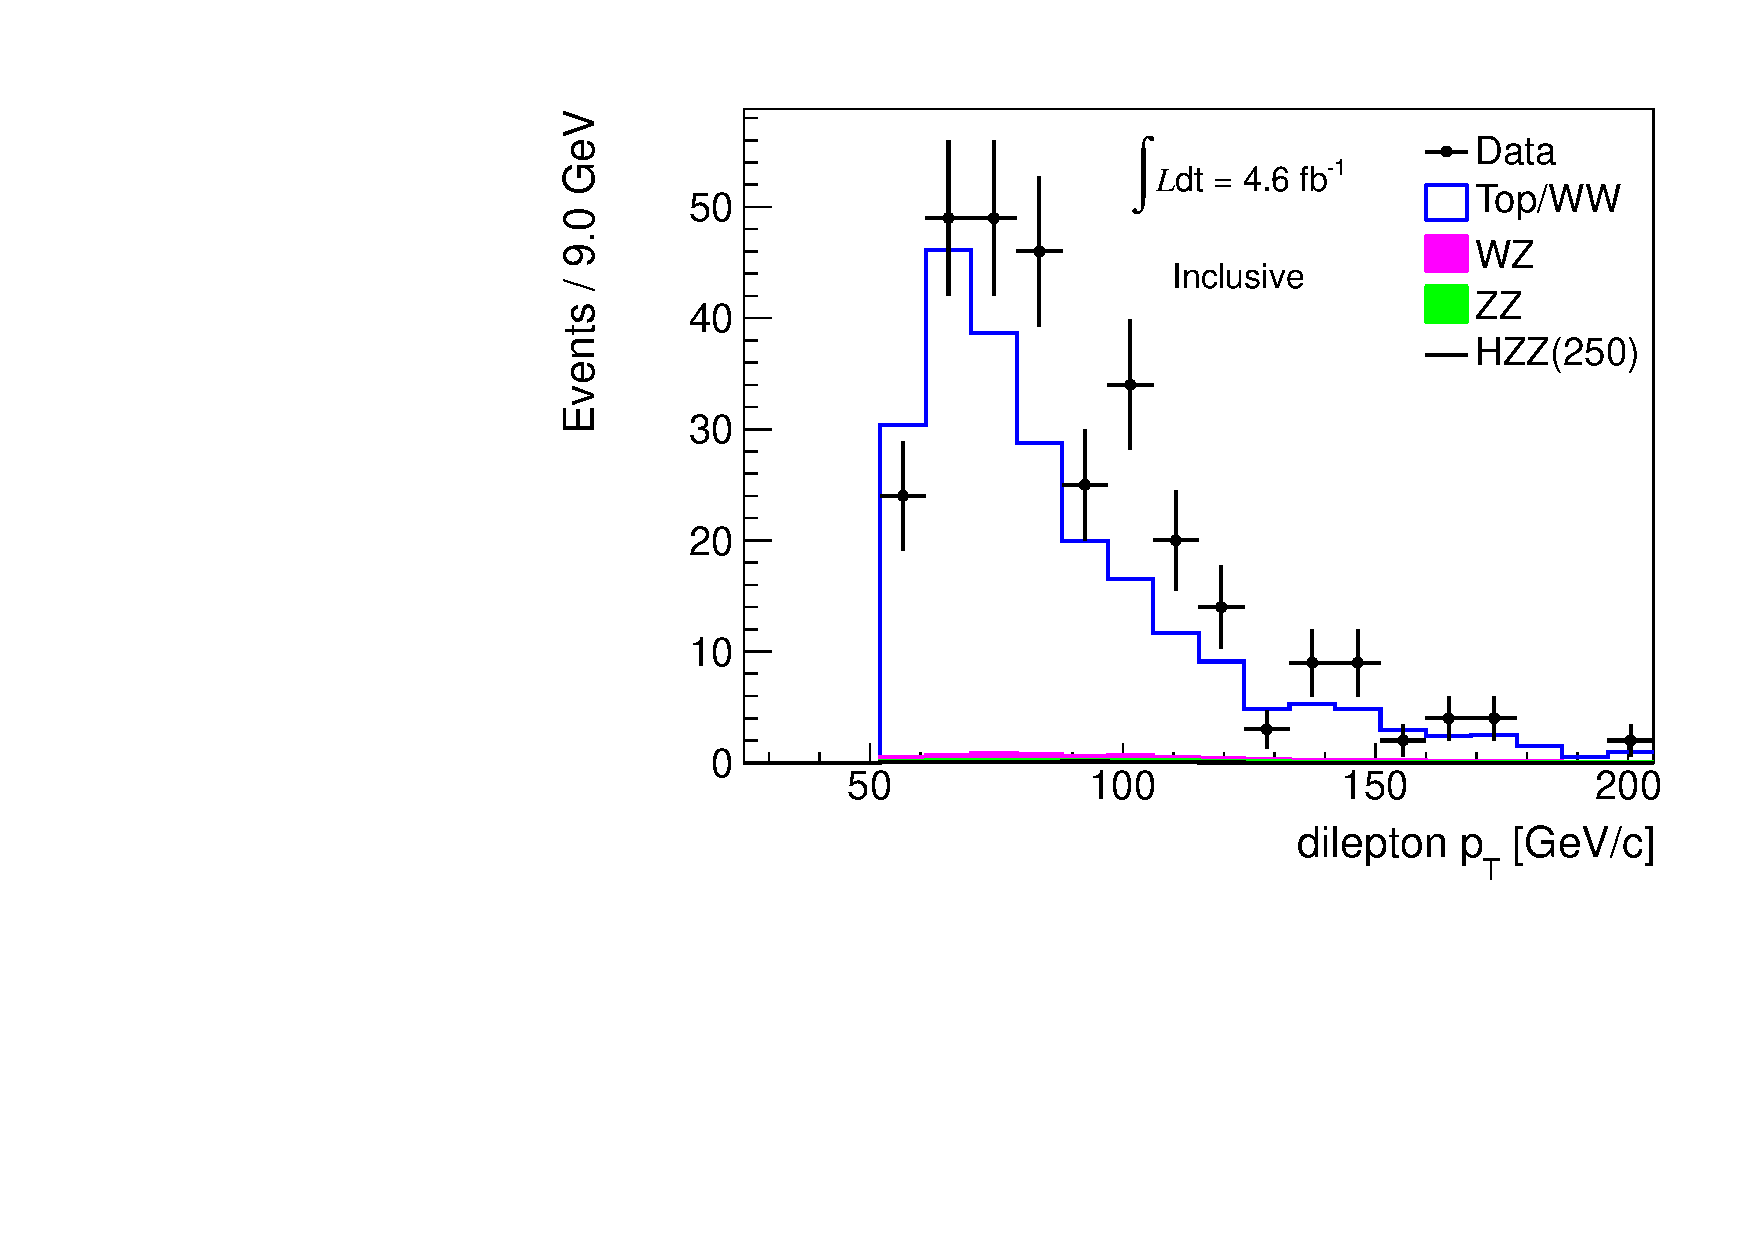
\includegraphics[width=.4\textwidth]{figures/topww_mH250_ee_dileppt_incl.pdf}}
\caption{Distribution for the dilepton $p_T$ in the top/$WW$ control region corresponding 
to $4.0$~\ifb of data in the muon~\subref{subfig:npv_mm} and electron~\subref{subfig:npv_ee} channels, 
compared to the expected from simulation for signal and background. The MC backgrounds are scaled as 
appropriate and the opposite flavor dilepton estimate of the top and $WW$ background is added to the stack.}
\label{fig:topww_dileppt}
\end{center}
\end{figure}
%%%%%%%%

%%%%%%%%
\begin{figure}[!hbtp]
\begin{center}
\subfigure[Inclusive]{\label{subfig:topww_metlog_mm}
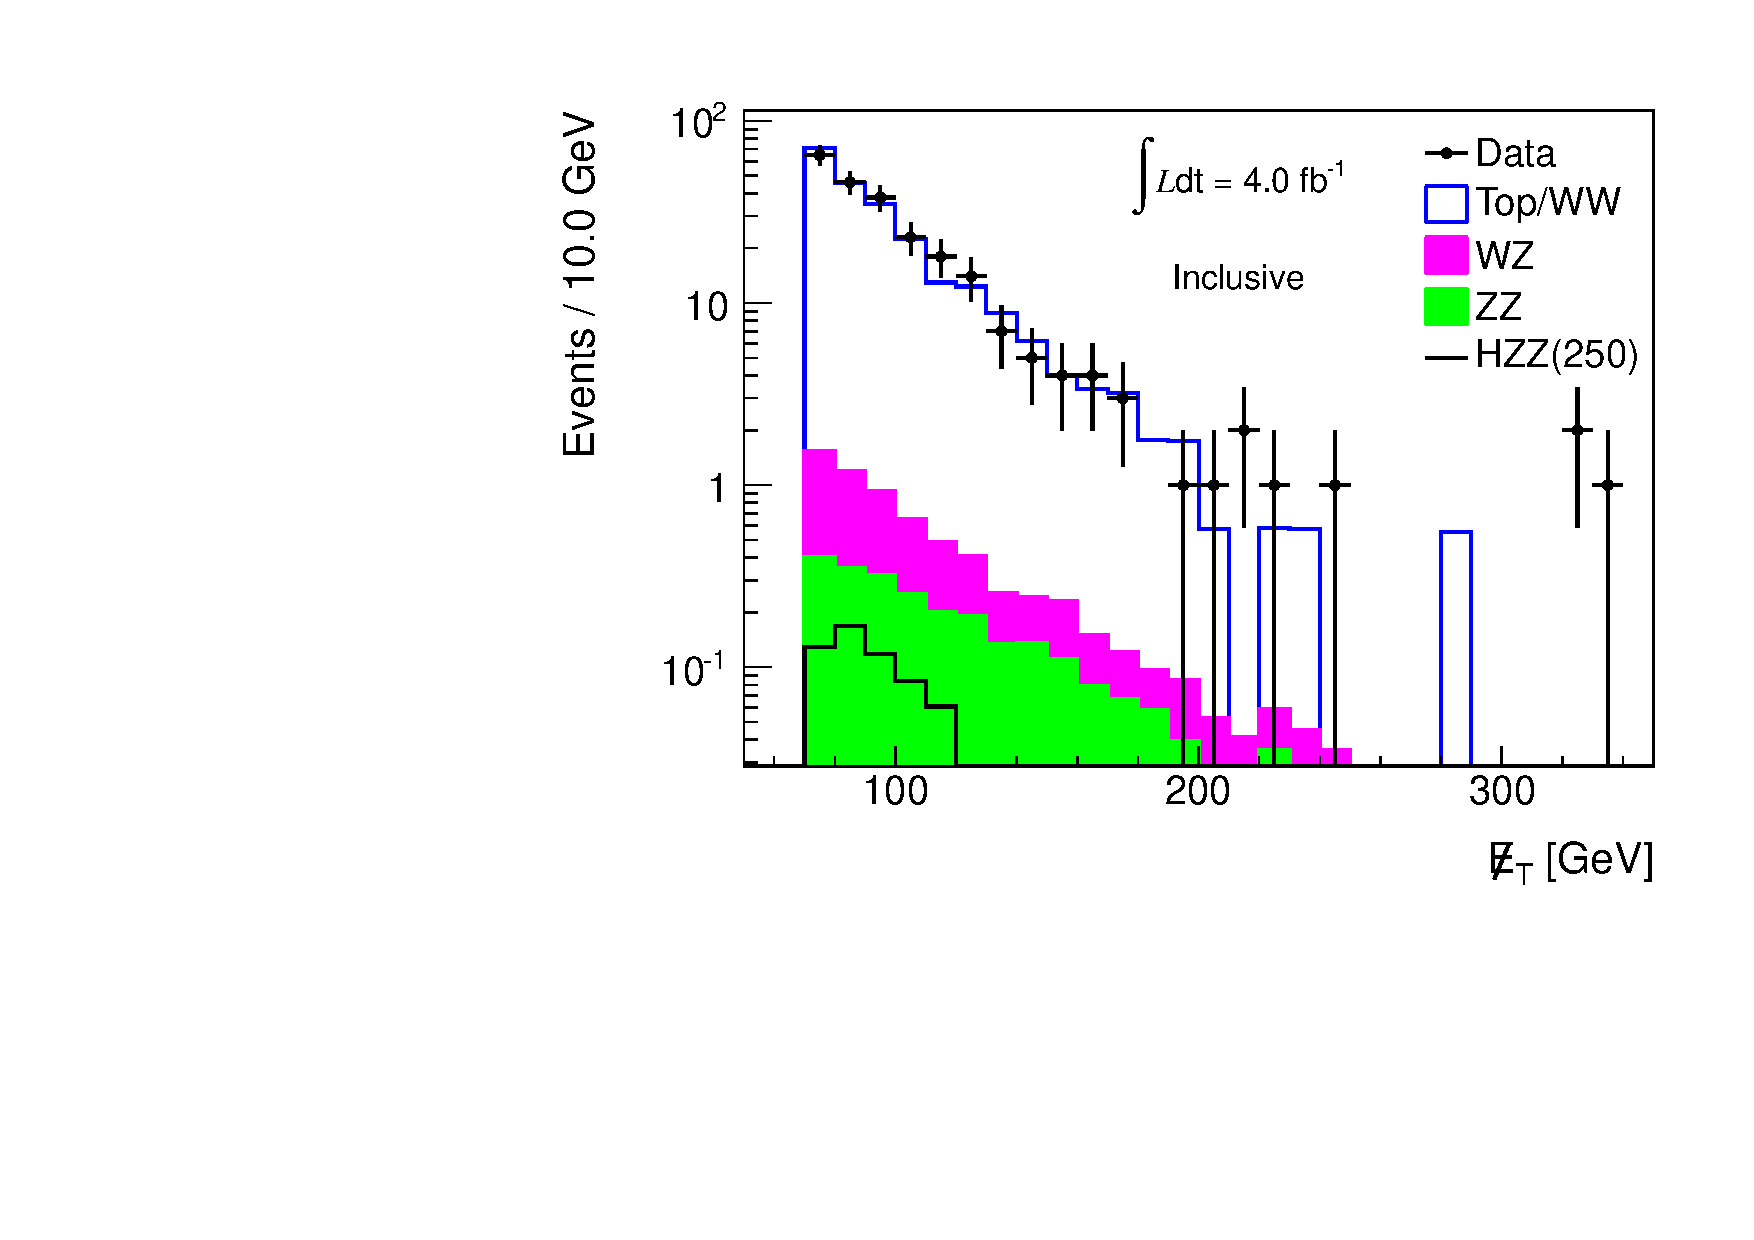
\includegraphics[width=.4\textwidth]{figures/topww_mH250_mm_metlog_incl.pdf}}
\subfigure[1-Jet]{\label{subfig:topww_metlog_ee}
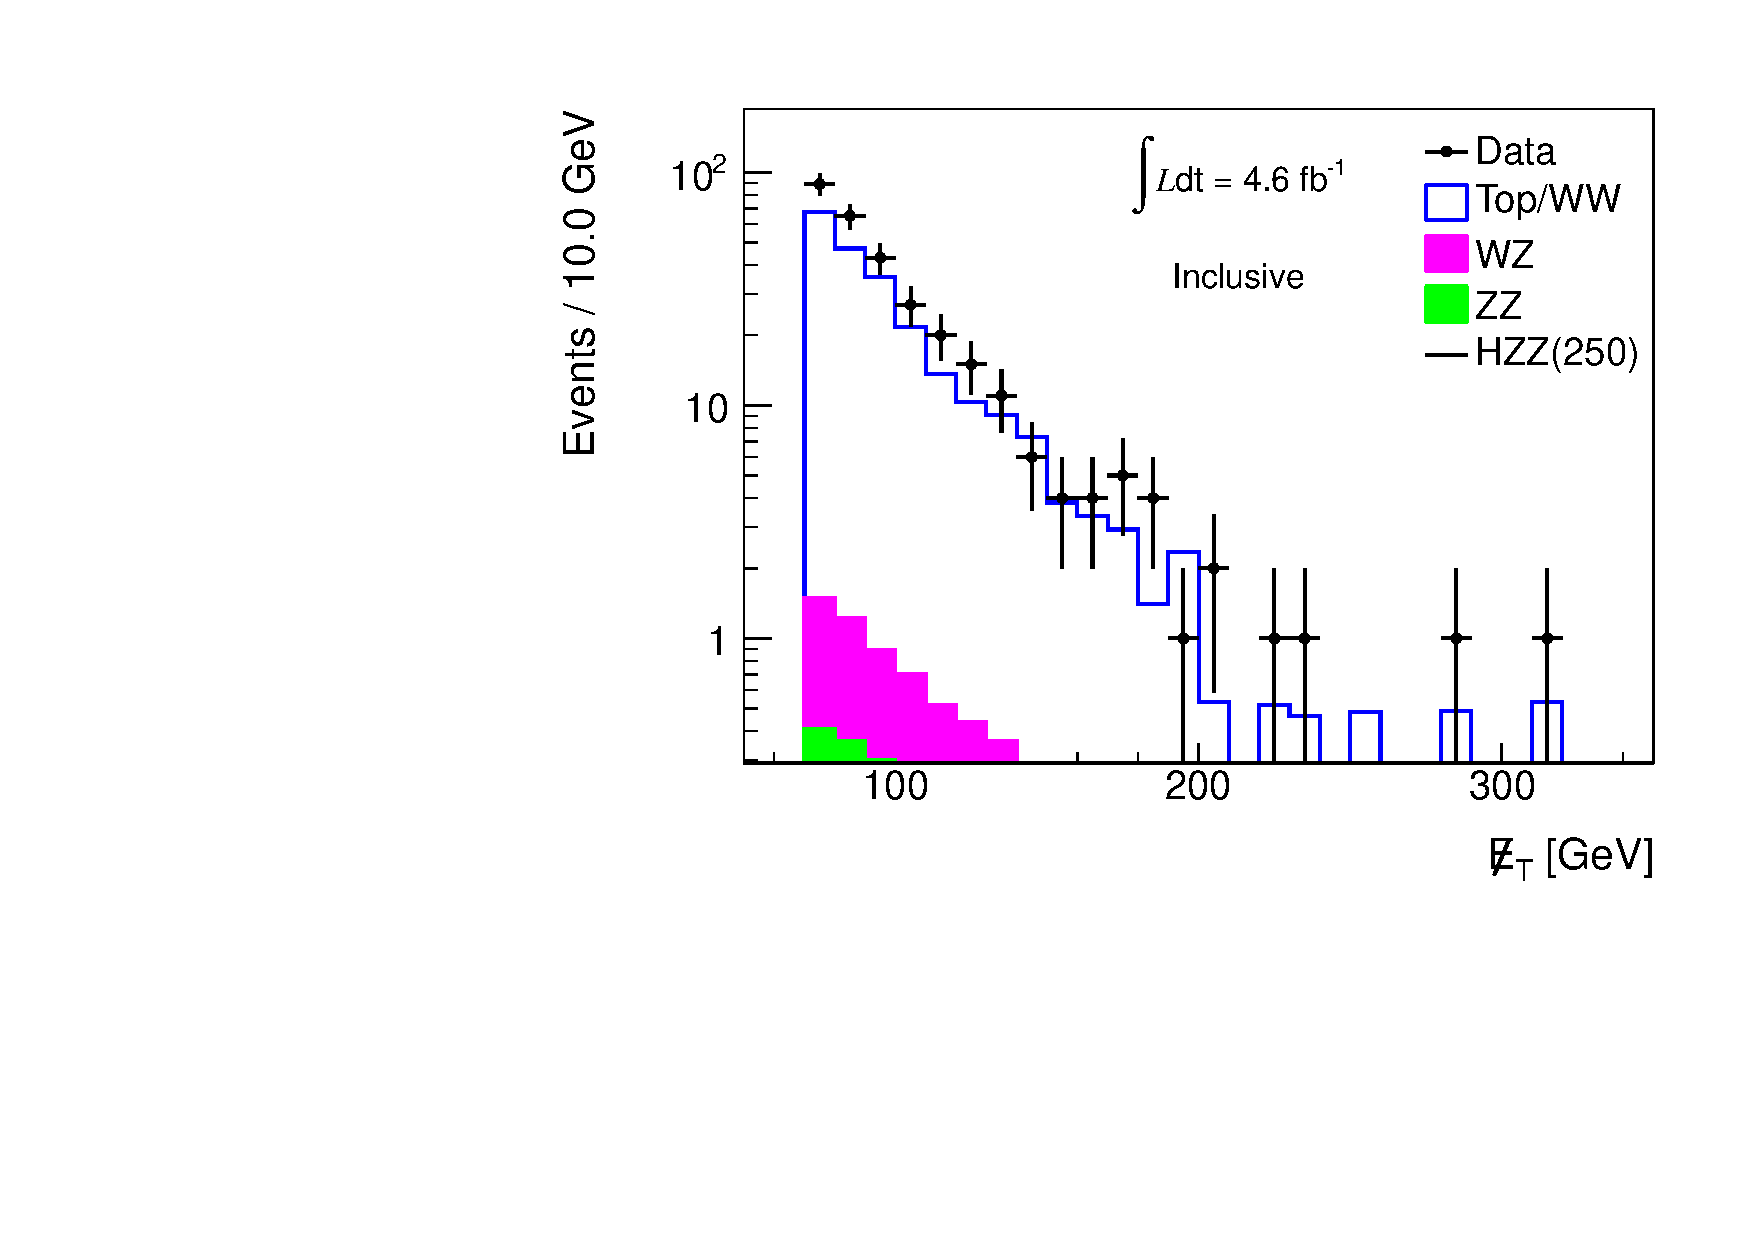
\includegraphics[width=.4\textwidth]{figures/topww_mH250_ee_metlog_incl.pdf}}
\caption{Distribution for the MET in the top/$WW$ control region corresponding 
to $4.0$~\ifb of data in the muon~\subref{subfig:npv_mm} and electron~\subref{subfig:npv_ee} channels, 
compared to the expected from simulation for signal and background. The MC backgrounds are scaled as 
appropriate and the opposite flavor dilepton estimate of the top and $WW$ background is added to the stack.}
\label{fig:topww_metlog}
\end{center}
\end{figure}
%%%%%%%%

%%%%%%%%
\begin{figure}[!hbtp]
\begin{center}
\subfigure[Inclusive]{\label{subfig:topww_mt_mm}
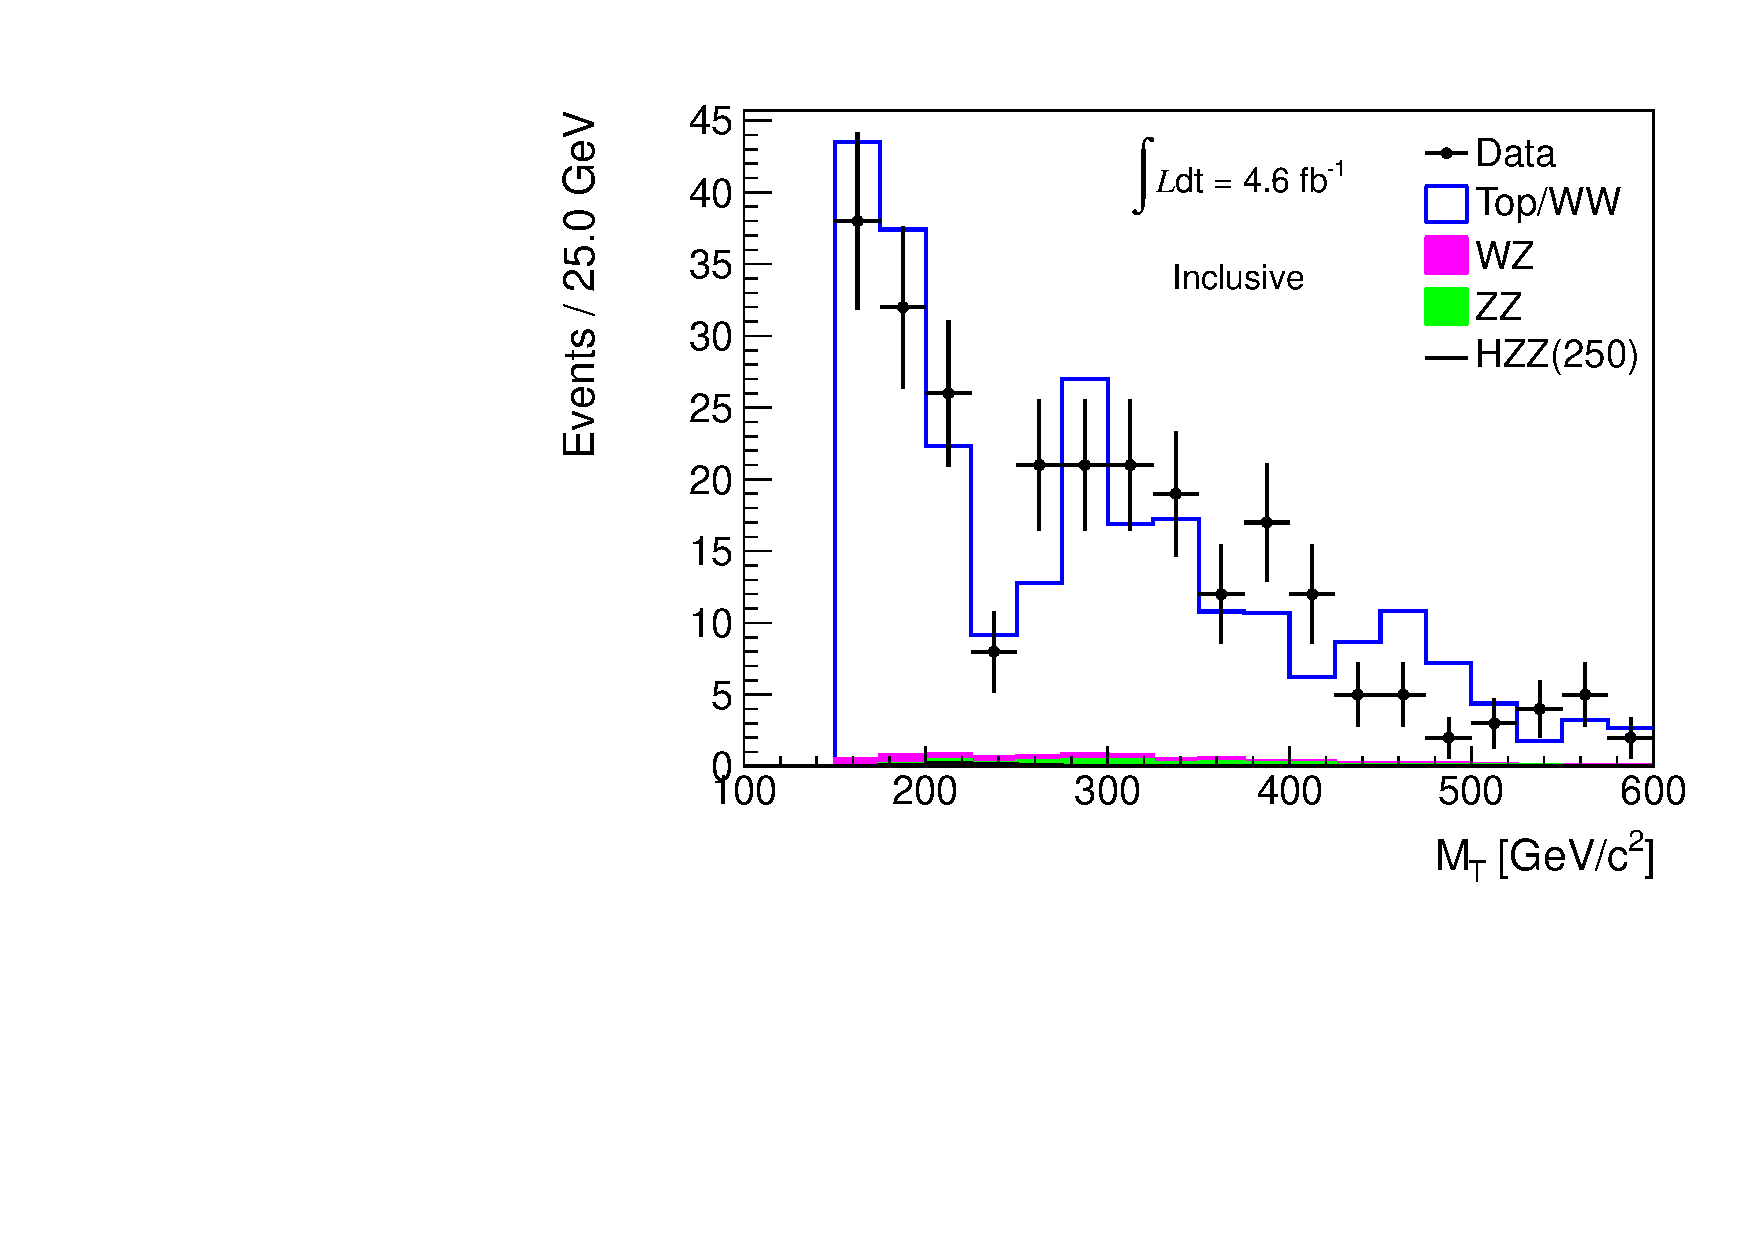
\includegraphics[width=.4\textwidth]{figures/topww_mH250_mm_mt_incl.pdf}}
\subfigure[1-Jet]{\label{subfig:topww_mt_ee}
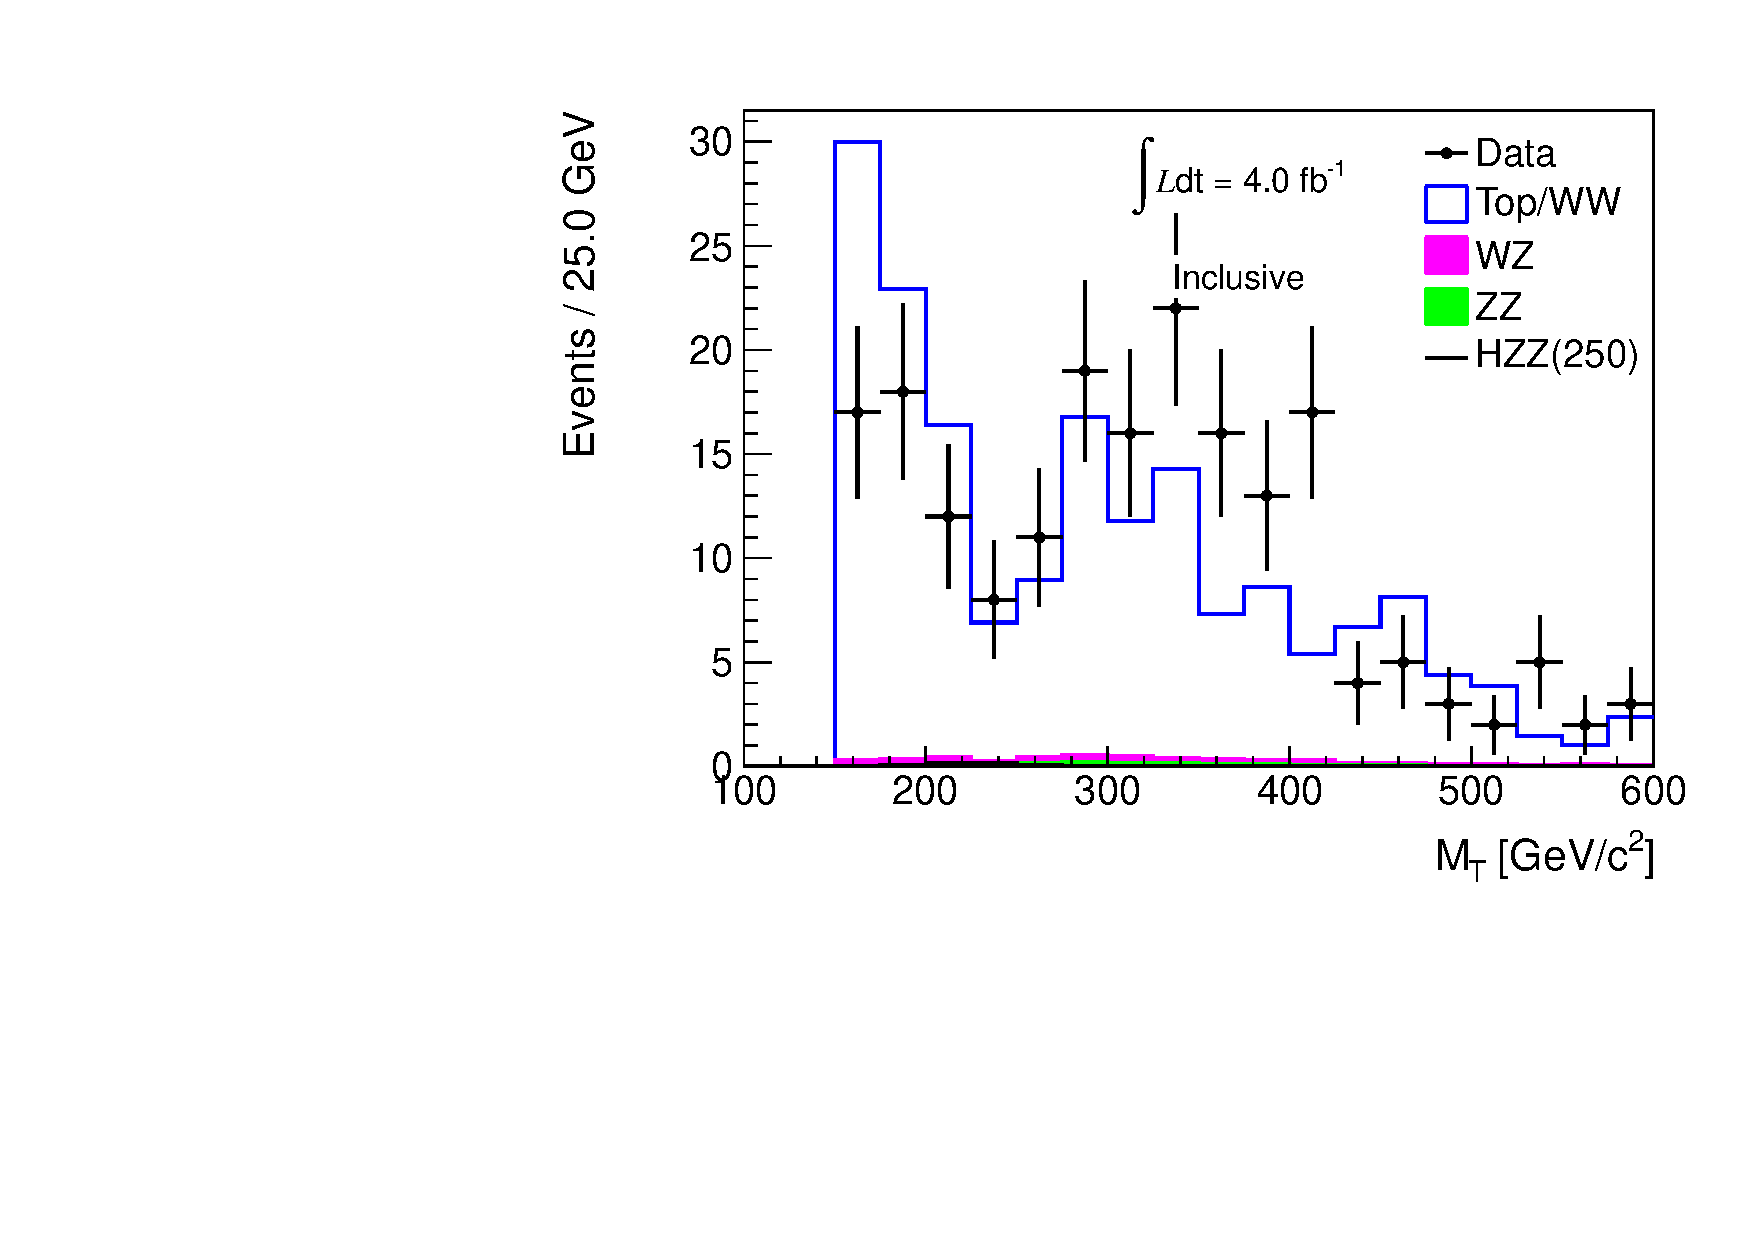
\includegraphics[width=.4\textwidth]{figures/topww_mH250_ee_mt_incl.pdf}}
\caption{Distribution for the dilepton mt in the top/$WW$ control region corresponding 
to $4.0$~\ifb of data in the muon~\subref{subfig:npv_mm} and electron~\subref{subfig:npv_ee} channels, 
compared to the expected from simulation for signal and background. The MC backgrounds are scaled as 
appropriate and the opposite flavor dilepton estimate of the top and $WW$ background is added to the stack.}
\label{fig:topww_mt}
\end{center}
\end{figure}
%%%%%%%%

%%%%%%%%
\begin{figure}[!hbtp]
\begin{center}
\subfigure[Inclusive]{\label{subfig:topww_dphijetmet_mm}
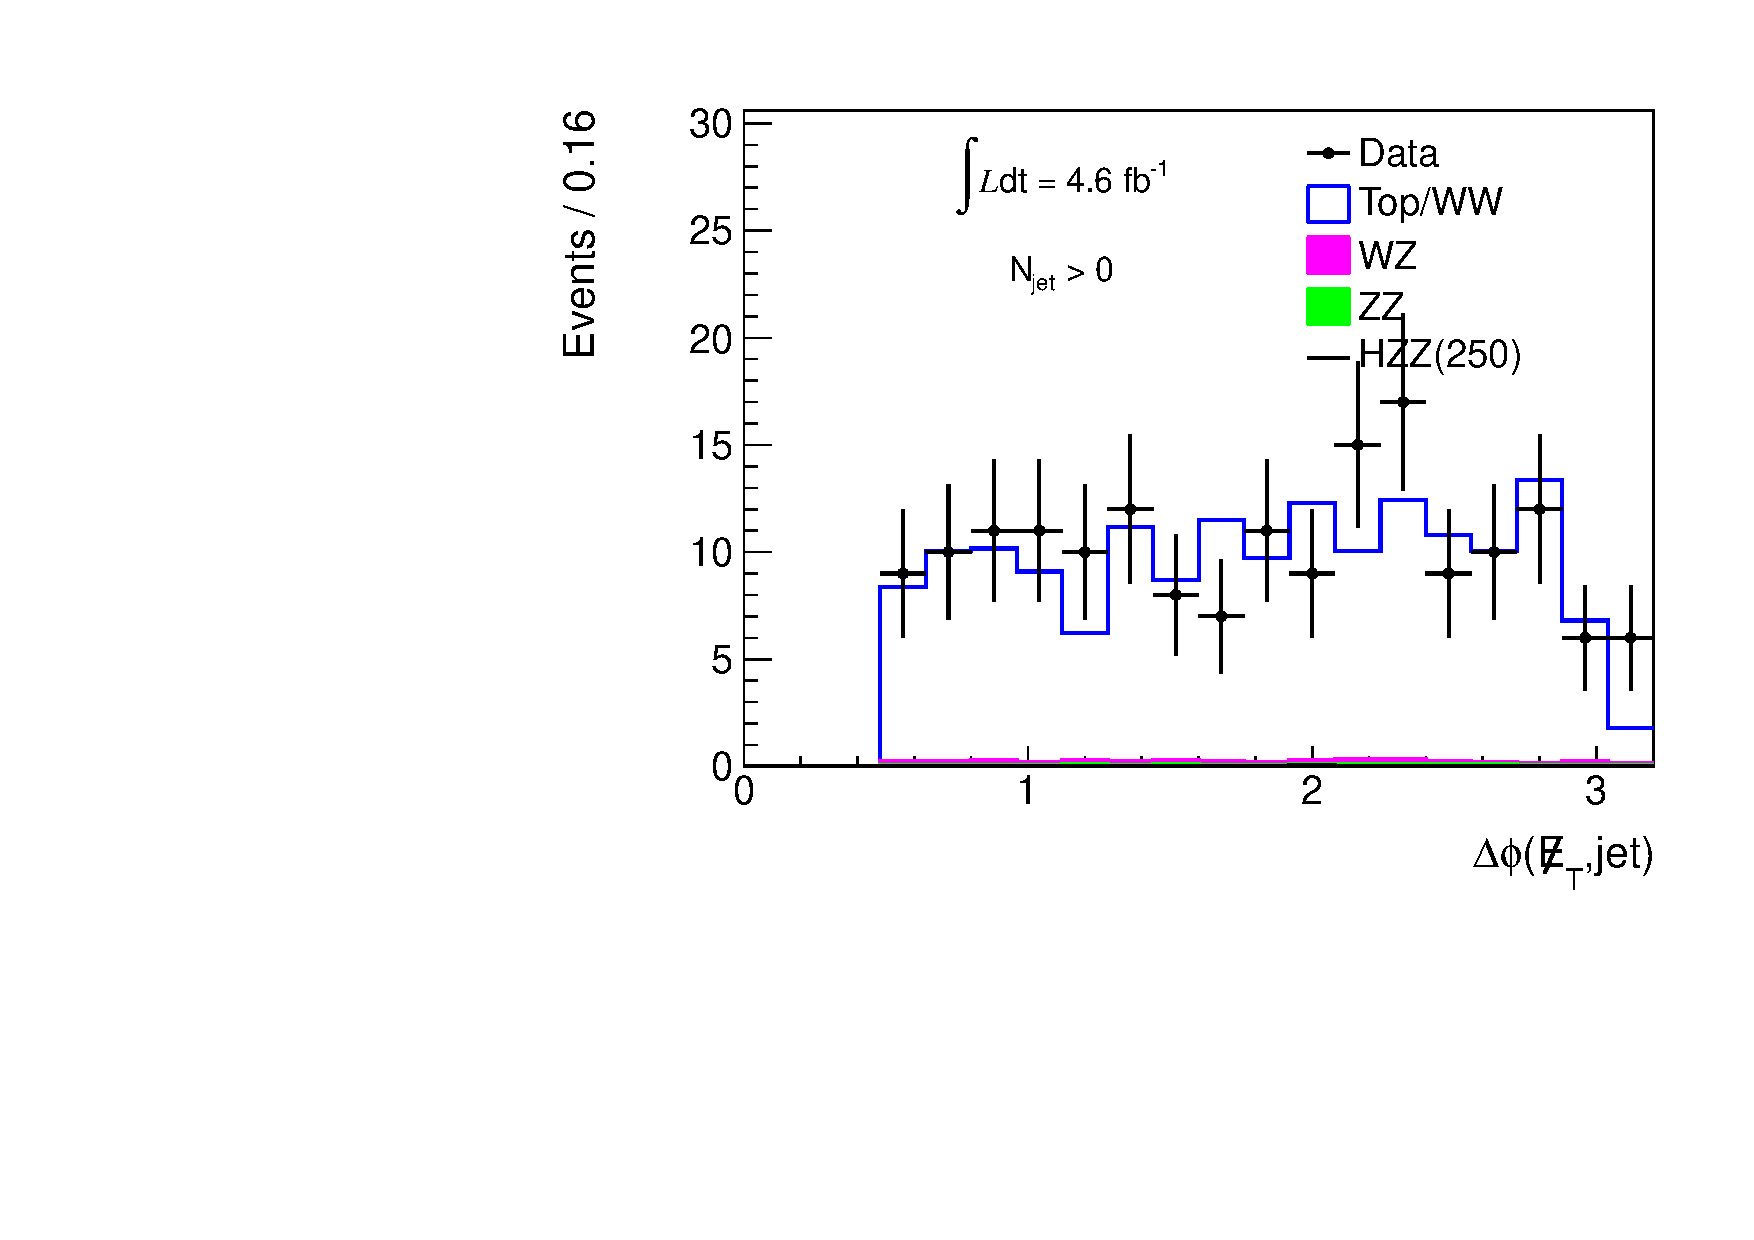
\includegraphics[width=.4\textwidth]{figures/topww_mH250_mm_dphijetmet_incl.pdf}}
\subfigure[1-Jet]{\label{subfig:topww_dphijetmet_ee}
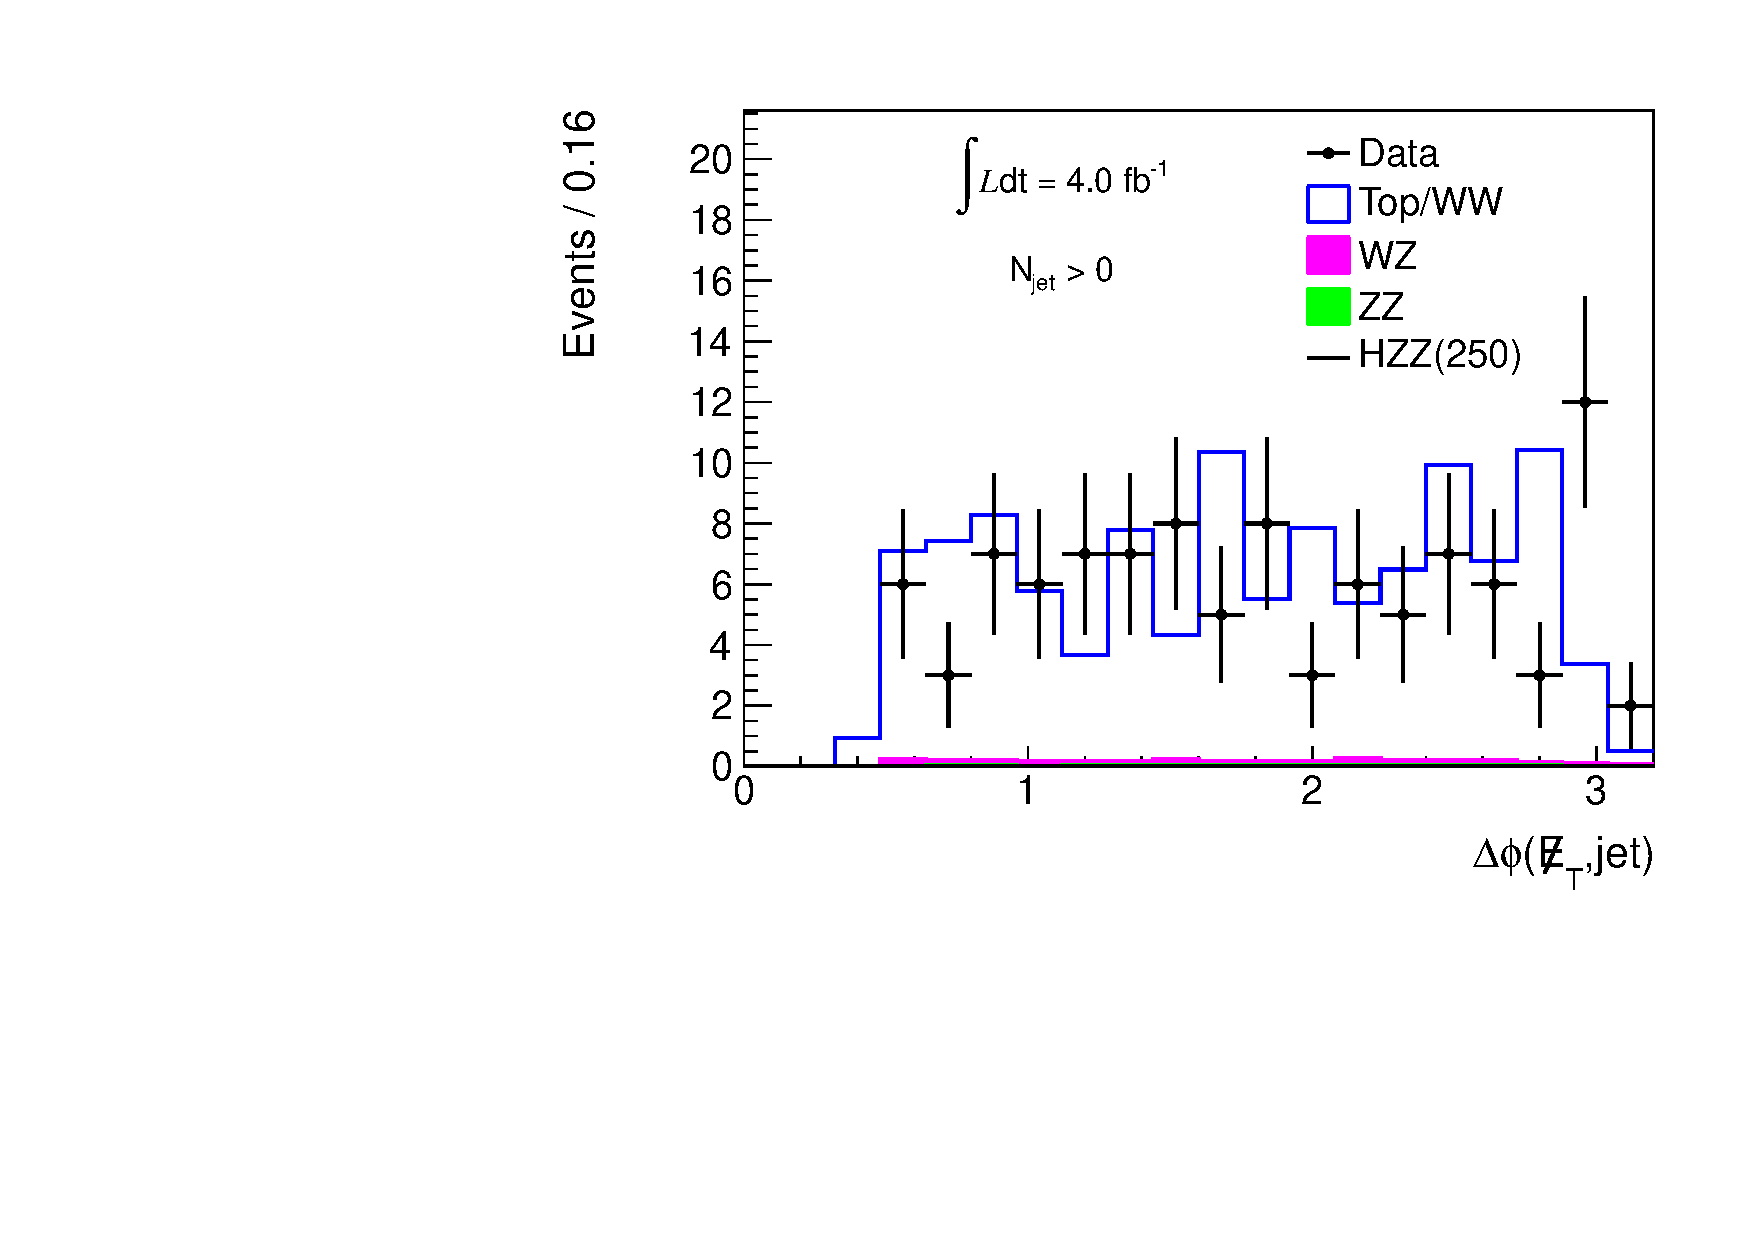
\includegraphics[width=.4\textwidth]{figures/topww_mH250_ee_dphijetmet_incl.pdf}}
\caption{Distribution for the dilepton $\Delta\phi\left(\mbox{jet},\mbox{MET}\right)$ in the top/$WW$ control region corresponding 
to $4.0$~\ifb of data in the muon~\subref{subfig:npv_mm} and electron~\subref{subfig:npv_ee} channels, 
compared to the expected from simulation for signal and background. The MC backgrounds are scaled as 
appropriate and the opposite flavor dilepton estimate of the top and $WW$ background is added to the stack.}
\label{fig:topww_dphijetmet}
\end{center}
\end{figure}
%%%%%%%%

\clearpage

\subsection{Final Results for the Higgs Search with $4.6~\ifb$  }
\label{sec:results_5fb}
In this section we document the results corresponding to \intlumi data, for 
cut-based analysis and the shape based analyses based on both 
$M_T$ variable and the matrix element output. 

Tables~\ref{tab:yield_cutbased}-\ref{tab:yield_me_shapebased} shows the observed number of events and the 
signal and background expectations for the cut-based analysis and shape analysis based on $M_T$ variable 
and matrix element output. The Higgs boson mass dependent signal selections are described in 
Section~\ref{sec:signal_selection}. Note that for the $\dyll$ background the mean value of the 
contribution is the half of the photon jets prediction, without subtracting the contaminations. 
As discussed in Section~\ref{sec:bkg_dy}, 100\% uncertainty is assigned in this case to 
cover the entire range between 0 and the photon jets prediction, which represents the upper-bound of the 
photon jet contribution with $\met$ due to the jet mismeasurement. 

The observed and expected cross section ratio limits as a function of the Higgs mass, together with the 1/2-$\sigma$ uncertainty bands 
are shown in Table~\ref{tab:limits_5fb} and Figure~\ref{fig:limits_5fb} for these three analyses. 
The corresponding $M_T$ and matrix element output distributions are shown in Appendix~\ref{app:mtshape} and Appendix~\ref{app:meshape} respectively.

With the current data sample, we expect to exclude the standard model Higgs boson 
in the mass range of about [300,450]~\GeVcc in the cut-based analysis, compared with the 
expected exclusion range of [300,475]~\GeVcc. 
The observed exclusion region extends to about [275-455]~\GeVcc using shape analysis based on 
$M_T$ variable, compared to the expected exclusion range of [290-490]~\GeVcc.
The observed exclusion region extends to about [300-500]~\GeVcc using shape analysis based on 
matrix element output, compared to the expected exclusion range of [280-480]~\GeVcc.


%%%%%%%%%%%%%%%%%%%%%%%%%
\begin{table}[!htbp]
{\scriptsize
\begin{center}
 \begin{tabular}{l | c c |  c c c c c c | c }
 \hline\hline
 $m_H$ & qqH & ggH & qqZZ & ggZZ & WZ & WWTop & Zjets & $\sum$Bkg & Data \\
 \hline
\multicolumn{10}{c} {ee} \\ \hline
250 & $0.9\pm0.1$ & $8.2\pm1.2$ & $13.2\pm1.4$ & $1.2\pm0.3$ & $9.7\pm1.2$ & $29.4\pm3.6$ & $6.0\pm6.0$ & $59.5\pm6.3$ & 58 \\
300 & $0.9\pm0.1$ & $7.9\pm1.2$ & $8.7\pm0.9$ & $0.8\pm0.2$ & $5.3\pm0.7$ & $9.6\pm2.1$ & $3.0\pm3.0$ & $27.3\pm3.2$ & 20 \\
350 & $0.7\pm0.1$ & $8.0\pm1.3$ & $6.2\pm0.7$ & $0.5\pm0.1$ & $2.8\pm0.4$ & $0.9\pm0.7$ & $1.7\pm1.7$ & $12.2\pm1.9$ & 10 \\
400 & $0.5\pm0.1$ & $6.7\pm1.2$ & $4.6\pm0.5$ & $0.4\pm0.1$ & $1.9\pm0.3$ & $0.0\pm0.4$ & $1.0\pm1.0$ & $8.0\pm1.2$ & 7 \\
500 & $0.3\pm0.1$ & $2.9\pm0.7$ & $2.8\pm0.3$ & $0.2\pm0.0$ & $0.9\pm0.1$ & $0.0\pm0.4$ & $0.5\pm0.5$ & $4.4\pm0.6$ & 5 \\
600 & $0.2\pm0.1$ & $1.1\pm0.4$ & $1.4\pm0.2$ & $0.1\pm0.0$ & $0.4\pm0.1$ & $0.0\pm0.4$ & $0.3\pm0.3$ & $2.2\pm0.3$ & 0 \\
\hline
\multicolumn{10}{c} {$\mu\mu$} \\ 
\hline
250 & $1.3\pm0.1$ & $11.7\pm1.7$ & $19.6\pm1.9$ & $1.8\pm0.4$ & $14.4\pm1.7$ & $36.5\pm4.5$ & $8.6\pm8.6$ & $81.0\pm9.0$ & 82 \\
300 & $1.2\pm0.1$ & $11.2\pm1.6$ & $12.7\pm1.2$ & $1.1\pm0.2$ & $7.5\pm0.9$ & $11.7\pm2.5$ & $4.4\pm4.4$ & $37.4\pm4.6$ & 41 \\
350 & $1.0\pm0.1$ & $11.0\pm1.7$ & $8.5\pm0.8$ & $0.7\pm0.2$ & $4.3\pm0.5$ & $1.1\pm0.7$ & $2.6\pm2.6$ & $17.2\pm2.8$ & 17 \\
400 & $0.7\pm0.1$ & $9.4\pm1.6$ & $6.6\pm0.7$ & $0.5\pm0.1$ & $2.8\pm0.3$ & $0.0\pm0.4$ & $1.6\pm1.6$ & $11.6\pm1.8$ & 11 \\
500 & $0.4\pm0.1$ & $3.9\pm0.9$ & $4.2\pm0.4$ & $0.3\pm0.1$ & $1.2\pm0.2$ & $0.0\pm0.4$ & $0.8\pm0.8$ & $6.5\pm0.9$ & 9 \\
600 & $0.2\pm0.1$ & $1.5\pm0.5$ & $2.2\pm0.2$ & $0.2\pm0.0$ & $0.5\pm0.1$ & $0.0\pm0.4$ & $0.3\pm0.3$ & $3.2\pm0.4$ & 5 \\
\hline\hline
\end{tabular}
\end{center}
}
\caption{Number of events observed in data and the expected signal and background yields 
	for an integrated luminosity of \intlumi 
	after applying the higgs selections in the {\bf cut-based analysis}.}	
%	For the sum of the $\ww$ and Top backgrounds, the uncertainties are modelled by a Gamma function of the number 
%	of $e\mu$ events in the control region.  }
\label{tab:yield_cutbased}
\end{table}
%%%%%%%%%%%%%%%%%%%%%%%%%%%%%%%

%%%%%%%%%%%%%%%%%%%%%%%%%
\begin{table}[!htbp]
{\scriptsize
 \begin{center}
 \begin{tabular}{l | c c | c c c c c c  | c}
 \hline\hline
 $mH$ & qqH & ggH & ZZ & ggZZ & WZ & WW/Top & Zjets & $\sum$Bkg & Data \\
 \hline
\multicolumn{10}{c} {ee} \\ 
\hline
250 & $1.0\pm0.1$ & $8.7\pm1.3$ & $18.0\pm1.9$ & $1.7\pm0.4$ & $14.4\pm1.8$ & $49.3\pm4.7$ & $14.5\pm14.5$ & $97.9\pm15.5$ & 95 \\
300 & $1.0\pm0.1$ & $9.1\pm1.4$ & $12.9\pm1.4$ & $1.1\pm0.3$ & $7.8\pm1.0$ & $17.0\pm2.8$ & $4.4\pm4.4$ & $43.2\pm5.5$ & 32 \\
350 & $1.0\pm0.1$ & $10.4\pm1.7$ & $14.9\pm1.6$ & $1.3\pm0.3$ & $8.7\pm1.1$ & $17.0\pm2.8$ & $5.0\pm5.0$ & $46.8\pm6.0$ & 35 \\
400 & $0.7\pm0.1$ & $8.8\pm1.5$ & $15.9\pm1.7$ & $1.4\pm0.3$ & $9.1\pm1.2$ & $17.0\pm2.8$ & $5.2\pm5.2$ & $48.5\pm6.2$ & 39 \\
500 & $0.4\pm0.1$ & $4.0\pm1.0$ & $17.0\pm1.8$ & $1.5\pm0.3$ & $9.4\pm1.2$ & $17.0\pm2.8$ & $5.4\pm5.4$ & $50.3\pm6.5$ & 39 \\
600 & $0.3\pm0.1$ & $1.7\pm0.6$ & $17.3\pm1.8$ & $1.5\pm0.3$ & $9.5\pm1.2$ & $17.0\pm2.8$ & $5.4\pm5.4$ & $50.8\pm6.5$ & 39 \\
\hline
\multicolumn{10}{c} {$\mu\mu$} \\ 
\hline
250 & $1.5\pm0.1$ & $12.4\pm1.8$ & $26.9\pm2.6$ & $2.5\pm0.5$ & $21.4\pm2.5$ & $61.5\pm5.8$ & $21.7\pm21.7$ & $133.9\pm22.8$ & 140 \\
300 & $1.4\pm0.1$ & $12.9\pm1.9$ & $18.8\pm1.8$ & $1.7\pm0.4$ & $11.2\pm1.3$ & $21.2\pm3.4$ & $7.0\pm7.0$ & $59.9\pm8.2$ & 60 \\
350 & $1.3\pm0.1$ & $14.8\pm2.3$ & $21.5\pm2.1$ & $1.9\pm0.4$ & $12.5\pm1.5$ & $21.2\pm3.4$ & $7.9\pm7.9$ & $65.0\pm9.0$ & 62 \\
400 & $1.0\pm0.1$ & $12.6\pm2.2$ & $23.1\pm2.3$ & $2.0\pm0.4$ & $13.1\pm1.5$ & $21.2\pm3.4$ & $8.2\pm8.2$ & $67.6\pm9.3$ & 65 \\
500 & $0.6\pm0.1$ & $5.5\pm1.3$ & $24.9\pm2.4$ & $2.2\pm0.5$ & $13.5\pm1.6$ & $21.2\pm3.4$ & $8.5\pm8.5$ & $70.2\pm9.6$ & 70 \\
600 & $0.3\pm0.1$ & $2.3\pm0.8$ & $25.3\pm2.5$ & $2.2\pm0.5$ & $13.6\pm1.6$ & $21.2\pm3.4$ & $8.6\pm8.6$ & $70.8\pm9.7$ & 70 \\
\hline\hline
\end{tabular}
\end{center}
}
\caption{Number of events observed in data and the expected signal and background yields for 
	an integrated luminosity of \intlumi after applying the higgs selections in the 
	{\bf shape analysis based on $M_T$}. }
\label{tab:yield_mt_shapebased}
\end{table}
%%%%%%%%%%%%%%%%%%%%%%%%%%%%%%%

%%%%%%%%%%%%%%%%%%%%%%%%%
\begin{table}[!htbp]
{\scriptsize
 \begin{center}
 \begin{tabular}{l | c c | c c c c c c | c}
 \hline\hline
 $mH$ & qqH & ggH & ZZ & ggZZ & WZ & WW/Top & Zjets & $\sum$Bkg & Data \\
 \hline
\multicolumn{10}{c} {ee} \\ 
\hline
250 & $1.1\pm0.1$ & $8.9\pm1.3$ & $27.4\pm2.9$ & $2.4\pm0.5$ & $18.7\pm2.3$ & $54.7\pm4.9$ & $18.9\pm18.9$ & $122.1\pm19.9$ & 115 \\
300 & $1.2\pm0.1$ & $10.3\pm1.6$ & $22.4\pm2.4$ & $2.0\pm0.4$ & $14.3\pm1.8$ & $38.9\pm4.2$ & $11.5\pm11.5$ & $89.1\pm12.6$ & 84 \\
350 & $1.0\pm0.1$ & $10.8\pm1.7$ & $18.2\pm1.9$ & $1.6\pm0.4$ & $10.6\pm1.3$ & $22.6\pm3.2$ & $8.1\pm8.1$ & $61.2\pm9.0$ & 58 \\
400 & $0.7\pm0.1$ & $9.3\pm1.6$ & $18.2\pm1.9$ & $1.6\pm0.4$ & $10.6\pm1.3$ & $22.6\pm3.2$ & $8.1\pm8.1$ & $61.2\pm9.0$ & 58 \\
500 & $0.4\pm0.1$ & $4.2\pm1.0$ & $14.8\pm1.6$ & $1.3\pm0.3$ & $8.0\pm1.0$ & $14.3\pm2.5$ & $5.9\pm5.9$ & $44.3\pm6.7$ & 47 \\
600 & $0.2\pm0.1$ & $1.6\pm0.6$ & $9.9\pm1.0$ & $0.8\pm0.2$ & $4.6\pm0.6$ & $3.6\pm1.3$ & $3.4\pm3.4$ & $22.4\pm3.9$ & 26 \\
\hline
\multicolumn{10}{c} {$\mu\mu$} \\ 
\hline
250 & $1.5\pm0.1$ & $12.8\pm1.8$ & $40.3\pm3.9$ & $3.6\pm0.8$ & $27.6\pm3.2$ & $68.1\pm6.1$ & $27.9\pm27.9$ & $167.5\pm29.1$ & 173 \\
300 & $1.7\pm0.1$ & $14.8\pm2.2$ & $33.2\pm3.2$ & $2.9\pm0.6$ & $20.8\pm2.4$ & $48.1\pm5.2$ & $17.1\pm17.1$ & $122.1\pm18.3$ & 125 \\
350 & $1.4\pm0.1$ & $15.3\pm2.4$ & $26.8\pm2.6$ & $2.3\pm0.5$ & $15.6\pm1.8$ & $28.2\pm3.9$ & $12.0\pm12.0$ & $85.0\pm13.1$ & 89 \\
400 & $1.0\pm0.1$ & $13.3\pm2.3$ & $26.8\pm2.6$ & $2.3\pm0.5$ & $15.6\pm1.8$ & $28.2\pm3.9$ & $12.0\pm12.0$ & $85.0\pm13.1$ & 89 \\
500 & $0.6\pm0.1$ & $5.6\pm1.3$ & $21.6\pm2.1$ & $1.8\pm0.4$ & $11.8\pm1.4$ & $17.8\pm3.2$ & $8.8\pm8.8$ & $61.8\pm9.7$ & 63 \\
600 & $0.3\pm0.1$ & $2.3\pm0.8$ & $14.2\pm1.4$ & $1.2\pm0.3$ & $6.7\pm0.8$ & $4.5\pm1.6$ & $5.0\pm5.0$ & $31.7\pm5.5$ & 34 \\
\hline\hline
\end{tabular}
\end{center}
}
\caption{Number of events observed in data and the expected signal and background yields for an integrated 
	luminosity of \intlumi 	after applying the higgs selections in the 
	{\bf shape analysis based on matrix element output}. }
\label{tab:yield_me_shapebased}
\end{table}
%%%%%%%%%%%%%%%%%%%%%%%

%%%%%%%%%%%%%%%%%%%%%%%%%%%%%%%
\begin{table}[!htbp]
\begin{center}
\begin{tabular}{ccccc}
\hline\hline
Mass & Observed & Median Expected & [-$\sigma$, +$\sigma$] & [-2$\sigma$, +2$\sigma$]\\\hline
\hline
\multicolumn{5}{c} {Cut-based Analysis} \\ 
\hline
250 & 1.62 & 1.62 & [1.17, 2.24] & [0.88, 2.98] \\
300 & 0.95 & 1.04 & [0.75, 1.44] & [0.56, 1.91] \\
350 & 0.60 & 0.68 & [0.49, 0.94] & [0.37, 1.25] \\
400 & 0.59 & 0.65 & [0.47, 0.91] & [0.35, 1.21] \\
500 & 1.61 & 1.19 & [0.86, 1.66] & [0.65, 2.20] \\
600 & 2.20 & 2.36 & [1.70, 3.28] & [1.28, 4.36] \\
\hline
\multicolumn{5}{c} {Shape Analysis Based on $M_T$} \\ 
\hline
250 & 1.50 & 1.38 & [1.00, 1.92] & [0.75, 2.56] \\
300 & 0.66 & 0.93 & [0.67, 1.29] & [0.51, 1.72] \\
350 & 0.55 & 0.63 & [0.45, 0.87] & [0.34, 1.16] \\
400 & 0.54 & 0.63 & [0.46, 0.88] & [0.34, 1.17] \\
500 & 1.58 & 1.08 & [0.78, 1.50] & [0.58, 1.99] \\
600 & 2.41 & 2.23 & [1.61, 3.10] & [1.21, 4.12] \\
\hline
\multicolumn{5}{c} {Shape Analysis Based on Matrix Element Output} \\ 
\hline
250 & 1.20 & 1.31 & [0.95, 1.83] & [0.71, 2.43] \\
300 & 0.99 & 0.87 & [0.63, 1.21] & [0.47, 1.60] \\
350 & 0.63 & 0.64 & [0.46, 0.88] & [0.35, 1.18] \\
400 & 0.56 & 0.64 & [0.46, 0.89] & [0.35, 1.19] \\
500 & 0.99 & 1.13 & [0.82, 1.57] & [0.61, 2.09] \\
600 & 1.96 & 2.43 & [1.75, 3.37] & [1.32, 4.48] \\
\hline\hline
\end{tabular}
\end{center}
\caption{The observed and expected cross section ratio limits as a function 
of the Higgs mass, together with the 1/2-$\sigma$ uncertainty bands obtained in the cut-and-count analysis 
and shape analyses based on both $M_T$ variable and matrix element output.
The limits correspond to an integrated luminosity of \intlumi, shown in Figure~\ref{fig:limits_5fb}.}
\label{tab:limits_5fb}
\end{table}
%%%%%%%%%%%%%%%%%%%%%%%%%%%%%



%%%%%%%%%%%%%%%%%%%%%%%%%%%%%
\begin{figure}[!htbp]
  \begin{center}
  \subfigure[Cut-based Analysis]{
  \label{subfig:cutbased}
  \includegraphics[width=0.5\textwidth]{figures/limits_cut_5fb.pdf}} \\
\end{center}
  \subfigure[$M_T$ Shape Analysis]{
  \centering
  \label{subfig:mtshape}
   \includegraphics[width=0.5\textwidth]{figures/limits_mtshape_5fb.pdf}}
  \subfigure[Matrix Element Shape Analysis]{
  \centering
  \label{subfig:meshape}
   \includegraphics[width=0.5\textwidth]{figures/limits_meshape_5fb.pdf}}
\caption{The observed and expected upper limits at 95\% C.L. for \intlumi\ of data for the 
	cut-based analysis \subref{subfig:cutbased} and 
	shape analyses based on both $M_T$ variable \subref{subfig:mtshape} 
	and matrix element output \subref{subfig:meshape} The values are 
	tabulated in Table~\ref{tab:limits_5fb}.  
}	
\label{fig:limits_5fb}
\end{figure}
%%%%%%%%%%%%%%%%%%%%%%%%%%%%%


\clearpage

\clearpage

%\subsection{Results in shape analysis based on $M_T$}
%\label{sec:results_mtshape}
%moThe Higgs boson mass dependent signal selections are described in Section~\ref{sec:signal_selection}. 
In this section we summarise the results obtained all jet final states. 
Tables~\ref{tab:yield_mt_shapebased} shows the signal and 
equivalent data yields and background expectations in ee and $\mu\mu$ final states respectively. 
Figure~\ref{fig:histo_mt_250_5fb}-\ref{fig:histo_mt_600_5fb} show the $M_T$ distribution 
after the higgs mass dependent selections, for the mass hypothesis between 250 and 600 $\GeV$, 
corresponding to \intlumi. In these figures the background normalizations are scaled by 
each individual data-to-mc scale factors to account for the data and MC difference in 
background estimation described in section~\ref{sec:backgrounds}, 
lepton efficiency and the pileup reweighting. 

We consider the following uncertainties due to the shape variations, 
%%%%%%%%%%%%%%%%%%%%%%%%%%%%%
\begin{itemize}
\item {Statistic uncertainties in the template}
\item {QCD scale variations to the Higgs process}
\item {Top/WW shape variations}
\item {WZ shape variations}
\item {ZZ shape variations}.
\end{itemize}
%%%%%%%%%%%%%%%%%%%%%%%%%%%%%
The effects due to the lepton efficiency and scale variations are neglible and we assign only 
the normalization uncertainties. 
To understand the effects of the individual source of the uncertainties, 
we also compare the results by adding each source progressively, shown in Table~\ref{tab:mva_mtshape_detail}. 
Among all the shape systematics, the variations of the combined Top/WW shape is the leading effect. 
The details are documented in Ref.~\cite{shapeananote}. 

The expected cross section ratio limits as a function of the Higgs mass, together with the 1/2-$\sigma$ 
uncertainty bands are shown in Table~\ref{tab:limits_mtshape_5fb}. 
Table~\ref{tab:limits_mtshape_5fb} and Figure~\ref{fig:limits_5fb} show the 
observed and expected cross-section ratio limits. 
The observed exclusion region for the Standard Model Higgs is [275,455]~\GeV{} at 95\%C.L., 
compared to the expected exclusion region as [290,490]~\GeV{} at 95\%C.L.
Compared to the cut-based analysis, the shape analysis based on the $M_T$ variable improves the search sensitivity 
by upto $10\%$ considering all the shape variation systematics. 

%%%%%%%%%%%%%%%%%%%%%%%%%
\begin{table}[!ht]
{\scriptsize
 \begin{center}
 \begin{tabular}{l | c c | c c c c c c  | c}
 \hline\hline
 $mH$ & qqH & ggH & ZZ & ggZZ & WZ & WW/Top & Zjets & $\sum$Bkg & Data \\
 \hline
\multicolumn{10}{c} {ee} \\ 
\hline
250 & $1.0\pm0.1$ & $8.7\pm1.3$ & $18.0\pm1.9$ & $1.7\pm0.4$ & $14.4\pm1.8$ & $48.0\pm4.6$ & $14.5\pm14.5$ & $97.1\pm15.5$ & 95 \\
300 & $1.0\pm0.1$ & $9.1\pm1.4$ & $12.9\pm1.4$ & $1.1\pm0.3$ & $7.8\pm1.0$ & $17.0\pm2.8$ & $4.4\pm4.4$ & $43.2\pm5.5$ & 32 \\
350 & $1.0\pm0.1$ & $10.4\pm1.7$ & $14.9\pm1.6$ & $1.3\pm0.3$ & $8.7\pm1.1$ & $17.0\pm2.8$ & $5.0\pm5.0$ & $46.8\pm6.0$ & 35 \\
400 & $0.7\pm0.1$ & $8.8\pm1.5$ & $15.9\pm1.7$ & $1.4\pm0.3$ & $9.1\pm1.2$ & $17.0\pm2.8$ & $5.2\pm5.2$ & $48.5\pm6.2$ & 39 \\
500 & $0.4\pm0.1$ & $4.0\pm1.0$ & $17.0\pm1.8$ & $1.5\pm0.3$ & $9.4\pm1.2$ & $17.0\pm2.8$ & $5.4\pm5.4$ & $50.3\pm6.5$ & 39 \\
600 & $0.3\pm0.1$ & $1.7\pm0.6$ & $17.3\pm1.8$ & $1.5\pm0.3$ & $9.5\pm1.2$ & $17.0\pm2.8$ & $5.4\pm5.4$ & $50.8\pm6.5$ & 39 \\
\hline
\multicolumn{10}{c} {$\mu\mu$} \\ 
\hline
250 & $1.5\pm0.1$ & $12.4\pm1.8$ & $26.9\pm2.6$ & $2.5\pm0.5$ & $21.4\pm2.5$ & $59.8\pm5.7$ & $21.7\pm21.7$ & $132.6\pm22.7$ & 134 \\
300 & $1.4\pm0.1$ & $12.9\pm1.9$ & $18.8\pm1.8$ & $1.7\pm0.4$ & $11.2\pm1.3$ & $21.2\pm3.4$ & $7.0\pm7.0$ & $59.9\pm8.2$ & 60 \\
350 & $1.3\pm0.1$ & $14.8\pm2.3$ & $21.5\pm2.1$ & $1.9\pm0.4$ & $12.5\pm1.5$ & $21.2\pm3.4$ & $7.9\pm7.9$ & $65.0\pm9.0$ & 62 \\
400 & $1.0\pm0.1$ & $12.6\pm2.2$ & $23.1\pm2.3$ & $2.0\pm0.4$ & $13.1\pm1.5$ & $21.2\pm3.4$ & $8.2\pm8.2$ & $67.6\pm9.3$ & 65 \\
500 & $0.6\pm0.1$ & $5.5\pm1.3$ & $24.9\pm2.4$ & $2.2\pm0.5$ & $13.5\pm1.6$ & $21.2\pm3.4$ & $8.5\pm8.5$ & $70.2\pm9.6$ & 70 \\
600 & $0.3\pm0.1$ & $2.3\pm0.8$ & $25.3\pm2.5$ & $2.2\pm0.5$ & $13.6\pm1.6$ & $21.2\pm3.4$ & $8.6\pm8.6$ & $70.8\pm9.7$ & 70 \\
\hline\hline
\end{tabular}
\end{center}
}
\caption{Expected number of signal and background events for an 
  integrated luminosity of \intlumi after applying the higgs selections in the shape-based analysis in the ee final state. 
  Both statistical and systematic uncertainties are included. }
\label{tab:yield_mt_shapebased}
\end{table}



\begin{table}
\begin{center}
{\normalsize
\begin{tabular}{|l|c|c|c|c|c|c|}
\hline
      &  \multicolumn{3}{c|}{ without shape uncertainty} &\multicolumn{3}{c|}{ with shape uncertainty} \\
\hline
Mass  &  Median      &     68\% C.L. band &  95\% C.L. band &  Median	   &	 68\% C.L. band &  95\% C.L. band\\
      &  Expected    &                    &                 &  Expected    &			&		 \\
\hline

250 & 1.36 & [0.98, 1.89] & [0.74, 2.51] & 1.36 & [0.98, 1.89] & [0.74, 2.52] \\
300 & 0.92 & [0.66, 1.27] & [0.50, 1.69] & 0.93 & [0.67, 1.29] & [0.50, 1.72] \\
350 & 0.61 & [0.44, 0.85] & [0.33, 1.13] & 0.62 & [0.45, 0.86] & [0.34, 1.15] \\
400 & 0.62 & [0.45, 0.86] & [0.34, 1.15] & 0.63 & [0.45, 0.87] & [0.34, 1.16] \\
500 & 1.05 & [0.76, 1.46] & [0.57, 1.95] & 1.07 & [0.77, 1.49] & [0.58, 1.98] \\
600 & 2.19 & [1.58, 3.05] & [1.19, 4.05] & 2.22 & [1.60, 3.08] & [1.20, 4.09] \\
\hline
\end{tabular}
}
\end{center}
\caption{The median expected cross section ratio limits as a function 
of the Higgs mass, together with the 1/2-$\sigma$ uncertainty bands obtained in the shape analysis based on $M_T$, 
corresponding to an integrated luminosity of \intlumi}
\label{tab:limits_mtshape_5fb_detail}
\end{table}

%%%%%%%%%%%%%%%%%%%%%%
\begin{figure}[!ht]
\begin{center}
   \subfigure[]{\includegraphics[width=0.4\textwidth,angle=0]{figures/MT_mH250_ee_stack_log.pdf}} 
   \subfigure[]{\includegraphics[width=0.4\textwidth,angle=0]{figures/MT_mH250_mm_stack_log.pdf}} \\ 
   \caption{The $M_T$ distribution for Higgs signal and background events 
for \mHi=250 $\GeVcc$ in ee (a) and $\mu\mu$ final state (b) after the higgs dependent selections. 
The distributions are normalized to \intlumi with the background scaled by the data-to-mc ratios derived from data.}
   \label{fig:histo_mt_250_5fb}
\end{center}
%\end{figure}

%\begin{figure}[!ht]
\begin{center}
   \subfigure[]{\includegraphics[width=0.4\textwidth,angle=0]{figures/MT_mH300_ee_stack_log.pdf}} 
   \subfigure[]{\includegraphics[width=0.4\textwidth,angle=0]{figures/MT_mH300_mm_stack_log.pdf}} \\ 
   \caption{The $M_T$ distribution for Higgs signal and background events 
for \mHi=300 $\GeVcc$ in ee (a) and $\mu\mu$ final state (b) after the higgs dependent selections. 
The distributions are normalized to \intlumi with the background scaled by the data-to-mc ratios derived from data.}
   \label{fig:histo_mt_300_5fb}
\end{center}
%\end{figure}

%\begin{figure}[!ht]
\begin{center}
   \subfigure[]{\includegraphics[width=0.4\textwidth,angle=0]{figures/MT_mH350_ee_stack_log.pdf}} 
   \subfigure[]{\includegraphics[width=0.4\textwidth,angle=0]{figures/MT_mH350_mm_stack_log.pdf}} \\ 
   \caption{The $M_T$ distribution for Higgs signal and background events 
for \mHi=350 $\GeVcc$ in ee (a) and $\mu\mu$ final state (b) after the higgs dependent selections. 
The distributions are normalized to \intlumi with the background scaled by the data-to-mc ratios derived from data.}
   \label{fig:histo_mt_350_5fb}
\end{center}
\end{figure}

\begin{figure}[!ht]
\begin{center}
   \subfigure[]{\includegraphics[width=0.4\textwidth,angle=0]{figures/MT_mH400_ee_stack_log.pdf}} 
   \subfigure[]{\includegraphics[width=0.4\textwidth,angle=0]{figures/MT_mH400_mm_stack_log.pdf}} \\ 
   \caption{The $M_T$ distribution for Higgs signal and background events 
for \mHi=400 $\GeVcc$ in ee (a) and $\mu\mu$ final state (b) after the higgs dependent selections. 
The distributions are normalized to \intlumi with the background scaled by the data-to-mc ratios derived from data.}
   \label{fig:histo_mt_400_5fb}
\end{center}
\end{figure}


\begin{figure}[!ht]
\begin{center}
   \subfigure[]{\includegraphics[width=0.4\textwidth,angle=0]{figures/MT_mH500_ee_stack_log.pdf}} 
   \subfigure[]{\includegraphics[width=0.4\textwidth,angle=0]{figures/MT_mH500_mm_stack_log.pdf}} \\ 
   \caption{The $M_T$ distribution for Higgs signal and background events 
for \mHi=500 $\GeVcc$ in ee (a) and $\mu\mu$ final state (b) after the higgs dependent selections. 
The distributions are normalized to \intlumi with the background scaled by the data-to-mc ratios derived from data.}
   \label{fig:histo_mt_500_5fb}
\end{center}
\end{figure}

\begin{figure}[!ht]
\begin{center}
   \subfigure[]{\includegraphics[width=0.4\textwidth,angle=0]{figures/MT_mH600_ee_stack_log.pdf}} 
   \subfigure[]{\includegraphics[width=0.4\textwidth,angle=0]{figures/MT_mH600_mm_stack_log.pdf}} \\ 
   \caption{The $M_T$ distribution for Higgs signal and background events 
for \mHi=600 $\GeVcc$ in ee (a) and $\mu\mu$ final state (b) after the higgs dependent selections. 
The distributions are normalized to \intlumi with the background scaled by the data-to-mc ratios derived from data.}
   \label{fig:histo_mt_600_5fb}
\end{center}
\end{figure}
%%%%%%%%%%%%%%%%%%%%%%

%%%%%%%%%%%%%%%%%%%%%%%%%%%%%
\begin{table}[!ht]
\begin{center}
{\normalsize
\begin{tabular}{|l|c|ccccc|}
\hline
      &  Analysis    & adding          &  adding      &  adding      & adding      & adding \\
mH  &  without     & template        &  $H\to ZZ$   &  Top/WW             & WZ          & ZZ \\
      &  shape syst. & stat. uncert.   &  QCD effect &  shape syst. & shape syst. & shape syst. \\
\hline
250 & 1.36 & 1.36 & 1.36 & 1.43 & 1.36 & 1.36 \\   
300 & 0.92 & 0.92 & 0.92 & 0.93 & 0.93 & 0.93 \\ 
350 & 0.61 & 0.61 & 0.61 & 0.62 & 0.62 & 0.62 \\
400 & 0.62 & 0.62 & 0.62 & 0.63 & 0.63 & 0.63 \\
500 & 1.05 & 1.06 & 1.06 & 1.06 & 1.07 & 1.07 \\
600 & 2.19 & 2.20 & 2.20 & 2.19 & 2.22 & 2.22 \\
\hline
\end{tabular}
}
\caption{Comparison of the median expected cross section ratio limits as a function 
of the Higgs mass between shape analysis without and with accouting for the 
shape variation systematics. The results on the various sources are added sequentially 
to study the impact of each source. } %Note that the statistical precision on the limits 
%here are around 1\%. }
\label{tab:mva_mtshape_detail}
\end{center}
\end{table}
%%%%%%%%%%%%%%%%%%%%%%%%%%%%%
%%%%%%%%%%%%%%%%%%%%%%%%%%%%%%%
\begin{table}[!ht]
\begin{center}
\begin{tabular}{ccccc}
\hline\hline
Mass & Observed & Median Expected & [-$\sigma$, +$\sigma$] & [-2$\sigma$, +2$\sigma$]\\\hline
250 & 1.57 & 1.36 & [0.98, 1.89] & [0.74, 2.52] \\
300 & 0.61 & 0.93 & [0.67, 1.29] & [0.50, 1.72] \\
350 & 0.53 & 0.62 & [0.45, 0.86] & [0.34, 1.15] \\
400 & 0.60 & 0.63 & [0.45, 0.87] & [0.34, 1.16] \\
500 & 1.19 & 1.07 & [0.77, 1.49] & [0.58, 1.98] \\
600 & 1.84 & 2.22 & [1.60, 3.08] & [1.20, 4.09] \\
\hline\hline
\end{tabular}
\end{center}
\caption{The observed and expected cross section ratio limits as a function 
of the Higgs mass, together with the 1/2-$\sigma$ uncertainty bands obtained in the shape analysis based on $M_T$, 
corresponding to an integrated luminosity of \intlumi}
\label{tab:limits_mtshape_5fb}
\end{table}
%%%%%%%%%%%%%%%%%%%%%%%
%%%%%%%%%%%%%%%%%%%%%%%%%%%%%
\begin{figure}[!htbp]
\begin{center}
   \includegraphics[width=0.8\textwidth]{figures/limits_mtshape_5fb.pdf}
   \caption{ The expected upper limits at 95\% C.L. for \intlumi\ of data for the shape based
    analyses. The $M_T$ shape analysis includes all the shape systematics. }
   \label{fig:limits_mtshape_5fb}
\end{center}
\end{figure}
%%%%%%%%%%%%%%%%%%%%%%%%%%%%%

%\clearpage
 
%\subsection{Results in shape analysis based on matrix element output}
%\label{sec:results_meshape}
%
In this section we summarise the results obtained using the shape analysis based on the 
matrix element output. 
Tables~\ref{tab:yield_me_shapebased} shows the signal and 
equivalent data yields and background expectations in ee and $\mu\mu$ final states respectively. 
Figure~\ref{fig:histo_me_250_5fb}-\ref{fig:histo_me_600_5fb} show the matrix element output distribution 
after the higgs mass dependent selections, for the mass hypothesis between 250 and 600 $\GeV$, 
corresponding to \intlumi. In these figures the background normalizations are scaled by 
each individual data-to-mc scale factors to account for the data and MC difference in 
background estimation described in section~\ref{sec:backgrounds}, 
lepton efficiency and the pileup reweighting. 



We consider the following uncertainties due to the shape variations, 
%%%%%%%%%%%%%%%%%%%%%%%%%%%%%
\begin{itemize}
\item {Statistic uncertainties in the template}
\item {QCD scale variations to the Higgs process}
\item {Top shape variations}
\item {WW shape variations}
\item {WZ shape variations}
\item {ZZ shape variations}.
\end{itemize}
%%%%%%%%%%%%%%%%%%%%%%%%%%%%%
The effects due to the lepton efficiency and scale variations are neglible and we assign only 
the normalization uncertainties. 
%To understand the effects of the individual source of the uncertainties, 
%we also compare the results by adding each source progressively, shown in Table~\ref{tab:mva_meshape_detail}. 
%Among all the shape systematics, the statistical uncertainty on the template is the leading effect. 
The details are documented in Ref.~\cite{shapeananote}. 

The expected cross section ratio limits as a function of the Higgs mass, together with the 1/2-$\sigma$ uncertainty 
bands are shown in Table~\ref{tab:limits_meshape_5fb} and Figure~\ref{fig:limits_meshape_5fb}. 
The observed exclusion region for the Standard Model Higgs in [300,500]~\GeV{} at 95\%C.L., 
compared to the expected exclusion region as obic Higgs in [280,480]~\GeV{} at 95\%C.L.


%Performing shape analysis based on the matrix element output variable 
%improves the search sensitivity by about $10-15\%$, ignoring the systematics due to the 
%uncertainties of shape variations. Including the uncertainties due to the shape variations 
%degrades the performance degrade by up to 6\%. 

%%%%%%%%%%%%%%%%%%%%%%%%%
\begin{table}[!ht]
{\scriptsize
 \begin{center}
 \begin{tabular}{l | c c | c c c c c c | c}
 \hline\hline
 $mH$ & qqH & ggH & ZZ & ggZZ & WZ & WW/Top & Zjets & $\sum$Bkg & Data \\
 \hline
\multicolumn{10}{c} {ee} \\ 
\hline
250 & $1.1\pm0.1$ & $8.9\pm1.3$ & $27.4\pm2.9$ & $2.4\pm0.5$ & $18.7\pm2.3$ & $54.7\pm4.9$ & $18.9\pm18.9$ & $122.7\pm19.9$ & 115 \\
300 & $1.2\pm0.1$ & $10.3\pm1.6$ & $22.4\pm2.4$ & $2.0\pm0.4$ & $14.3\pm1.8$ & $38.9\pm4.2$ & $11.5\pm11.5$ & $89.6\pm12.6$ & 84 \\
350 & $1.0\pm0.1$ & $10.8\pm1.7$ & $18.2\pm1.9$ & $1.6\pm0.4$ & $10.6\pm1.3$ & $22.6\pm3.2$ & $8.1\pm8.1$ & $61.7\pm9.0$ & 58 \\
400 & $0.7\pm0.1$ & $9.3\pm1.6$ & $18.2\pm1.9$ & $1.6\pm0.4$ & $10.6\pm1.3$ & $22.6\pm3.2$ & $8.1\pm8.1$ & $61.7\pm9.0$ & 58 \\
500 & $0.4\pm0.1$ & $4.2\pm1.0$ & $14.8\pm1.6$ & $1.3\pm0.3$ & $8.0\pm1.0$ & $14.3\pm2.5$ & $5.9\pm5.9$ & $44.8\pm6.7$ & 47 \\
600 & $0.2\pm0.1$ & $1.6\pm0.6$ & $9.9\pm1.1$ & $0.8\pm0.2$ & $4.6\pm0.6$ & $3.6\pm1.3$ & $3.4\pm3.4$ & $22.4\pm3.9$ & 26 \\
\hline
\multicolumn{10}{c} {$\mu\mu$} \\ 
\hline
250 & $1.5\pm0.1$ & $12.8\pm1.8$ & $40.3\pm3.9$ & $3.6\pm0.8$ & $27.6\pm3.2$ & $68.1\pm6.1$ & $27.9\pm27.9$ & $167.9\pm29.1$ & 173 \\
300 & $1.7\pm0.1$ & $14.8\pm2.2$ & $33.2\pm3.2$ & $2.9\pm0.6$ & $20.8\pm2.5$ & $48.1\pm5.2$ & $17.1\pm17.1$ & $122.6\pm18.3$ & 125 \\
350 & $1.4\pm0.1$ & $15.3\pm2.4$ & $26.8\pm2.6$ & $2.3\pm0.5$ & $15.6\pm1.8$ & $28.2\pm3.9$ & $12.0\pm12.0$ & $85.4\pm13.1$ & 89 \\
400 & $1.0\pm0.1$ & $13.3\pm2.3$ & $26.8\pm2.6$ & $2.3\pm0.5$ & $15.6\pm1.8$ & $28.2\pm3.9$ & $12.0\pm12.0$ & $85.4\pm13.1$ & 89 \\
500 & $0.6\pm0.1$ & $5.6\pm1.3$ & $21.6\pm2.1$ & $1.8\pm0.4$ & $11.8\pm1.4$ & $17.8\pm3.2$ & $8.8\pm8.8$ & $62.2\pm9.7$ & 63 \\
600 & $0.3\pm0.1$ & $2.3\pm0.8$ & $14.2\pm1.4$ & $1.2\pm0.3$ & $6.7\pm0.8$ & $4.5\pm1.6$ & $5.0\pm5.0$ & $31.7\pm5.5$ & 34 \\
\hline\hline
\end{tabular}
\end{center}
}
\caption{Expected number of signal and background events for an integrated luminosity of \intlumi after applying the higgs selections in the 
shape-based analysis based on matrix element output. Both statistical and systematic uncertainties are included. }
\label{tab:yield_me_shapebased}
\end{table}
%%%%%%%%%%%%%%%%%%%%%%%


%%%%%%%%%%%%%%%%%%%%%%%%%%%%%%%
\begin{table}[!ht]
\begin{center}
\begin{tabular}{ccccc}
\hline\hline
Mass & Observed & Median Expected & [-$\sigma$, +$\sigma$] & [-2$\sigma$, +2$\sigma$]\\\hline
250 & 1.20 & 1.31 & [0.95, 1.82] & [0.71, 2.42] \\
300 & 1.00 & 0.87 & [0.63, 1.21] & [0.47, 1.61] \\
350 & 0.63 & 0.64 & [0.46, 0.88] & [0.35, 1.17] \\
400 & 0.56 & 0.64 & [0.46, 0.89] & [0.35, 1.19] \\
500 & 1.00 & 1.13 & [0.82, 1.57] & [0.61, 2.09] \\
600 & 1.98 & 2.39 & [1.72, 3.32] & [1.30, 4.41] \\
\hline\hline
\end{tabular}
\end{center}
\caption{The observed and expected cross section ratio limits as a function 
of the Higgs mass, together with the 1/2-$\sigma$ uncertainty bands obtained in the cut-and-count analysis, corresponding to 
an integrated luminosity of \intlumi}
\label{tab:limits_meshape_5fb}
\end{table}
%%%%%%%%%%%%%%%%%%%%%%%


%%%%%%%%%%%%%%%%%%%%%%%
\begin{table}
\begin{center}
{\normalsize
\begin{tabular}{|l|c|c|c|c|c|c|}
\hline
      &  \multicolumn{3}{c|}{ without shape uncertainty} &\multicolumn{3}{c|}{ with shape uncertainty} \\
\hline
Mass  &  Median      &     68\% C.L. band &  95\% C.L. band &  Median	   &	 68\% C.L. band &  95\% C.L. band\\
      &  Expected    &                    &                 &  Expected    &			&		 \\
\hline
250 & 1.32 & [0.96, 1.84] & [0.72, 2.44] & 1.31 & [0.95, 1.82] & [0.71, 2.42] \\
300 & 0.85 & [0.61, 1.18] & [0.46, 1.57] & 0.87 & [0.63, 1.21] & [0.47, 1.61] \\
350 & 0.64 & [0.46, 0.88] & [0.35, 1.18] & 0.64 & [0.46, 0.88] & [0.35, 1.17] \\
400 & 0.64 & [0.46, 0.89] & [0.35, 1.18] & 0.64 & [0.46, 0.89] & [0.35, 1.19] \\
500 & 1.13 & [0.82, 1.57] & [0.61, 2.09] & 1.13 & [0.82, 1.57] & [0.61, 2.09] \\
600 & 2.71 & [1.95, 3.76] & [1.47, 5.00] & 2.39 & [1.72, 3.32] & [1.30, 4.41] \\
\hline
\end{tabular}
}
\end{center}
\caption{The median expected cross section ratio limits as a function 
of the Higgs mass, together with the 1/2-$\sigma$ uncertainty bands obtained in the shape analysis based on matrix element output, 
corresponding to an integrated luminosity of \intlumi}
\label{tab:limits_meshape_uncert_5fb}
\end{table}
%%%%%%%%%%%%%%%%%%%%%%%


%%%%%%%%%%%%%%%%%%%%%%
\begin{figure}[!ht]
\begin{center}
   \subfigure[]{\includegraphics[width=0.4\textwidth,angle=0]{figures/ME_mH250_ee_stack_log.pdf}} 
   \subfigure[]{\includegraphics[width=0.4\textwidth,angle=0]{figures/ME_mH250_mm_stack_log.pdf}} \\ 
   \caption{The matrix element output distribution for Higgs signal and background events 
for \mHi=250 $\GeVcc$ in ee (a) and $\mu\mu$ final state (b) after the higgs dependent selections. 
The distributions are normalized to \intlumi with the background scaled by the data-to-mc ratios derived from data.}
   \label{fig:histo_me_250_5fb}
\end{center}
%\end{figure}

%\begin{figure}[!ht]
\begin{center}
   \subfigure[]{\includegraphics[width=0.4\textwidth,angle=0]{figures/ME_mH300_ee_stack_log.pdf}} 
   \subfigure[]{\includegraphics[width=0.4\textwidth,angle=0]{figures/ME_mH300_mm_stack_log.pdf}} \\ 
   \caption{The matrix element output distribution for Higgs signal and background events 
for \mHi=300 $\GeVcc$ in ee (a) and $\mu\mu$ final state (b) after the higgs dependent selections. 
The distributions are normalized to \intlumi with the background scaled by the data-to-mc ratios derived from data.}
   \label{fig:histo_me_300_5fb}
\end{center}
%\end{figure}

%\begin{figure}[!ht]
\begin{center}
   \subfigure[]{\includegraphics[width=0.4\textwidth,angle=0]{figures/ME_mH350_ee_stack_log.pdf}} 
   \subfigure[]{\includegraphics[width=0.4\textwidth,angle=0]{figures/ME_mH350_mm_stack_log.pdf}} \\ 
   \caption{The matrix element output distribution for Higgs signal and background events 
for \mHi=350 $\GeVcc$ in ee (a) and $\mu\mu$ final state (b) after the higgs dependent selections. 
The distributions are normalized to \intlumi with the background scaled by the data-to-mc ratios derived from data.}
   \label{fig:histo_me_350_5fb}
\end{center}
\end{figure}

\begin{figure}[!ht]
\begin{center}
   \subfigure[]{\includegraphics[width=0.4\textwidth,angle=0]{figures/ME_mH400_ee_stack_log.pdf}} 
   \subfigure[]{\includegraphics[width=0.4\textwidth,angle=0]{figures/ME_mH400_mm_stack_log.pdf}} \\ 
   \caption{The matrix element output distribution for Higgs signal and background events 
for \mHi=400 $\GeVcc$ in ee (a) and $\mu\mu$ final state (b) after the higgs dependent selections. 
The distributions are normalized to \intlumi with the background scaled by the data-to-mc ratios derived from data.}
   \label{fig:histo_me_400_5fb}
\end{center}
\end{figure}


\begin{figure}[!ht]
\begin{center}
   \subfigure[]{\includegraphics[width=0.4\textwidth,angle=0]{figures/ME_mH500_ee_stack_log.pdf}} 
   \subfigure[]{\includegraphics[width=0.4\textwidth,angle=0]{figures/ME_mH500_mm_stack_log.pdf}} \\ 
   \caption{The matrix element output distribution for Higgs signal and background events 
for \mHi=500 $\GeVcc$ in ee (a) and $\mu\mu$ final state (b) after the higgs dependent selections. 
The distributions are normalized to \intlumi with the background scaled by the data-to-mc ratios derived from data.}
   \label{fig:histo_me_500_5fb}
\end{center}
\end{figure}

\begin{figure}[!ht]
\begin{center}
   \subfigure[]{\includegraphics[width=0.4\textwidth,angle=0]{figures/ME_mH600_ee_stack_log.pdf}} 
   \subfigure[]{\includegraphics[width=0.4\textwidth,angle=0]{figures/ME_mH600_mm_stack_log.pdf}} \\ 
   \caption{The matrix element output distribution for Higgs signal and background events 
for \mHi=600 $\GeVcc$ in ee (a) and $\mu\mu$ final state (b) after the higgs dependent selections. 
The distributions are normalized to \intlumi with the background scaled by the data-to-mc ratios derived from data.}
   \label{fig:histo_me_600_5fb}
\end{center}
\end{figure}
%%%%%%%%%%%%%%%%%%%%%%



%%%%%%%%%%%%%%%%%%%%%%%%%%%%%
%\begin{table}[!ht]
%\begin{center}
%{\normalsize
%\begin{tabular}{|l|c|cccccc|}
%\hline
%      &  Analysis    & adding          &  adding      &  adding      &  adding      & adding      & adding \\
%mH  &  without     & template        &  $H\to ZZ$   &  Top         &  WW          & WZ          & ZZ \\
%      &  shape syst. & stat. uncert.   &  QCD effect &  shape syst. &  shape syst. & shape syst. & shape syst. \\
%\hline
%250 & 1.62 & 1.71 & 1.69 & 1.70 & 1.73 & 1.72 & 1.71 \\   
%300 & 1.00 & 1.03 & 1.02 & 1.06 & 1.05 & 1.06 & 1.06 \\ 
%350 & 0.70 & 0.71 & 0.71 & 0.72 & 0.72 & 0.72 & 0.72 \\
%400 & 0.70 & 0.70 & 0.70 & 0.70 & 0.70 & 0.71 & 0.71 \\
%500 & 1.26 & 1.28 & 1.28 & 1.28 & 1.29 & 1.29 & 1.30 \\
%600 & 2.79 & 2.88 & 2.84 & 2.84 & 2.86 & 2.88 & 2.87 \\
%\hline
%\end{tabular}
%}
%\caption{Comparison of the median expected cross section ratio limits as a function 
%of the Higgs mass between shape analysis without and with accouting for the 
%shape variation systematics. The results on the various sources are added sequentially 
%to study the impact of each source. Note that the statistical precision on the limits 
%here are around 1\%. }
%\label{tab:mva_meshape_detail}
%\end{center}
%\end{table}
%%%%%%%%%%%%%%%%%%%%%%%%%%%%%


%%%%%%%%%%%%%%%%%%%%%%%%%%%%%
\begin{figure}[!htbp]
\begin{center}
   \includegraphics[width=1.0\textwidth]{figures/limits_meshape_5fb.pdf}
   \caption{ The expected upper limits at 95\% C.L. for \intlumi\ of data for the matrix element output shape based (right) analyses. 
	The matrix element output shape analysis includes all the shape systematics. }
   \label{fig:limits_meshape_5fb}
\end{center}
\end{figure}
%%%%%%%%%%%%%%%%%%%%%%%%%%%%%

%\clearpage
 
